\documentclass{article}

% if you need to pass options to natbib, use, e.g.:
%     \PassOptionsToPackage{numbers, compress}{natbib}
% before loading neurips_2026

% The authors should use one of these tracks.
% Before accepting by the NeurIPS conference, select one of the options below.
% 0. "default" for submission
\usepackage[preprint]{neurips_2026}
% the "default" option is equal to the "main" option, which is used for the Main Track with double-blind reviewing.
% 1. "main" option is used for the Main Track
%  \usepackage[main]{neurips_2026}
% 2. "position" option is used for the Position Paper Track
%  \usepackage[position]{neurips_2026}
% 3. "eandd" option is used for the Evaluations & Datasets Track
 % \usepackage[eandd]{neurips_2026}
 % if you want to opt-in for a de-anomymized submission (not recommended, but OK):
 %\usepackage[eandd, nonanonymous]{neurips_2026}
% 4. "creativeai" option is used for the Creative AI Track
%  \usepackage[creativeai]{neurips_2026}
% 5. "sglblindworkshop" option is used for the Workshop with single-blind reviewing
 % \usepackage[sglblindworkshop]{neurips_2026}
% 6. "dblblindworkshop" option is used for the Workshop with double-blind reviewing
%  \usepackage[dblblindworkshop]{neurips_2026}

% After being accepted, the authors should add "final" behind the track to compile a camera-ready version.
% 1. Main Track
 % \usepackage[main, final]{neurips_2026}
% 2. Position Paper Track
%  \usepackage[position, final]{neurips_2026}
% 3. Evaluations & Datasets Track
 % \usepackage[eandd, final]{neurips_2026}
% 4. Creative AI Track
%  \usepackage[creativeai, final]{neurips_2026}
% 5. Workshop with single-blind reviewing
%  \usepackage[sglblindworkshop, final]{neurips_2026}
% 6. Workshop with double-blind reviewing
%  \usepackage[dblblindworkshop, final]{neurips_2026}
% Note. For the workshop paper template, both \title{} and \workshoptitle{} are required, with the former indicating the paper title shown in the title and the latter indicating the workshop title displayed in the footnote.
% For workshops (5., 6.), the authors should add the name of the workshop, "\workshoptitle" command is used to set the workshop title.
% \workshoptitle{WORKSHOP TITLE}

% "preprint" option is used for arXiv or other preprint submissions
 % \usepackage[preprint]{neurips_2026}

% to avoid loading the natbib package, add option nonatbib:
%    \usepackage[nonatbib]{neurips_2026}

\usepackage[utf8]{inputenc} % allow utf-8 input
\usepackage[T1]{fontenc}    % use 8-bit T1 fonts
\usepackage{hyperref}       % hyperlinks
\usepackage{url}            % simple URL typesetting
\usepackage{booktabs}       % professional-quality tables
\usepackage{amsfonts}       % blackboard math symbols
\usepackage{nicefrac}       % compact symbols for 1/2, etc.
\usepackage{microtype}      % microtypography
\usepackage{xcolor}         % colors
\usepackage{amsmath}

\usepackage{pgfplots}
\usepackage{pgfplotstable}


% words
\newcommand{\rlL}{reinforcement learning}
% \newcommand{\RlL}{Reinforcement learning}
\newcommand{\rlS}{RL}
\newcommand{\mlL}{machine learning}
% \newcommand{\MlL}{Machine learning}
\newcommand{\mlS}{ML}
\newcommand{\aiL}{artificial intelligence}
% \newcommand{\AiL}{Artificial intelligence}
\newcommand{\aiS}{AI}
\newcommand{\mdpL}{Markov decision process}
\newcommand{\mdpS}{MDP}
\newcommand{\mcL}{Monte Carlo}
\newcommand{\mcS}{MC}
\newcommand{\mcesL}{\mcL~exploring starts}
\newcommand{\mcesS}{MCES}
\newcommand{\mctsL}{\mcL~tree search}
\newcommand{\mctsS}{MCTS}


% loops
\newcommand{\nloopN}[0]{_{n=1}^{N}}
\newcommand{\nloopInf}[0]{_{n=1}^{\infty}}
\newcommand{\kloopK}[0]{_{k=1}^{K}}
\newcommand{\kloopInf}[0]{_{k=1}^{\infty}}

% sets
\newcommand{\states}{\mathbb{S}}
\newcommand{\actions}{\mathbb{A}}
\newcommand{\mdp}{\mathcal{M}}
\newcommand{\modmdp}{\hat{\mdp}}
\newcommand{\xset}{\mathcal{X}}
\newcommand{\yset}{\mathcal{Y}}
\newcommand{\qset}{\mathcal{Q}}
\newcommand{\vset}{\mathcal{V}}
\newcommand{\aset}{\mathcal{A}}
\newcommand{\sset}{\mathcal{S}}
\newcommand{\ssetA}{\mathcal{S}^\mathsf{A}}
\newcommand{\ssetT}{\mathcal{S}^\mathsf{T}}
% \newcommand{\hist}{\mathcal{H}}
\newcommand{\polset}{\mathcal{P}}
\newcommand{\greedyset}{\mathcal{P}}
\newcommand{\real}{\mathbb{R}}
\newcommand{\integers}{\mathbb{Z}}
\newcommand{\naturals}{\mathbb{N}}
\newcommand{\realpos}{\mathbb{R}^+}
% \newcommand{\simplex}{\mathbb{P}}
\newcommand{\region}{\graval}
% \newcommand{\episode}{\mathcal{E}}
\newcommand{\hist}{\mathcal{F}}
\newcommand{\ball}{\mathcal{B}}
\DeclareMathOperator{\updateset}{\mathsf{M}}
\DeclareMathOperator{\avalset}{\mathsf{Q}}

% functions
\newcommand{\saprior}{\update_0}
\newcommand{\transit}{\tau}
% \newcommand{\modtransprob}{{\hat{p}_\T}}
\newcommand{\pol}{\pi}
\newcommand{\update}{\mu}
\newcommand{\start}{\sigma}
\newcommand{\bias}{b}
\newcommand{\qval}{q}
\newcommand{\sval}{v}
\newcommand{\aval}{a}
\newcommand{\step}{\delta}
% \newcommand{\pol}{{\mathsf{\pi}}}
% \newcommand{\update}{\mathsf{p}}
% \newcommand{\aval}{\mathsf{q}}
% \newcommand{\pol}{{\bm{\pi}}}
% \newcommand{\update}{\bm{p}}
% \newcommand{\aval}{\bm{q}}
% \newcommand{\sval}{\bm{v}}
% \newcommand{\updateold}{p\polold}
\newcommand{\transprobmat}{\T}
\newcommand{\reward}{r}
\newcommand{\sterm}{s_T}
\newcommand{\qpol}{\qval_\pol}
\newcommand{\qopt}{\qval_{\best{\pol}}}

% \newcommand{\modpol}{\hat{\pol}}
% \newcommand{\modbellq}{\hat{\bellq}}
\newcommand{\onefun}{\mathbf{1}}
% \newcommand{\ones}{\mathbf{1}}
\newcommand{\zerofun}{\mathbf{0}}

\newcommand{\grpol}{P}
\newcommand{\graval}{Q}

% numbers
\newcommand{\discount}{\gamma}
\newcommand{\lrate}{\alpha}
\newcommand{\diff}{\mathrm{d}}
\newcommand{\deriv}[2]{\dfrac{\diff #1}{\diff #2}}
\newcommand{\pderiv}[2]{\dfrac{\partial #1}{\partial #2}}
\newcommand{\blambda}{\bm{\lambda}}

% vectors
\newcommand{\bv}{\mathbf{v}}
\newcommand{\bq}{\mathbf{q}}
\newcommand{\br}{\mathbf{r}}
\newcommand{\bx}{\mathbf{x}}
\newcommand{\by}{\mathbf{y}}
\newcommand{\bp}{\mathbf{p}}
\newcommand{\bone}{\mathbf{1}}


% matrices
\newcommand{\bA}{\mathbf{A}}
\newcommand{\bPi}{\Pi}
\newcommand{\bT}{\mathbf{T}}
\newcommand{\eye}{\mathbf{I}}
\newcommand{\bnull}{\mathbf{0}}
\newcommand{\bW}{\mathbf{W}}

% expressions
\DeclareMathOperator*{\E}{\mathbb{E}}
% \newcommand{\expect}[1]{{\mathbb{E}[#1]}}
% \newcommand{\expectB}[1]{{\mathbb{E}\Big[#1\Big]}}
% \newcommand{\expectpol}[2]{{\mathbb{E}_{#1}[#2}}
\DeclareMathOperator*{\prob}{\mathbb{P}}
% \newcommand{\prob}[1]{{\mathbb{P}[#1]}}
% \newcommand{\probB}[1]{{\mathbb{P}\Big[#1\Big]}}
\DeclareMathOperator{\B}{\mathsf{B}}
\DeclareMathOperator{\I}{\mathsf{I}}
\DeclareMathOperator{\Pol}{\mathsf{P}}
\DeclareMathOperator{\T}{\mathsf{T}}
\DeclareMathOperator*{\conv}{\textup{conv}}
\DeclareMathOperator*{\convex}{\textup{conv}}
\DeclareMathOperator*{\argmax}{argmax}
\DeclareMathOperator*{\argmin}{argmin}
% \DeclareMathOperator*{\limsup}{limsup}
% \DeclareMathOperator*{\liminf}{liminf}

\newcommand{\tor}{\text{or}}
\newcommand{\tand}{\text{and}}
\newcommand{\tfor}{\text{for}}

% equations
% \newcommand{\synchrodiscrete}{
%     q\new = (1-\lrate\old \upprobold) q\old + \lrate\old  \upprobold (q\polold + v\old) \qquad \textup{for } q\old \in \region(\pol\old)
% }
% \newcommand{\synchrocontinuous}{
%     \Dot{q} = \upprob (q_\pol - q) \qquad \textup{for } q \in \region(\pol)
%     }
% \newcommand{\asynchrodiscrete}{
%     q\new(\sa) = 
%     \begin{cases}
%     (1-\lrate\old) q\old(\sa) + \lrate\old(q\polold(\sa) + w\old(\sa)) \\
%     \hfill \text{with probability } \upprobold(\sa),\\
%     q\old(\sa) \hfill \text{otherwise}.
%     \end{cases}
% }
\newcommand{\DiscreteDeterministic}[1][\update_\pol]{
    q_+ = q + \lrate f
    \ \text{with} \
    f \in F(q) \coloneqq \big\{ \ #1 ( \qpol - q ) : \pol \in \greedyset(q) \ \big\}
}
\newcommand{\DiscreteStochastic}[1][\update_\pol]{
    q_+ = q + \lrate ( f + w )
    \ \text{with} \
    f \in F(q) \coloneqq \big\{ \ #1 ( \qpol - q ) : \pol \in \greedyset(q) \ \big\}
}
\newcommand{\DifferentialInclusion}[1][\update_\pol]{
    \Dot{q} 
    \in \conv\big[F(q)\big] 
    = \conv_{\pol \in \greedyset(q)} \big[ \ #1 ( \qpol - q ) \ \big]
}

% \newcommand{\best}[1]{\smash{\overset{\scriptstyle\ast}{#1}}} %{\overline{#1}}
\newcommand{\worst}[1]{\overline{#1}} %{\underline{#1}}
\newcommand{\best}[1]{{#1}_*}
% \newcommand{\worst}[1]{\check{#1}}
% \newcommand{\best}[1]{\overset{*}{#1}}
% \newcommand{\worst}[1]{\overline{#1}}
\newcommand{\opt}{{^{\star}}}
\newcommand{\bad}{{_{-}}}
% \newcommand{\start}{[0]}
% \newcommand{\new}{[\kpo]}
% \newcommand{\old}{[\kpn]}
% \newcommand{\oldi}{[i]}
% \newcommand{\oldK}{[K]}
% \newcommand{\start}{{_0}}
\newcommand{\new}{{_\kpo}}
\newcommand{\old}{{_\kpn}}
\newcommand{\oldi}{{_\ipn}}
\newcommand{\oldK}{{_K}}

\newcommand{\polold}{{_{\pol\old}}}

\newcommand{\ipo}{{{i+1}}}
\newcommand{\imo}{{{i-1}}}
\newcommand{\imn}{{{i-n}}}
\newcommand{\ipn}{{i}}

\newcommand{\npo}{{{n+1}}}
\newcommand{\nmo}{{{n-1}}}
% \newcommand{\nmn}{{{i-n}}}
\newcommand{\npn}{{n}}

\newcommand{\mpo}{{{m+1}}}
\newcommand{\mmo}{{{m-1}}}
% \newcommand{\mmn}{{{m-n}}}
\newcommand{\mpn}{{m}}

\newcommand{\kpo}{{{k+1}}}
\newcommand{\kmo}{{{k-1}}}
\newcommand{\kpn}{{{k+n}}}
\newcommand{\kmn}{{{k-n}}}
\newcommand{\kpz}{{k}}
\newcommand{\kpN}{{{k+N}}}

\newcommand{\tpo}{{{t+1}}}
\newcommand{\tpt}{{{t+2}}}
\newcommand{\tmo}{{{t-1}}}
\newcommand{\tmn}{{{t-n}}}
\newcommand{\tpn}{{t+n}}
\newcommand{\tpnmo}{{\tpn-1}}
\newcommand{\tpnpo}{{\tpn+1}}
\newcommand{\tpk}{{t+k}}
\newcommand{\tpkmo}{{\tpk-1}}
\newcommand{\tpkpo}{{\tpk+1}}
\newcommand{\tpnpk}{{t+n+k}}
\newcommand{\tpnpkmo}{{\tpnpk-1}}
\newcommand{\tpnpkpo}{{\tpnpk+1}}

\newcommand{\lpo}{{{(l+1)}}}
\newcommand{\lmo}{{{(l-1)}}}
\newcommand{\lpn}{(l)}

\newcommand{\sat}{{{s_t,a_t}}}
\newcommand{\satpo}{{{s_\tpo,a_\tpo}}}
\newcommand{\satpt}{{{s_\tpt,a_\tpt}}}
\newcommand{\satmo}{{{s_\tmo,a_\tmo}}}
\newcommand{\satmn}{{{s_\tmn,a_\tmn}}}
\newcommand{\satpn}{{s_\tpn,a_\tpn}}
\newcommand{\satpnmo}{{s_\tpnmo,a_\tpnmo}}
\newcommand{\satpnpo}{{s_\tpnpo,a_\tpnpo}}
\newcommand{\satpk}{{s_\tpk,a_\tpk}}
\newcommand{\satpkmo}{{s_\tpkmo,a_\tpkmo}}
\newcommand{\satpkpo}{{s_\tpkpo,a_\tpkpo}}
\newcommand{\satpnpk}{{s_\tpnpk,a_\tpnpk}}
\newcommand{\satpnpkmo}{{s_\tpnpkmo,a_\tpnpkmo}}
\newcommand{\satpnpkpo}{{s_\tpnpkpo,a_\tpnpkpo}}
\newcommand{\sa}{{s,a}}
\newcommand{\sazero}{{s_0,a_0}}
\newcommand{\saT}{{s_T,a_T}}
\newcommand{\saTmo}{{{s_{T-1},a_{T-1}}}}

\newcommand{\diag}{\textup{diag}}
\newcommand{\inv}{^{-1}}
% \newcommand{\greedy}{\textup{greedy}}
\newcommand{\tri}{\bigtriangleup}
\newcommand{\block}{\square}
\newcommand{\satis}{\;:\;}
% \newcommand{\Expect}{\mathbb{E}}
% \newcommand{\greedy}{\textup{greedy}}
\newcommand{\interior}{\textup{interior}}
% \newcommand{\var}{\textup{Var}}

\newcommand{\nth}{{\textup{th}}}
\newcommand{\nnd}{{\textup{nd}}}
\newcommand{\nst}{{\textup{st}}}

\usepackage{amsthm}
\renewcommand\qedsymbol{$\blacksquare$}
\usepackage{amsmath}
\usepackage{amssymb}
\usepackage{amsfonts}
\newtheorem{theorem}{Theorem}
\newtheorem{assumption}{Assumption}
\newtheorem{lemma}{Lemma}
\newtheorem{proposition}{Proposition}
\newtheorem{definition}{Definition}
\newtheorem{corollary}{Corollary}

\newcommand{\definitionautorefname}{Definition}
\newcommand{\assumptionautorefname}{Assumption}
\newcommand{\lemmaautorefname}{Lemma}
\newcommand{\propositionautorefname}{Proposition}

\usepackage{pdfpages}

\usepackage{enumitem}

\usepackage{mathtools}
\usepackage{bm}

\usepackage{multirow}

% \usepackage{setspace}
% \setstretch{1}

% \usepackage{natbib}


% \usepackage{colortbl} 

% define useful colors
% \usepackage[table,xcdraw]{xcolor}
% 
\definecolor{cambridgeblue}{RGB}{163, 193, 173}
% 
\definecolor{CambridgeSuperLightBlue}{RGB}{204, 227, 245}
\definecolor{CambridgeSuperLightOrange}{RGB}{252, 229, 205}
\definecolor{CambridgeSuperLightPurple}{RGB}{142,37,141}
\definecolor{CambridgeSuperLightGreen}{RGB}{217, 234, 211}
% 
\definecolor{CambridgeDarkLightBlue}{RGB}{84,138,182}
\definecolor{CambridgeLightBlue}{RGB}{106,173,228}
\definecolor{CambridgeLightOrange}{RGB}{239,189,71}
\definecolor{CambridgeLightGreen}{RGB}{168,180,0}
\definecolor{CambridgeLightPurple}{RGB}{181,147,155}
\definecolor{CambridgeLightTeal}{RGB}{163,193,173}
% 
\definecolor{CambridgeCoreBlue}{RGB}{0,115,207}
\definecolor{CambridgeCoreOrange}{RGB}{227,114,34}
\definecolor{CambridgeCoreBurgundy}{RGB}{144,27,59}
\definecolor{CambridgeCoreGreen}{RGB}{88,166,24}
\definecolor{CambridgeCorePurple}{RGB}{142,37,141}
\definecolor{CambridgeCoreTeal}{RGB}{0,179,190}
% 
\definecolor{CambridgeDarkBlue}{RGB}{0,62,114}
\definecolor{CambridgeDarkOrange}{RGB}{200,78,0}
\definecolor{CambridgeDarkGreen}{RGB}{67,81,37}
\definecolor{CambridgeDarkPurple}{RGB}{65,45,93}
\definecolor{CambridgeDarkTeal}{RGB}{21,101,112}
% 
\definecolor{CambridgeWhitePrint}{RGB}{255,255,255}
\definecolor{CambridgeBlackPrint}{RGB}{0,0,0}
% 
\definecolor{CambridgeYellow}{RGB}{220,20,6}

\definecolor{mygrey}{RGB}{170, 170, 170}
\definecolor{mylightgrey}{RGB}{230, 230, 230}


% \usepackage[shortlabels]{enumitem}
% \renewcommand{\labelenumi}{(\theenumi)}

% \usepackage[parfill]{parskip}
% \setlength{\parskip}{10pt}


% \renewcommand\labelitemi{--}


% \usepackage{titlesec}
% % numbering of \paragraph like \subsubsubsection
% % \setcounter{secnumdepth}{4}
% \titleformat{\paragraph}
% {\normalfont\normalsize\bfseries}{\theparagraph}{1em}{}
% \titlespacing*{\paragraph}
% {0pt}{3.25ex plus 1ex minus .2ex}{1.5ex plus .2ex}


% packages for changing layout
% \usepackage{titlesec}
% % \usepackage{titling}
% % \headstyles{hangnum}
% \newlength\titleindent
% \setlength\titleindent{1.5cm}
% % 
% % \newlength\titlespace
% % \setlength\titlespace{0.5cm}
% % section
% \titleformat{\section}
% {\large\bfseries\sffamily}
% {\llap{\parbox[b]{\titleindent}{\hfill\thesection\phantom{0}}}}{0em}{}
% \titlespacing*{\section}{0pt}{10pt plus 4pt minus 2pt}{5pt plus 2pt minus 1pt}
% % subsection
% \titleformat{\subsection}
% {\normalsize\bfseries\sffamily}
% {\llap{\parbox[b]{\titleindent}{\hfill\thesubsection\phantom{0}}}}{0em}{}
% \titlespacing*{\subsection}{0pt}{5pt plus 2pt minus 1pt}{3pt plus 2pt minus 1pt}
% % subsubsection
% \titleformat{\subsubsection}
% {\bfseries\sffamily}
% {}{}{}
% \titlespacing*{\subsubsection}{0pt}{0pt plus 1pt minus 1pt}{0pt plus 1pt minus 1pt}


% \titleformat{\chapter}[display]
%   {\sffamily\LARGE\bfseries} % Font settings
%   {Chapter \ \thechapter} % Chapter number font
%   {20pt} % Space between number and title
%   {\sffamily} % Title font


% \usepackage{tocloft}
% \renewcommand{\cfttoctitlefont}{\sffamily\Huge\bfseries}
% \renewcommand{\cftchapfont}{\sffamily\bfseries}
% \renewcommand{\cftchappagefont}{\sffamily\bfseries}
% % \renewcommand{\cftsecfont}{\sffamily}
% % \renewcommand{\cftsubsecfont}{\sffamily}


\usepackage{tikz}
\usetikzlibrary{automata, positioning, arrows.meta, decorations.markings, calc, fit}
\tikzset{
    middle arrow/.style={
        decoration={markings,
            mark=at position #1 with {\arrow{>}}}, % Choose arrow style here
        postaction={decorate},
        thick
    }
}

% Load hyperref package with custom link colors and without boxes
% \usepackage[
%     colorlinks=true,       % Enable colored links
%     linkcolor=CambridgeCoreBlue,  % Color for internal links (e.g., sections, pages)
%     citecolor=CambridgeCoreBlue,  % Color for citations
%     urlcolor=CambridgeCoreBlue,   % Color for URLs
%     filecolor=CambridgeCoreBlue,  % Color for files
%     linkbordercolor={0 0 0},  % Black for link border (invisible)
%     citebordercolor={0 0 0},  % Black for citation border (invisible)
%     urlbordercolor={0 0 0}    % Black for URL border (invisible)
% ]{hyperref}

% \newcommand{\chapterautorefname}{Chapter}
% \newcommand{\sectionautorefname}{Section}
% \newcommand{\subsectionautorefname}{Subsection}
% \newcommand{\subsubsectionautorefname}{Subsubsection}


% % Define a custom theorem style with non-italic text
% \newtheoremstyle{nonItalic}%
% {}   % Space above
% {}   % Space below
% {\upshape}  % Body font
% {}          % Indent amount
% {\bfseries} % Theorem head font % \sffamily
% {}         % Punctuation after theorem head
% {\newline}         % Space after theorem head
% {}          % Theorem head spec (can be left empty, meaning `normal`)


% % use frames
% \usepackage{mdframed}
% \mdfdefinestyle{thmstyle}{%
%     % line
%     linecolor = black,
%     linewidth = 0.5 pt,
%     topline=true,     % Show top border
%     bottomline=true,  % Show bottom border
%     leftline=true,   % Hide left border
%     rightline=true,  % Hide right border
%     % middlelinewidth=2pt,
%     roundcorner = 10 pt,
%     % background
%     backgroundcolor = white,
%     % frametitlebackgroundcolor= mygrey!20,
%     % margins
%     leftmargin = 0cm,
%     rightmargin = 0cm,
%     innerbottommargin = 0.3cm ,
%     innertopmargin = 0.3cm,
%     innerleftmargin = 0.4cm ,
%     innerrightmargin = 0.4cm,
%     % splittopskip = 0.5cm ,
%     skipabove = 0.3cm ,
%     skipbelow = 0.3cm ,
%     % ntheorem = true,
%     % frame title
%     % frametitlerule=true,
%     % frametitlefont= \bfseries, %\sffamily
%     frametitlefont=\sffamily,
% }

% \usepackage{aliascnt}

% % Apply the new non-italic style to the theorem environments
% \theoremstyle{nonItalic}
% \newtheorem{parentthm}{Theorem}
% \numberwithin{parentthm}{chapter}
% \numberwithin{figure}{chapter}

% \newaliascnt{theorem}{parentthm}
% \newmdtheoremenv[style=thmstyle]{theorem}[theorem]{Theorem}
% \aliascntresetthe{theorem}
% \renewcommand{\theHtheorem}{theorem.\thesection.\thetheorem}
% \renewcommand{\theoremautorefname}{Theorem}

% \newaliascnt{assumption}{parentthm}
% \newmdtheoremenv[style=thmstyle]{assumption}[assumption]{Assumption}
% \aliascntresetthe{assumption}
% \renewcommand{\theHassumption}{assumption.\thesection.\theassumption}
% \newcommand{\assumptionautorefname}{Assumption}

% \newaliascnt{proposition}{parentthm}
% \newmdtheoremenv[style=thmstyle]{proposition}[proposition]{Proposition}
% \aliascntresetthe{proposition}
% \renewcommand{\theHproposition}{proposition.\thesection.\theproposition}
% \newcommand{\propositionautorefname}{Proposition}

% \newaliascnt{lemma}{parentthm}
% \newmdtheoremenv[style=thmstyle]{lemma}[lemma]{Lemma}
% \aliascntresetthe{lemma}
% \renewcommand{\theHlemma}{lemma.\thesection.\thelemma}
% \newcommand{\lemmaautorefname}{Lemma}

% \newaliascnt{conjecture}{parentthm}
% \newmdtheoremenv[style=thmstyle]{conjecture}[conjecture]{Conjecture}
% \aliascntresetthe{conjecture}
% \renewcommand{\theHconjecture}{conjecture.\thesection.\theconjecture}
% \newcommand{\conjectureautorefname}{Conjecture}

% \newaliascnt{corollary}{parentthm}
% \newmdtheoremenv[style=thmstyle]{corollary}[corollary]{Corollary}
% \aliascntresetthe{corollary}
% \renewcommand{\theHcorollary}{corollary.\thesection.\thecorollary}
% \newcommand{\corollaryautorefname}{Corollary}

% \newaliascnt{definition}{parentthm}
% \newmdtheoremenv[style=thmstyle]{definition}[definition]{Definition}
% \aliascntresetthe{definition}
% \renewcommand{\theHdefinition}{definition.\thesection.\thedefinition}
% \newcommand{\definitionautorefname}{Definition}

% \newaliascnt{example}{parentthm}
% \newmdtheoremenv[style=thmstyle]{example}[example]{Example}
% \aliascntresetthe{example}
% \renewcommand{\theHexample}{example.\thesection.\theexample}
% \newcommand{\exampleautorefname}{Example}

% \newaliascnt{remark}{parentthm}
% \newmdtheoremenv[style=thmstyle]{remark}[remark]{Remark}
% \aliascntresetthe{remark}
% \renewcommand{\theHremark}{remark.\thesection.\theremark}
% \newcommand{\remarkautorefname}{Remark}

% \newaliascnt{claim}{parentthm}
% \newmdtheoremenv[style=thmstyle]{claim}[claim]{Claim}
% \aliascntresetthe{claim}
% \renewcommand{\theHclaim}{claim.\thesection.\theclaim}
% \newcommand{\claimautorefname}{Claim}

% \newaliascnt{algorithm}{parentthm}
% \newmdtheoremenv[style=thmstyle]{algorithm}[algorithm]{Algorithm}
% \aliascntresetthe{algorithm}
% \renewcommand{\theHalgorithm}{algorithm.\thesection.\thealgorithm}
% \newcommand{\algorithmautorefname}{Algorithm}

% \newaliascnt{property}{parentthm}
% \newmdtheoremenv[style=thmstyle]{property}[property]{Property}
% \aliascntresetthe{property}
% \renewcommand{\theHproperty}{property.\thesection.\theproperty}
% \newcommand{\propertyautorefname}{Property}

% \newaliascnt{notation}{parentthm}
% \newmdtheoremenv[style=thmstyle]{notation}[notation]{Notation}
% \aliascntresetthe{notation}
% \renewcommand{\theHnotation}{notation.\thesection.\thenotation}
% \newcommand{\notationautorefname}{Notation}


% \usepackage[framemethod=TikZ]{mdframed}
% % \mdfsetup{skipabove=7pt, skipbelow=0pt}
% % \mdfdefinestyle{MyFrame}{%
% %     linecolor=white,
% %     outerlinewidth=0.3pt,
% %     roundcorner=0pt,
% %     innertopmargin=10pt,
% %     innerbottommargin=10pt,
% %     innerrightmargin=10pt,
% %     innerleftmargin=10pt,
% %     backgroundcolor=black!10}
% \mdfdefinestyle{theoremstyle}{%
%     % line
%     linecolor=black,
%     linewidth=0.5 pt,%
%     % middlelinewidth=0.5pt,
%     roundcorner = 2 pt,%
%     % background
%     backgroundcolor = white,%
%     frametitlebackgroundcolor= white,
%     % 
%     leftmargin = 0cm,
%     rightmargin = 0cm,
%     innerbottommargin = 0.3cm ,
%     innertopmargin = 0.cm,
%     innerleftmargin = 0.3cm ,
%     innerrightmargin = 0.3cm,
%     splittopskip = 0cm ,
%     skipabove = 0.5 cm ,
%     skipbelow = 0cm,
%     % ntheorem = true ,%
%     frametitlerule=false,%
%     frametitlefont= \bfseries, %\sffamily
% }
% % 
% \mdtheorem[style=theoremstyle]{definition}{\sffamily Definition}[chapter]
% \newcommand{\definitionautorefname}{Definition}
% % 
% \mdtheorem[style=theoremstyle]{remark}{\sffamily Remark}[chapter]
% \newcommand{\remarkautorefname}{Remark}
% % 
% \mdtheorem[style=theoremstyle]{assumption}{\sffamily Assumption}[chapter]
% \newcommand{\assumptionautorefname}{Assumption}
% % 
% \mdtheorem[style=theoremstyle]{property}{\sffamily Property}[chapter]
% \newcommand{\propertyautorefname}{Property}
% % 
% \mdtheorem[style=theoremstyle]{theorem}{\sffamily Theorem}[chapter]
% \newcommand{\theoremautorefname}{Theorem}
% % 
% \mdtheorem[style=theoremstyle]{corollary}{\sffamily Corollary}[chapter]
% \newcommand{\corollaryautorefname}{Corollary}
% % 
% \mdtheorem[style=theoremstyle]{proposition}{\sffamily Proposition}[chapter]
% \newcommand{\propositionautorefname}{Proposition}
% % 
% \mdtheorem[style=theoremstyle]{lemma}{\sffamily Lemma}[chapter] 
% \newcommand{\lemmaautorefname}{Lemma}
% % 
% \mdtheorem[style=theoremstyle]{example}{\sffamily Example}[chapter] 
% \newcommand{\exampleautorefname}{Example}
% % 
% \mdtheorem[style=theoremstyle]{conjecture}{\sffamily Conjecture}[chapter] 
% \newcommand{\conjectureautorefname}{Conjecture}


% \usepackage{graphicx}
\usepackage{subcaption}
% \captionsetup[sub]{}
\usepackage{caption}
% \captionsetup[figure]{}
% \captionsetup[table]{}

\usepackage{pgfplots}
\usepgfplotslibrary{groupplots}
\pgfplotsset{compat=1.18}

% \usepackage{pgfplotstable}
% \usepgfplotslibrary{fillbetween}

\usepackage{float}

\newcommand{\mcopi}{MCES}

% Note. For the workshop paper template, both \title{} and \workshoptitle{} are required, with the former indicating the paper title shown in the title and the latter indicating the workshop title displayed in the footnote. 
%\title{First Visit Monte-Carlo Control may not converge to optimality but Initial Visit can be fixed}

% \title{Exploring Starts Are Not Enough: \\ Counterexamples for First and Initial Visit Monte-Carlo Control and a fix for Initial Visit}

\title{Exploring Starts Are Not Enough: \\ Counterexamples and a Fix for \\ Monte Carlo Exploring Starts}


% The \author macro works with any number of authors. There are two commands
% used to separate the names and addresses of multiple authors: \And and \AND.
%
% Using \And between authors leaves it to LaTeX to determine where to break the
% lines. Using \AND forces a line break at that point. So, if LaTeX puts 3 of 4
% authors names on the first line, and the last on the second line, try using
% \AND instead of \And before the third author name.


\author{%
  Octave Oliviers \\
  Department of Engineering\\
  University of Cambridge\\
  Cambridge, UK \\
  \texttt{ofao2@cam.ac.uk} \\
  % examples of more authors
   \And
  Glenn Vinnicombe \\
    Department of Engineering\\
  University of Cambridge\\
  Cambridge, UK \\
  \texttt{gv103@cam.ac.uk}
  % Affiliation \\
  % Address \\
  % \texttt{email} \\
  % \AND
  % Coauthor \\
  % Affiliation \\
  % Address \\
  % \texttt{email} \\
  % \And
  % Coauthor \\
  % Affiliation \\
  % Address \\
  % \texttt{email} \\
  % \And
  % Coauthor \\
  % Affiliation \\
  % Address \\
  % \texttt{email} \\
}


\begin{document}


\maketitle


\begin{abstract}
The asymptotic behaviour of Monte Carlo Exploring Starts (MCES) is a long-standing open question in reinforcement learning, even in the tabular setting.
We investigated the convergence properties of tabular MCES by constructing examples in which the algorithm converges to suboptimal solutions.
This paper presents new counterexamples for both initial-visit and first-visit MCES and gives a convergence-restoring modification for the initial-visit case.
We show that stable suboptimal solutions may exist for initial-visit MCES with sample-average updates even when greedy actions are updated more often than non-greedy actions on average.
However, by scaling learning rates inversely to update frequencies on a state-by-state basis, convergence to optimality is guaranteed.
Unlike previous uniformisation methods, this modification is applicable to large-scale problems that require approximating the estimated value function.
We then extend the example to show that sample-average first-visit MCES may also converge to suboptimal solutions.
This largely settles a fundamental open problem and shows that exploring starts alone do not guarantee convergence to optimality.
More broadly, these results highlight that convergence depends critically on the relative size and frequency of updates applied to different actions,
making the choice of learning rates and the balance between exploration and exploitation central to the analysis of MCES and the implementation of scalable Monte Carlo control methods.
\end{abstract}


% formatting instructions at
% https://www.overleaf.com/latex/templates/formatting-instructions-for-neurips-2026/bjdwqfdkyftc.pdf

\section{Introduction}

Reinforcement learning aims to train an agent to behave optimally in a certain environment.
In this paper, we model this interaction as a finite Markov decision process (MDP) evolving over discrete steps.
At time \(t\), the agent observes a state \(s_t \in \mathcal S\) and selects an action \(a_t \in \mathcal A(s_t)\) according to a policy \(\pi(a_t | s_t)\).
The environment then produces a reward \(r_t\) and transitions to a new state \(s_{t+1}\) according to its dynamics $p(s_{t+1}, r_t | s_t, a_t)$.


For a policy \(\pi\), the action-value function $q_\pi$ assigns to each pair $(s,a)$ the expected discounted return obtained by taking action \(a\) in state \(s\), and then following policy \(\pi\):
\[
q_\pi(s,a)
=
\mathbb E_{\pi} \left[
\sum_{t=0}^{\infty} \gamma^t r_t
\;\middle|\;
s_0 = s,\
a_0 = a
% a_t \sim \pi(\cdot \mid s_t),\
% (s_{t+1},r_t) \sim p(\cdot,\cdot|s_t,a_t), \
% \forall\, t\ge 1
\right].
\]
Under standard finite-MDP assumptions,
there exists an optimal policy $\pi_*$ that satisfies $q_{\pi_*}(s,a) = \max_\pi q_\pi(s,a)$ for all $(s,a)$.
Moreover, $\pi_*$ may be chosen to be deterministic and greedy with respect to $q_{\pi_*}$, meaning
$\pi_*(s) \in \arg\max_{a \in \mathcal A(s)} q_{\pi_*}(s,a)$ for all $s$.

% Reinforcement Learning is an interaction between a policy $\pi: \mathcal{S} \rightarrow \mathcal{A}$, mapping states to actions according to $a_t \sim \pi(s_t)$, and an environment $p(s',r|s,a)$ specifying the distribution of the next state and a reward conditional on the current state and chosen action  
% $( s_{t+1},r_t)\sim p(s',r|s=s_t,a=a_t)$. 
% The value of a policy $\pi$ in any state-action pair $(s,a)$ is the expected total discounted rewards when first taking action $a$ in state $s$ and then following policy $\pi$ thereafter:
% \[
% q_\pi(s,a) = {\mathbb E}_{p}\left[\sum_{t=0}^\infty \gamma^t r_t \ |\  s_0=s,a_0=a,(s_{t+1},r_t)\sim p(s',r|s_t,\pi(s_t))\right].
% \]
% The optimal policy is one for which $\pi_* = \arg\max_\pi q_\pi(s,a)$ and it is a standard result that such a policy exists and is maximising at all $(s,a)$.
%Finally, the optimal value function  satisfies the Bellman equation: 
%$q_{\pi_*}(s,a)=\mathbb E_p\left[r+\gamma\max_{a'} q_{\pi_*}(s',a')\right]$.


Monte Carlo Exploring Starts (MCES) maintains an action-value estimate $q_k$
and a policy $\pi_k$ greedy with respect to $q_k$.
At iteration $k$, the algorithm samples an initial state-action pair according to a distribution $\sigma_k$
and simulates an episode starting from that pair:
\[
\mathcal E_k
:=
\bigg\{
s_0,a_0,r_0,s_1,a_1,r_1,\ldots : 
(s_0,a_0) \sim \sigma_k, \
(s_{t+1},r_t) \sim p(\cdot, \cdot| s_t, a_t), \
a_t = \pi_k(s_t), \
\forall \, t \ge 1
\bigg\} .
\]
It then updates the estimate $q_k$ at pairs $(s,a)$ appearing in $\mathcal E_k$ as
\begin{align}
\label{eq: mcopi def}
q_{k+1}(s,a) = q_k(s,a) + \eta_k(s,a) \big( \tilde q_k(s,a) - q_k(s,a) \big) ,
\end{align}
while \(q_{k+1}(s,a) = q_k(s,a)\) for non-updated pairs.
Here,
$\eta_k(s,a)$ is a learning rate satisfying the Robbins--Monro conditions $\sum_{k} \eta_k(s,a) = \infty$ and $\sum_{k} \eta_k^2(s,a) < \infty$ for each $(s,a)$,
and
$\tilde q_k(s,a)$ is the observed return from that pair onwards:
\begin{align}
\label{eq: episode return}
\tilde q_k(s_t,a_t) = \sum_{i \geq 0} \gamma^{i} r_{t+i} 
\qquad
\forall \, t \ge 0 .
\end{align}
% 
% Monte Carlo Exploring Starts (MCES) maintains an estimate of the value function $q_k(s,a)$ and
% estimates the value of the current greedy policy, i.e. one satisfying $\pi_k(s) = \arg\max_a q_k(s,a)$,
% by performing rollouts
% \[
% \mathcal E_k
% =
% \{s_0,a_0,r_0,s_1,a_1,r_1,\ldots : (s_0,a_0) \sim \sigma_k(s,a), (s_{t+1},r_t)\sim p(s',r|s_t,a_t), a_t \sim \pi_k(s_t)\}
% \]
% starting from a state-action pair sampled from the exploring starts distribution $\sigma_k(s,a)$, which is assumed to satisfy $\sigma_k(s,a)>\sigma_{\min}$ for all $ s,a\in\mathcal S \times \mathcal A,k$ (this is the exploring starts condition).
% 
% The current estimate is then updated according to 
% \begin{align}
% \label{eq: mcopi def}
% q_{k+1}(s,a)=q_k(s,a)+\alpha_k (s,a)\Bigl( g(s,a)-q_k(s,a)\Bigr)
% \end{align}
% where, for $(s_t,a_t)\in\mathcal E_k$, $g_k(s_t,a_t)$ is an estimate of the discounted cumulative reward from that point onwards 
% \begin{align}
% \label{eq: episode return}
% g_k(s_t,a_t)=\sum_{l\geq 0} \gamma^{l}r_{t+l}
% \end{align}
% 
% There are two common update variants:
% \begin{itemize}
%     \item \textbf{Initial Visit (IV)}: only update $q_k$ at the initial pair $(s_0,a_0)$.
%     \item \textbf{First Visit (FV)}: 
%     update each state-action pair that appears in the episode, using the return from its first occurrence in that episode.
%     % update $q_k(s,a)$ once for every $(s_t,a_t)$ that is encountered in the rollout using the discounted cumulative reward from the first time it is visited onwards. 
% \end{itemize}
% 
% There are two common update variants.
% 
We consider two update rules.
The \emph{initial-visit} (IV) method only updates $q_k$ at the initial pair $(s_0,a_0)$.
The \emph{first-visit} (FV) method updates each state-action pair in the episode, using the return from its first occurrence in the episode.
% In both cases, $q_{k+1}(s,a)$ is set to $q_k(s,a)$ for non-updated pairs.
We also consider different choices of learning rates.
The \emph{sample-average} (SA) rule sets $\eta_k(s,a) = 1/n_k(s,a)$, where $n_k(s,a)$ is the number of times $(s,a)$ has been updated up to and including time $k$. Under this rule, $q_{k}(s,a)$ is the sample average of the observed returns for $(s,a)$ up to time $k$.
Alternatively, the learning rates $\{\eta_k\}_{k \ge 0}$ can be independent of $(s,a)$ and just form a scalar sequence.
%\emph{Global stepsizes} uses a scalar sequence $\{\eta_k\}_{k \ge 0}$ satisfying the Robbins--Monro conditions $\sum {\eta_k}=\infty$, $\sum {\eta_k^2}<\infty$.

To ensure sufficient exploration,
the \emph{exploring starts} 
% on the sampling distribution of the initial state-action pair of each episode.
condition requires that $\sigma_k(s,a) > 0$ for all $k$ and all $(s,a)$.
% {\color{red} I was suggesting we delete this, for teh reasons I gave: However, we can nullify this condition using quickly decaying sampling distributions. For example, with $\sigma_k(s,a) = 1/(k + 2)^2$, there is a 50\% chance that no episode ever starts in $(s,a)$.
% IV MCES would thus never update that pair and solutions would not converge to $q_{\pi_*}$.}
% To prevent such issues, we introduce a stricter condition:
In order to ensure all state-action pairs are visited infinitely often, we introduce a stricter condition:
there exists a constant $\sigma_{\min}>0$ such that $\sigma_k(s,a) \ge \sigma_{\min}$ for all $k$ and all $(s,a)$.


For both IV and FV, the observed return $\tilde q_k$ is an unbiased estimate of $q_{\pi_k}$~\cite{Singh1996ReinforcementTraces}.
So, defining the zero-mean perturbation $v_k(s,a) := \tilde q_k(s,a) - q_{\pi_k}(s,a)$,
equation \eqref{eq: mcopi def} can be written as
\begin{align}
\label{eq: mcopi def noisy}
q_{k+1}(s,a) = q_k(s,a) + \eta_k(s,a) \big( q_{\pi_k}(s,a) - q_k(s,a) + v_k(s,a) \big) .
\end{align}
MCES is thus a stochastic approximation to the policy evaluation map associated with the current greedy policy.
% We see that MCES is essentially a switched linear system whose active dynamics depend on which policy is greedy with respect to the current estimate $q_k$.
The dynamics are fixed as long as $q_k$ remains in a region where the same policy is greedy. For a policy $\pi$, define this region by
\begin{align}
\label{eq: greedy action values}
    Q(\pi) \coloneqq \big\{ q  : q(s, \pi(s)) = \max_{a \in \mathcal A(s)} q(s,a), \ \forall \, s \in \mathcal S \big\} .
\end{align}
% 
% 
%This algorithm lies at one extreme of a continuum of algorithms with varying reliance on bootstraping. At the other extreme 
%is Q learning: given $(s,a,s',r)$ update value estimate as 
%$$q_{k+1}(s,a)=q_k(s,a)+\eta_k \Bigl(\overbrace{r+\gamma\max_{a'} q_k(s',a')}^{\displaystyle g(s,a)}-q_k(s,a)\Bigr)$$
%\hspace*{\fill}(and put $q_{k+1}=q_k$ for all other pairs)  
%\begin{itemize}\item
% known to converge to $q_{\pi_*}$ (Watkins \& Dayan 1992) when 
%$\sum {\eta_k}=\infty$,\  $\sum {\eta_k^2}<\infty$,\   $(s,a)\sim \sigma_k(s,a)$ with $\sigma_k(s,a)>\sigma_{\min}$ for all $ %s,a\in\mathcal{A}(s),k$
%\item
%Can be very sensitive to inaccuracies in $q$
%\end{itemize}
% 
Discussing the FV/SA variant of MCES,
% Sutton(1999) 
Sutton
writes:
``It is hard to imagine any RL method simpler or
more likely to converge than this $\ldots$
While this simplest case remains open we
are unlikely to make progress on any control method for $\lambda > 0$.''~\cite[p.~13]{Sutton1999OpenLearning}
% {\color{red} (Here, $\lambda$ refers to the parameter in Q($\lambda$), TD($\lambda$) etc. ~\cite{Sutton1988LearningDifferences}.)}
(Here, $\lambda$ refers to the parameter in Q($\lambda$), TD($\lambda$) etc.~\cite{Sutton1988LearningDifferences}.)
Sutton and Barto later reinforce the importance of this problem by labelling it as ``one of the most fundamental open theoretical questions in reinforcement learning.''~\cite[p.~99]{Sutton2018ReinforcementIntroduction}

%\hspace*{\fill}(so $q_{k+1}=\dfrac{1}{n_k} q_k + \dfrac{n_k-1}{n_k} q_{\pi_k}+\text{noise}$)
%\bigskip

%$$g(s,a)=\sum_{t=0}^\infty \gamma^t r_t =q_{\pi_k}(s,a)+w_k $$ 

%So, for the sampled $(s,a)\sim \sigma_k(s,a)$, 
%$$q_{k+1}(s,a)=q_k(s,a)+\eta_k \bigl(q_{\pi_k}(s,a)+w_k-q_k(s,a)\bigr)$$
%where $\pi_k(s)=\arg\max_a q_k(s,a)$ is the current {\bf greedy} policy and $w_k$ is a Martingale Difference Sequence with bounded conditional variance.    
%\medskip


\subsection{Previous work}

The Robbins--Monro conditions alone do not prevent IV MCES from converging to suboptimal solutions~\cite{Bertsekas1996Neuro-DynamicProgramming, Wang2022OnLearning}.
In these counterexamples, the sampling distribution is strongly biased towards non-greedy actions (i.e. $\sigma_k(s,a_1)>\sigma_k(s,a_1)$ when $q_k(s,a_1)<q_k(s,a_2)$), as described in \autoref{app: non greedy}.
% In \autoref{app: non greedy} we give the simplest possible such example.
In contrast, with uniform sampling distributions over all state-action pairs and scalar learning rates, IV MCES converges almost surely to optimality~\cite{Tsitsiklis2002OnIteration, Chen2018OnProblem, Liu2021OnStarts}.
For large problems, however, sampling uniformly over the state space is not feasible.


For completeness, we note that MCES also converges to optimality when the MDP exhibits a feedforward structure \citep{Wang2022OnLearning, Lubars2021OptimisticStructure}, and that 
%or when the weighting factor $\lambda$ is sufficiently small compared to the discount factor $\discount$ \citep{Harutyunyan2016QCorrections}.
more complex multi-step algorithms manage to recover contraction arguments 
by combining several multi-step approximations~\citep{Munos2016SafeLearning},
or using a look-ahead mechanism~\citep{Winnicki2023OnEvaluation}.
We focus, however, on the behaviour of tabular MCES for general MDPs as even this simple case remains an open question.



% It is known that if the sampling distribution $\sigma_k(s,a)$ is uniform over all states and actions then IV MCES with a step size independent of $(s,a)$ is guaranteed to converge to optimality almost surely \cite{Tsitsiklis2002OnIteration,Chen2018OnProblem,Liu2021OnStarts} under mild conditions.
% For large problems, though, it is impractical to sample uniformly over the state-space. It is also known\cite{Bertsekas1996Neuro-DynamicProgramming} that if the sampling distribution is allowed to be biased towards non-greedy actions (i.e. $\sigma_k(s,a_1)>\sigma_k(s,a_1)$ when $q_k(s,a_1)<q_k(s,a_2)$) then IV MCES may not converge.
% In Appendix~\ref{app: non greedy} we give the simplest possible such example.
% It might be conjectured that IV MCES behaves better when the updates are biased towards greedy actions, and that FV MCES inherits such behaviour due to its tendency to favour greedy updates (all subsequent updates after the first are purely greedy). 

\subsection{Contributions}


We make three contributions.
First, we construct an MDP in which IV/SA MCES does not converge to $q_{\pi_*}$ even when sampling distributions are biased towards greedy actions.
% 
Second, we prove that IV MCES converges to $q_{\pi_*}$ when scaling learning rates inversely to update frequencies on a state-by-state basis.
This modification works in large-scale environments as it does not require uniform sampling over the state space.
Unlike earlier work, the proof derives convergence by analysing the evolution of the policy $\pi_k$ instead of the estimate $q_k$.
% 
Third, we show that FV/SA MCES can converge to suboptimal solutions when noise is averaged out.
% Thus \emph{if} FV/SA MCES is guaranteed to converge to optimality, it can only be because the stochastic sampled paths always escape the mean-field attractors.
Thus any convergence proof for FV/SA MCES would need to show that the stochastic sampled paths always escape the mean-field attractors.
Our simulations suggest that this does not happen.
For all simulation horizons we could test, we observed fully sampled runs getting trapped in the same suboptimal basin.
These results provide strong evidence against the global convergence of
FV/SA MCES in general MDPs.
% , largely settling the open problem highlighted by Sutton and Barto.


% {\color{red} However, our simulations show that the fully sampled process can also converge to these suboptimal fixed points for the length of times we are able to simulate, so we believe it is highly unlikely that this is the case. 
% largely settles the open problem highlighted by Sutton and Barto.
% }


% In this paper we demonstrate that IV/SA MCES may not converge to $q_*$,  even with a bias towards selecting greedy actions. However, if we write $\sigma_k(s,a)=f_k(s)g_k(a|s)$ then IV MCES with step sizes, for example,  $\eta_k=\frac{1}{k}\frac{1}{g_k(a|s)|\mathcal A(s)|}$ converges to $q_{\pi_*}$ almost surely.
% This can  be understood as a local version of SA  step sizes. At any state s, using $\frac{1}{n_k(s,a)}$ gives a greater weight to actions which have not been sampled often in the past,  whereas the factor $\frac{1}{g_k(a|s)}$ gives a greater weight to actions which are less likely to be sampled at the current step. This variant scales effectively to large problems, first a state $s$ is chosen according to some unknown distribution $f_k(s)$ and then an action is chosen according to some distribution $g_k(a|s)$ over which we have complete control, $\epsilon$-greedy for example. Consider chess, with $|\mathcal{S}| \approx O\left(10^{45}\right)$ and $|\mathcal{A}| =O(10)$ for each state, controlling for the process of sampling over the states is not feasible, but controlling for the process of sampling over the actions is. Our proof uses very different methods than much previous work in this area; instead of looking directly at the convergence of the value function estimate we instead concentrate on the convergence of the policy as it traverses the tree of all policies, which form a partially ordered set. 

% It might be conjectured that IV MCES behaves better when the updates are biased towards greedy actions, and that FV MCES inherits such behaviour due to its tendency to favour greedy updates (all subsequent updates after the first are purely greedy). 

% % \textcolor{red}{say that any suboptimal fp lies on a "boundary" so the policy can oscillate indefinitely, so we introduce the term "boundary" somewhere}

%  Finally we consider FV/SA MCES, the subject of Sutton's originally stated  open problem. The FV scheme might be preferred over IV because it is more efficient in it's use of samples, however the extra samples used will have been obtained from purely greedy action sampling, which might have negative consequences for convergence. FV is much more difficult to deal with technically, but we do show that if all noise is removed from the updates then the process can converge to a suboptimal fixed point. It can be concluded that \emph{if} FV/SA MCES is guaranteed to converge to optimality then it can only be because the deterministic mean-field behaviour is overcome by the stochastic sample-path dynamics. 
%  {\color{red} However, our simulations show that the fully sampled process can also converge to these suboptimal fixed points for the length of times we are able to simulate, so we believe it is highly unlikely that this is the case. }
 

\section{Counterexample for initial-visit MCES with sample average updates}
\label{sec: counterexample iv mces}


%\subsection{Updating strategy}
\label{sec: 3 state sampling strat}
Consider the MDP in \autoref{fig: explain loop on-policy bias MDP} with $\gamma = 0.9$.
Each state has two actions: "move" yields a reward of one while "stay" yields no reward. The policy $\pi_*$ chooses "move" everywhere, denoted by $a_*$, while $\bar \pi$ chooses "stay", denoted by $\bar a$.

% \input{figures/exp-on-policy-MDP}
\begin{figure}[htbp]
    \centering
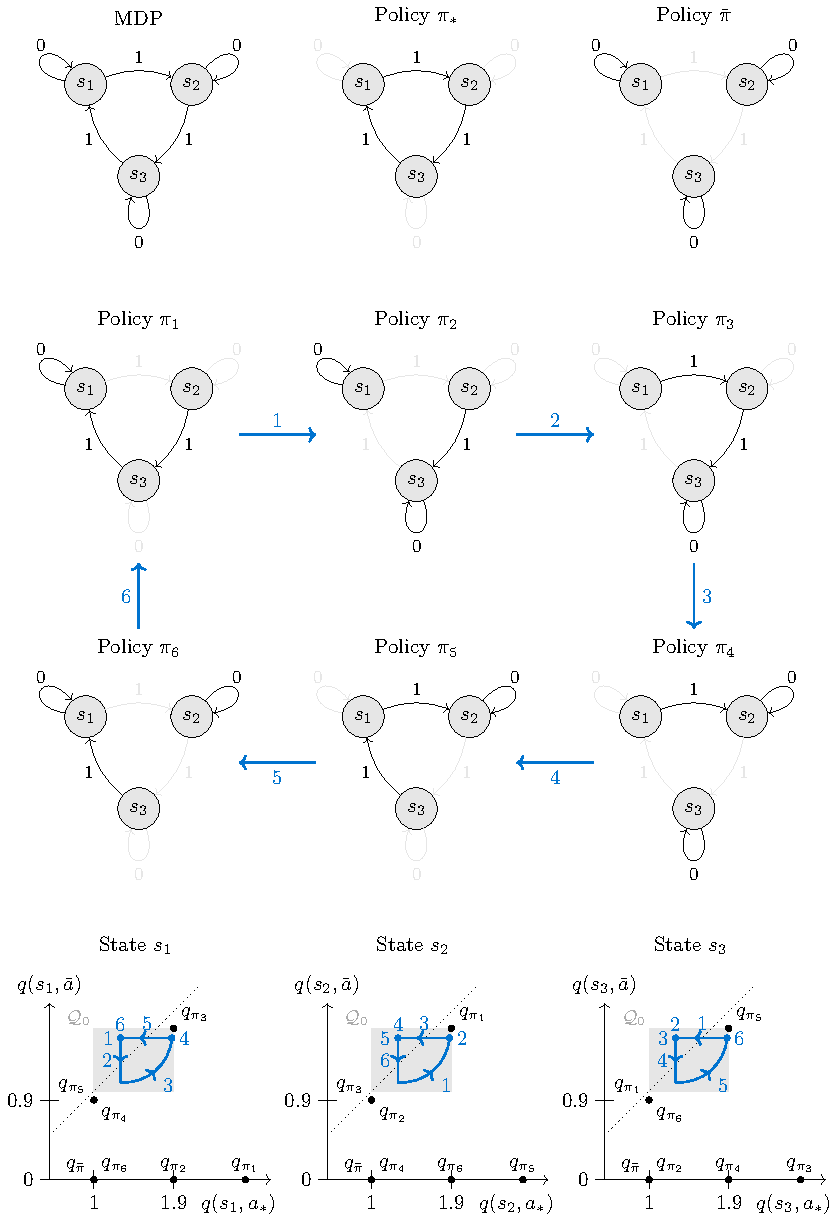
\includegraphics[width=0.95\textwidth]{figures/explain-loop-fig.pdf}
%     \pgfmathsetmacro{\shei}{0.9*1.73}
%     \pgfmathsetmacro{\swid}{0.9*2}
%     \pgfmathsetmacro{\lwid}{0.8}
    
%     \begin{subfigure}[b]{0.33\textwidth}
%         \centering
%         \begin{tikzpicture}[
%             scale=1, auto, node distance=2cm, 
%             every edge/.style={draw, <-, font=\small},
%             state/.style={circle, fill=mylightgrey, draw=black, text=black}
%         ]
%             \node at (\swid/2,\shei) [above, font=\normalsize, color=black, yshift=25pt] {MDP};
            
%             % Nodes
%             \node[state] (s1) at (0,\shei) {$s_1$};
%             \node[state] (s2) at (\swid,\shei) {$s_2$};
%             \node[state] (s3) at (\swid/2,0) {$s_3$};
%             % Edges
%             \path[->]
%                 (s1) edge[out=130, in=170, loop, looseness=8] node[pos=0.5, above] {$0$} (s1)
%                 (s2) edge[bend right=20] node[pos=0.5, above] {$1$} (s1)

%                 (s2) edge[out=10, in=50, loop, looseness=8] node[pos=0.5, above] {$0$} (s2)
%                 (s3) edge[bend right=20] node[pos=0.7, xshift=3, below] {$1$} (s2)
                
%                 (s3) edge[out=250, in=290, loop, looseness=8] node[pos=0.5, below] {$0$} (s3)
%                 (s1) edge[bend right=20] node[pos=0.3, xshift=-3, below] {$1$} (s3);
%         \end{tikzpicture}
%         % \caption{MDP}
%         \label{fig: off-policy MDP}
%     \end{subfigure}%
%     \hfill
%     \begin{subfigure}[b]{0.33\textwidth}
%         \centering
%         \begin{tikzpicture}[
%             scale=1, auto, node distance=2cm, 
%             every edge/.style={draw, <-, font=\small},
%             state/.style={circle, fill=mylightgrey, draw=black, text=black}
%         ]
%             \node at (\swid/2,\shei) [above, font=\normalsize, color=black, yshift=25pt] {Policy $\pi_*$};
        
%             % Nodes
%             \node[state] (s1) at (0,\shei) {$s_1$};
%             \node[state] (s2) at (\swid,\shei) {$s_2$};
%             \node[state] (s3) at (\swid/2,0) {$s_3$};
%             % Edges
%             \path[->]
%                 (s1) edge[out=130, in=170, loop, looseness=8, draw=mylightgrey] node[pos=0.5, above, text=mylightgrey] {$0$} (s1)
%                 (s2) edge[bend right=20] node[pos=0.5, above] {$1$} (s1)

%                 (s2) edge[out=10, in=50, loop, looseness=8, draw=mylightgrey] node[pos=0.5, above, text=mylightgrey] {$0$} (s2)
%                 (s3) edge[bend right=20] node[pos=0.7, xshift=3, below] {$1$} (s2)
                
%                 (s3) edge[out=250, in=290, loop, looseness=8, draw=mylightgrey] node[pos=0.5, below, text=mylightgrey] {$0$} (s3)
%                 (s1) edge[bend right=20] node[pos=0.3, xshift=-3, below] {$1$} (s3);
%         \end{tikzpicture}
%         % \caption{Policy $\best{\pol}$}
%     \end{subfigure}%
%     \hfill
%     \begin{subfigure}[b]{0.33\textwidth}
%         \centering
%         \begin{tikzpicture}[
%             scale=1, auto, node distance=2cm, 
%             every edge/.style={draw, <-, font=\small},
%             state/.style={circle, fill=mylightgrey, draw=black, text=black}
%         ]

%             \node at (\swid/2,\shei) [above, font=\normalsize, color=black, yshift=25pt] {Policy $\bar \pi$};
        
%             % Nodes
%             \node[state] (s1) at (0,\shei) {$s_1$};
%             \node[state] (s2) at (\swid,\shei) {$s_2$};
%             \node[state] (s3) at (\swid/2,0) {$s_3$};
%             % Edges
%             \path[->]
%                 (s1) edge[out=130, in=170, loop, looseness=8] node[pos=0.5, above] {$0$} (s1)
%                 (s2) edge[bend right=20, draw=mylightgrey] node[pos=0.5, above, text=mylightgrey] {$1$} (s1)

%                 (s2) edge[out=10, in=50, loop, looseness=8] node[pos=0.5, above] {$0$} (s2)
%                 (s3) edge[bend right=20, draw=mylightgrey] node[pos=0.7, xshift=3, below, text=mylightgrey] {$1$} (s2)
                
%                 (s3) edge[out=250, in=290, loop, looseness=8] node[pos=0.5, below] {$0$} (s3)
%                 (s1) edge[bend right=20, draw=mylightgrey] node[pos=0.3, xshift=-3, below, text=mylightgrey] {$1$} (s3);
%         \end{tikzpicture}
%         % \caption{Policy $\worst{\pol}$}
%     \end{subfigure}
   
%     \vfill
%     \vspace{0.8cm}

%     \begin{subfigure}[b]{0.33\textwidth}
%         \centering
%         \begin{tikzpicture}[
%             scale=1, auto, node distance=2cm, 
%             every edge/.style={draw, <-, font=\small},
%             state/.style={circle, fill=mylightgrey, draw=black, text=black}
%         ]
%             \node at (\swid/2,\shei) [above, font=\normalsize, color=black, yshift=25pt] {Policy $\pi_1$};

%             % Nodes
%             \node[state] (s1) at (0,\shei) {$s_1$};
%             \node[state] (s2) at (\swid,\shei) {$s_2$};
%             \node[state] (s3) at (\swid/2,0) {$s_3$};
%             % Edges
%             \path[->]
%                 (s1) edge[out=130, in=170, loop, looseness=8] node[pos=0.5, above] {$0$} (s1)
%                 (s2) edge[bend right=20, draw=mylightgrey] node[pos=0.5, above, text=mylightgrey] {$1$} (s1)

%                 (s2) edge[out=10, in=50, loop, looseness=8, draw=mylightgrey] node[pos=0.5, above, text=mylightgrey] {$0$} (s2)
%                 (s3) edge[bend right=20] node[pos=0.7, xshift=3, below] {$1$} (s2)
                
%                 (s3) edge[out=250, in=290, loop, looseness=8, draw=mylightgrey] node[pos=0.5, below, text=mylightgrey] {$0$} (s3)
%                 (s1) edge[bend right=20] node[pos=0.3, xshift=-3, below] {$1$} (s3);
% %            \draw[->,thick,red] (\swid+1,\shei/2) -- (\swid+2,\shei/2);    
%             % Cycle arrow: \pol_1 \to \pol_2.
%             \draw[overlay, ->, CambridgeCoreBlue, line width=\lwid pt]
%                 ({\swid+0.8},{\shei/2}) -- node[pos=0.5, above] {$1$} ({\swid+2.1},{\shei/2});
%             \draw[overlay, <-, CambridgeCoreBlue, line width=\lwid pt]
%                 ({\swid/2},{-1.4}) -- node[pos=0.5, left] {$6$} ({\swid/2},{-2.5});
%             % \draw[overlay, <-, CambridgeCoreBlue, line width=\lwid pt] 
%             %     (0,{-0.7}) 
%             %     to[out=225, in=135]
%             %     node[pos=0.5, left] {$6$} 
%             %     (0,{-2.7});
%         \end{tikzpicture}
%         % \caption{Policy $\pol_1$}
%     \end{subfigure}%
%     \hfill
%     \begin{subfigure}[b]{0.33\textwidth}
%         \centering
%         \begin{tikzpicture}[
%             scale=1, auto, node distance=2cm, 
%             every edge/.style={draw, <-, font=\small},
%             state/.style={circle, fill=mylightgrey, draw=black, text=black}
%         ]

%             \node at (\swid/2,\shei) [above, font=\normalsize, color=black, yshift=25pt] {Policy $\pi_2$};
        
%             % Nodes
%             \node[state] (s1) at (0,\shei) {$s_1$};
%             \node[state] (s2) at (\swid,\shei) {$s_2$};
%             \node[state] (s3) at (\swid/2,0) {$s_3$};
%             % Edges
%             \path[->]
%                 (s1) edge[out=130, in=170, loop, looseness=8] node[pos=0.5, above] {$0$} (s1)
%                 (s2) edge[bend right=20, draw=mylightgrey] node[pos=0.5, above, text=mylightgrey] {$1$} (s1)

%                 (s2) edge[out=10, in=50, loop, looseness=8, draw=mylightgrey] node[pos=0.5, above, text=mylightgrey] {$0$} (s2)
%                 (s3) edge[bend right=20] node[pos=0.7, xshift=3, below] {$1$} (s2)
                
%                 (s3) edge[out=250, in=290, loop, looseness=8] node[pos=0.5, below] {$0$} (s3)
%                 (s1) edge[bend right=20, draw=mylightgrey] node[pos=0.3, xshift=-3, below, text=mylightgrey] {$1$} (s3);
% %                            \draw[->,thick,red] (\swid+1,\shei/2) -- (\swid+2,\shei/2);    
%             % Cycle arrow: \pol_2 \to \pol_3.
%             % \draw[overlay, ->, CambridgeCoreBlue, line width=\lwid pt]
%             % ({\swid+0.8},{\shei/2}) -- node[pos=0.5, above] {$2$}  ({\swid+2.1},{\shei/2});
%         \end{tikzpicture}
%         % \caption{Policy $\pol_2$}
%     \end{subfigure}%
%     \hfill
%     \begin{subfigure}[b]{0.33\textwidth}
%         \centering
%         \begin{tikzpicture}[
%             scale=1, auto, node distance=2cm, 
%             every edge/.style={draw, <-, font=\small},
%             state/.style={circle, fill=mylightgrey, draw=black, text=black}
%         ]
%             \node at (\swid/2,\shei) [above, font=\normalsize, color=black, yshift=25pt] {Policy $\pi_3$};
        
%             % Nodes
%             \node[state] (s1) at (0,\shei) {$s_1$};
%             \node[state] (s2) at (\swid,\shei) {$s_2$};
%             \node[state] (s3) at (\swid/2,0) {$s_3$};
%             % Edges
%             \path[->]
%                 (s1) edge[out=130, in=170, loop, looseness=8, draw=mylightgrey] node[pos=0.5, above, text=mylightgrey] {$0$} (s1)
%                 (s2) edge[bend right=20] node[pos=0.5, above] {$1$} (s1)

%                 (s2) edge[out=10, in=50, loop, looseness=8, draw=mylightgrey] node[pos=0.5, above, text=mylightgrey] {$0$} (s2)
%                 (s3) edge[bend right=20] node[pos=0.7, xshift=3, below] {$1$} (s2)
                
%                 (s3) edge[out=250, in=290, loop, looseness=8] node[pos=0.5, below] {$0$} (s3)
%                 (s1) edge[bend right=20, draw=mylightgrey] node[pos=0.3, xshift=-3, below, text=mylightgrey] {$1$} (s3);
% %                            \draw[->,thick,red] (\swid+1,\shei/2) -- (\swid+1,\shei/2-4);
%             % Cycle arrow: \pol_3 \to \pol_4, routed outside the right edge
%             % so it does not cross the captions.
%             % \draw[overlay, ->, >=stealth, CambridgeCoreBlue, line width=1.7pt, shorten >=2pt]
%             %     ({\swid-0.1},{-0.10})
%             %         .. controls ({\swid+1.5},{-0.75}) and ({\swid+1.65},{-2.55}) ..
%             %     ({\swid-0.1},{-2.9});
%                 \draw[overlay, ->, CambridgeCoreBlue, line width=\lwid pt] 
%                 % ({\swid},{-0.7}) 
%                 % to[out=-45, in=45] 
%                 % node[pos=0.5, right] {$3$} 
%                 % ({\swid},{-2.7});
%                 ({\swid/2},{-1.4}) -- node[pos=0.5, right] {$3$} ({\swid/2},{-2.5});
                
%                 % ({\swid+0.45},{-0.10})
%                 %     .. controls ({\swid+1.65},{-0.75}) and ({\swid+1.65},{-2.55}) ..
%                 % ({\swid+0.95},{-3.25});

%                 \draw[overlay, <-, CambridgeCoreBlue, line width=\lwid pt]
%                 ({-0.8},{\shei/2}) -- node[pos=0.5, above] {$2$}  ({-2.1},{\shei/2});
%         \end{tikzpicture}
%         % \caption{Policy $\pol_3$}
%     \end{subfigure}
   
%     \vfill
%     \vspace{1.2cm}

%     \begin{subfigure}[b]{0.33\textwidth}
%         \centering
%         \begin{tikzpicture}[
%             scale=1, auto, node distance=2cm, 
%             every edge/.style={draw, <-, font=\small},
%             state/.style={circle, fill=mylightgrey, draw=black, text=black}
%         ]

%             \node at (\swid/2,\shei) [above, font=\normalsize, color=black, yshift=25pt] {Policy $\pi_6$};
        
%             % Nodes
%             \node[state] (s1) at (0,\shei) {$s_1$};
%             \node[state] (s2) at (\swid,\shei) {$s_2$};
%             \node[state] (s3) at (\swid/2,0) {$s_3$};
%             % Edges
%             \path[->]
%                 (s1) edge[out=130, in=170, loop, looseness=8] node[pos=0.5, above] {$0$} (s1)
%                 (s2) edge[bend right=20, draw=mylightgrey] node[pos=0.5, above, text=mylightgrey] {$1$} (s1)

%                 (s2) edge[out=10, in=50, loop, looseness=8] node[pos=0.5, above] {$0$} (s2)
%                 (s3) edge[bend right=20, draw=mylightgrey] node[pos=0.7, xshift=3, below, text=mylightgrey] {$1$} (s2)
                
%                 (s3) edge[out=250, in=290, loop, looseness=8, draw=mylightgrey] node[pos=0.5, below, text=mylightgrey] {$0$} (s3)
%                 (s1) edge[bend right=20] node[pos=0.3, xshift=-3, below] {$1$} (s3);
%             % Cycle arrow: \pol_6 \to \pol_1, routed outside the left edge
%             % so it does not cross the captions.
%             % \draw[overlay, ->, >=stealth, CambridgeCoreBlue, line width=1.7pt, shorten >=2pt]
%             %     ({-0.75},{\shei+0.10})
%             %         .. controls ({-1.65},{\shei+0.75}) and ({-1.65},{\shei+2.55}) ..
%             %     ({-0.95},{\shei+3.25});
%             % \draw[overlay, ->, CambridgeCoreBlue, line width=\lwid pt] 
%             %     (0,{\shei+0.10}) 
%             %     to[out=135, in=225]
%             %     node[pos=0.5, left] {$6$} 
%             %     (0,{\shei+3.25});
%             \draw[overlay, <-, CambridgeCoreBlue, line width=\lwid pt]
%                 ({\swid+0.8},{\shei/2}) -- node[pos=0.5, below] {$5$} ({\swid+2.1},{\shei/2});
%         \end{tikzpicture}
%         % \caption{Policy $\pol_6$}
%     \end{subfigure}
%    \hfill
%     \begin{subfigure}[b]{0.33\textwidth}
%         \centering
%         \begin{tikzpicture}[
%             scale=1, auto, node distance=2cm, 
%             every edge/.style={draw, <-, font=\small},
%             state/.style={circle, fill=mylightgrey, draw=black, text=black}
%         ]
%             \node at (\swid/2,\shei) [above, font=\normalsize, color=black, yshift=25pt] {Policy $\pi_5$};
        
%             % Nodes
%             \node[state] (s1) at (0,\shei) {$s_1$};
%             \node[state] (s2) at (\swid,\shei) {$s_2$};
%             \node[state] (s3) at (\swid/2,0) {$s_3$};
%             % Edges
%             \path[->]
%                 (s1) edge[out=130, in=170, loop, looseness=8, draw=mylightgrey] node[pos=0.5, above, text=mylightgrey] {$0$} (s1)
%                 (s2) edge[bend right=20] node[pos=0.5, above] {$1$} (s1)

%                 (s2) edge[out=10, in=50, loop, looseness=8] node[pos=0.5, above] {$0$} (s2)
%                 (s3) edge[bend right=20, draw=mylightgrey] node[pos=0.7, xshift=3, below, text=mylightgrey] {$1$} (s2)
                
%                 (s3) edge[out=250, in=290, loop, looseness=8, draw=mylightgrey] node[pos=0.5, below, text=mylightgrey] {$0$} (s3)
%                 (s1) edge[bend right=20] node[pos=0.3, xshift=-3, below] {$1$} (s3);
%             % Cycle arrow: \pol_5 \to \pol_6.
%             % \draw[overlay, ->, CambridgeCoreBlue, line width=\lwid pt]
%             %     ({-0.55},{\shei/2}) -- node[pos=0.5, below] {$5$} ({-2.25},{\shei/2});
%         \end{tikzpicture}
%         % \caption{Policy $\pol_5$}
%     \end{subfigure}%
%     \hfill
%  \begin{subfigure}[b]{0.33\textwidth}
%         \centering
%         \begin{tikzpicture}[
%             scale=1, auto, node distance=2cm, 
%             every edge/.style={draw, <-, font=\small},
%             state/.style={circle, fill=mylightgrey, draw=black, text=black}
%         ]
%             \node at (\swid/2,\shei) [above, font=\normalsize, color=black, yshift=25pt] {Policy $\pi_4$};
        
%             % Nodes
%             \node[state] (s1) at (0,\shei) {$s_1$};
%             \node[state] (s2) at (\swid,\shei) {$s_2$};
%             \node[state] (s3) at (\swid/2,0) {$s_3$};
%             % Edges
%             \path[->]
%                 (s1) edge[out=130, in=170, loop, looseness=8, draw=mylightgrey] node[pos=0.5, above, text=mylightgrey] {$0$} (s1)
%                 (s2) edge[bend right=20] node[pos=0.5, above] {$1$} (s1)

%                 (s2) edge[out=10, in=50, loop, looseness=8] node[pos=0.5, above] {$0$} (s2)
%                 (s3) edge[bend right=20, draw=mylightgrey] node[pos=0.7, xshift=3, below, text=mylightgrey] {$1$} (s2)
                
%                 (s3) edge[out=250, in=290, loop, looseness=8] node[pos=0.5, below] {$0$} (s3)
%                 (s1) edge[bend right=20, draw=mylightgrey] node[pos=0.3, xshift=-3, below, text=mylightgrey] {$1$} (s3);
%             % Cycle arrow: \pol_4 \to \pol_5.
%             \draw[overlay, ->, CambridgeCoreBlue, line width=\lwid pt]
%                 ({-0.8},{\shei/2}) -- node[pos=0.5, below] {$4$}  ({-2.1},{\shei/2});
%         \end{tikzpicture}
%         % \caption{Policy $\pol_4$}
%     \end{subfigure}%
    
%     \vspace{0.8cm}
   
%    \begin{subfigure}[b]{.32\textwidth}
%         \centering
%         \normalsize{State $s_1$}
        
%         {\begin{tikzpicture}[scale=1.5]
%             % Draw the grid and axes
%             % \draw[step=0.5cm,very thin,mylightgrey] (0,0) grid (3,3);
%             \draw[thin,->] (.5,0) -- (3,0) node[below left, xshift=6pt, yshift=-3pt] {$q(s_1,\best{a})$};
%             \draw[thin,->] (0.5,0) -- (0.5,2) node[above] {$q(s_1,\worst{a})$};
%             % \draw[thick,->] (0,0) -- (3.2,0) node[right] {\shortstack{$\best{a}$ \\ $\pol_1, \pol_5, \pol_6$}};
%             % \draw[thick,->] (0,0) -- (0,2.2) node[above] {\shortstack{$\worst{a}$ \\ $\pol_2, \pol_3, \pol_4$}};

%             \node at (1, 1.71) [above left, font=\small, color=mygrey, xshift=2pt, yshift=-2pt] {$\mathcal Q_0$};

%             % Draw the grey square from (1,1) to (2,2)
%             \filldraw[fill=mylightgrey, draw=none] (1,1) rectangle (1.9,1.71);
            
%             % Draw the line y = x
%             \draw[dotted, black] (0.5,0.5) -- (2.2,2.2);

%             % Add the points with associated text
%             \filldraw (2.71,0) circle (1pt) node[above] {$q_{\pol_1}$};
%             \filldraw (1.9,1.71) circle (1pt) node[above right] {$q_{\pol_3}$};
%             \filldraw (1.9,0) circle (1pt) node[above] {$q_{\pol_2}$};
%             \filldraw (1,0.9) circle (1pt) node[above left] {$q_{\pol_5}$};
%             \filldraw (1,0.9) circle (1pt) node[below right] {$q_{\pol_4}$};
%             \filldraw (1,0) circle (1pt) node[above right] {$q_{\pol_6}$};
%             \filldraw (1,0) circle (1pt) node[above left] {$q_{\worst{\pol}}$};
            
%             % Add labels to the axes
%             % \draw (0,0.1) -- (0,-0.1) node[left, font=\normalsize, xshift=-4.5pt, yshift=-6.5pt] {0};
%             %\draw (0,0.1) -- (0,-0.1) node[below, font=\normalsize] {0};
% %            \draw (-0.1,0) -- (0.1,0) node[font=\normalsize] {};
%             \foreach \x in {1,1.9}
%                 \draw (\x,0.1) -- (\x,-0.1) node[below, font=\normalsize] {\x};
%             \foreach \y in {0,0.9}
%                 \draw (.5+0.1,\y) -- (.5-0.1,\y) node[left, font=\normalsize] {\y};

%             % Add the red arrows
%             \draw[middle arrow=0.65, CambridgeCoreBlue, line width=\lwid pt] (1.9, 1.6) -- (1.3, 1.6) node[midway, above, sloped, font=\normalsize] {$5$};
%             \draw[middle arrow=0.55, CambridgeCoreBlue, line width=\lwid pt] (1.3, 1.6) -- (1.3, 1.1) node[midway, left, font=\normalsize] {$2$};
%             % \draw[middle arrow=0.5, CambridgeCoreBlue, thick] (1.3, 1.1) -- (1.9, 1.7) node[midway, below, sloped, font=\normalsize] {3};

%             \draw[middle arrow=0.5, CambridgeCoreBlue, line width=\lwid pt] 
%             (1.3,1.1) to[bend right=45] 
%             node[midway, below right, font=\normalsize] {$3$}
%             (1.88,1.6);

%             % \draw[thick, CambridgeCoreBlue] (1.45, 1.7) -- (1.45, 1.25);

%             \filldraw[fill=CambridgeCoreBlue, draw=CambridgeCoreBlue] (1.3,1.6) circle (1pt) node[left, text=CambridgeCoreBlue, font=\normalsize] {$1$};
%             \filldraw[fill=CambridgeCoreBlue, draw=CambridgeCoreBlue] (1.3,1.6) circle (0pt) node[above, text=CambridgeCoreBlue, font=\normalsize] {$6$};
%             \filldraw[fill=CambridgeCoreBlue, draw=CambridgeCoreBlue] (1.88,1.6) circle (1pt) node[right, text=CambridgeCoreBlue, font=\normalsize] {$4$};
            
%         \end{tikzpicture}}
%         % \caption{State $s_1$}
%         \end{subfigure}
%            \begin{subfigure}[b]{.32\textwidth}
%         \centering
%         \normalsize{State $s_2$}
        
%         {\begin{tikzpicture}[scale=1.5]
%             % Draw the grid and axes
%             % \draw[step=0.5cm,very thin,mylightgrey] (0,0) grid (3,3);
%             \draw[thin,->] (.5,0) -- (3,0) node[below left, xshift=6pt, yshift=-3pt] {$q(s_2,\best{a})$};
%             \draw[thin,->] (0.5,0) -- (0.5,2) node[above] {$q(s_2,\worst{a})$};
%             % \draw[thick,->] (0,0) -- (3.2,0) node[right] {\shortstack{$\best{a}$ \\ $\pol_1, \pol_5, \pol_6$}};
%             % \draw[thick,->] (0,0) -- (0,2.2) node[above] {\shortstack{$\worst{a}$ \\ $\pol_2, \pol_3, \pol_4$}};

%             % \node at (1.6, 2.2) [above, font=\normalsize, color=black] {State $s_1$};

%             \node at (1, 1.71) [above left, font=\small, color=mygrey, xshift=2pt, yshift=-2pt] {$\mathcal Q_0$};

%             % Draw the grey square from (1,1) to (2,2)
%             \filldraw[fill=mylightgrey, draw=none] (1,1) rectangle (1.9,1.71);
            
%             % Draw the line y = x
%             \draw[dotted, black] (0.5,0.5) -- (2.2,2.2);

%             % Add the points with associated text
%             \filldraw (2.71,0) circle (1pt) node[above] {$q_{\pol_5}$};
%             \filldraw (1.9,1.71) circle (1pt) node[above right] {$q_{\pol_1}$};
%             \filldraw (1.9,0) circle (1pt) node[above] {$q_{\pol_6}$};
%             \filldraw (1,0.9) circle (1pt) node[above left] {$q_{\pol_3}$};
%             \filldraw (1,0.9) circle (1pt) node[below right] {$q_{\pol_2}$};
%             \filldraw (1,0) circle (1pt) node[above right] {$q_{\pol_4}$};
%             \filldraw (1,0) circle (1pt) node[above left] {$q_{\worst{\pol}}$};
            
%             % Add labels to the axes
%             % \draw (0,0.1) -- (0,-0.1) node[left, font=\normalsize, xshift=-4.5pt, yshift=-6.5pt] {0};
%             %\draw (0,0.1) -- (0,-0.1) node[below, font=\normalsize] {0};
% %            \draw (-0.1,0) -- (0.1,0) node[font=\normalsize] {};
%             \foreach \x in {1,1.9}
%                 \draw (\x,0.1) -- (\x,-0.1) node[below, font=\normalsize] {\x};
%             \foreach \y in {0,0.9}
%                 \draw (.5+0.1,\y) -- (.5-0.1,\y) node[left, font=\normalsize] {\y};

%             % Add the red arrows
%             \draw[middle arrow=0.65, CambridgeCoreBlue, line width=\lwid pt] (1.9, 1.6) -- (1.3, 1.6) node[midway, above, sloped, font=\normalsize] {$3$};
%             \draw[middle arrow=0.55, CambridgeCoreBlue, line width=\lwid pt] (1.3, 1.6) -- (1.3, 1.1) node[midway, left, font=\normalsize] {$6$};
%             % \draw[middle arrow=0.5, CambridgeCoreBlue, thick] (1.3, 1.1) -- (1.9, 1.7) node[midway, below, sloped, font=\normalsize] {3};

%             \draw[middle arrow=0.5, CambridgeCoreBlue, line width=\lwid pt] 
%             (1.3,1.1) to[bend right=45] 
%             node[midway, below right, font=\normalsize] {$1$}
%             (1.88,1.6);

%             % \draw[thick, CambridgeCoreBlue] (1.45, 1.7) -- (1.45, 1.25);

%             \filldraw[fill=CambridgeCoreBlue, draw=CambridgeCoreBlue] (1.3,1.6) circle (1pt) node[left, text=CambridgeCoreBlue, font=\normalsize] {$5$};
%             \filldraw[fill=CambridgeCoreBlue, draw=CambridgeCoreBlue] (1.3,1.6) circle (0pt) node[above, text=CambridgeCoreBlue, font=\normalsize] {$4$};
%             \filldraw[fill=CambridgeCoreBlue, draw=CambridgeCoreBlue] (1.88,1.6) circle (1pt) node[right, text=CambridgeCoreBlue, font=\normalsize] {$2$};
            
%         \end{tikzpicture}}
%         % \caption{State $s_3$}
%         \end{subfigure}
%            \begin{subfigure}[b]{.32\textwidth}
%         \centering
%         \normalsize{State $s_3$}
        
%         {\begin{tikzpicture}[scale=1.5]
%             % Draw the grid and axes
%             % \draw[step=0.5cm,very thin,mylightgrey] (0,0) grid (3,3);
%             \draw[thin,->] (.5,0) -- (3,0) node[below left, xshift=6pt, yshift=-3pt] {$q(s_3,\best{a})$};
%             \draw[thin,->] (0.5,0) -- (0.5,2) node[above] {$q(s_3,\worst{a})$};
%             % \draw[thick,->] (0,0) -- (3.2,0) node[right] {\shortstack{$\best{a}$ \\ $\pol_1, \pol_5, \pol_6$}};
%             % \draw[thick,->] (0,0) -- (0,2.2) node[above] {\shortstack{$\worst{a}$ \\ $\pol_2, \pol_3, \pol_4$}};

%             % \node at (1.6, 2.2) [above, font=\normalsize, color=black] {State $s_1$};

%             \node at (1, 1.71) [above left, font=\small, color=mygrey, xshift=2pt, yshift=-2pt] {$\mathcal Q_0$};

%             % Draw the grey square from (1,1) to (2,2)
%             \filldraw[fill=mylightgrey, draw=none] (1,1) rectangle (1.9,1.71);
            
%             % Draw the line y = x
%             \draw[dotted, black] (0.5,0.5) -- (2.2,2.2);

%             % Add the points with associated text
%             \filldraw (2.71,0) circle (1pt) node[above] {$q_{\pol_3}$};
%             \filldraw (1.9,1.71) circle (1pt) node[above right] {$q_{\pol_5}$};
%             \filldraw (1.9,0) circle (1pt) node[above] {$q_{\pol_4}$};
%             \filldraw (1,0.9) circle (1pt) node[above left] {$q_{\pol_1}$};
%             \filldraw (1,0.9) circle (1pt) node[below right] {$q_{\pol_6}$};
%             \filldraw (1,0) circle (1pt) node[above right] {$q_{\pol_2}$};
%             \filldraw (1,0) circle (1pt) node[above left] {$q_{\worst{\pol}}$};
            
%             % Add labels to the axes
%             % \draw (0,0.1) -- (0,-0.1) node[left, font=\normalsize, xshift=-4.5pt, yshift=-6.5pt] {0};
%             %\draw (0,0.1) -- (0,-0.1) node[below, font=\normalsize] {0};
% %            \draw (-0.1,0) -- (0.1,0) node[font=\normalsize] {};
%             \foreach \x in {1,1.9}
%                 \draw (\x,0.1) -- (\x,-0.1) node[below, font=\normalsize] {\x};
%             \foreach \y in {0,0.9}
%                 \draw (.5+0.1,\y) -- (.5-0.1,\y) node[left, font=\normalsize] {\y};

%             % Add the red arrows
%             \draw[middle arrow=0.65, CambridgeCoreBlue, line width=\lwid pt] (1.9, 1.6) -- (1.3, 1.6) node[midway, above, sloped, font=\normalsize] {$1$};
%             \draw[middle arrow=0.55, CambridgeCoreBlue, line width=\lwid pt] (1.3, 1.6) -- (1.3, 1.1) node[midway, left, font=\normalsize] {$4$};
%             % \draw[middle arrow=0.5, CambridgeCoreBlue, thick] (1.3, 1.1) -- (1.9, 1.7) node[midway, below, sloped, font=\normalsize] {3};

%             \draw[middle arrow=0.5, CambridgeCoreBlue, line width=\lwid pt] 
%             (1.3,1.1) to[bend right=45] 
%             node[midway, below right, font=\normalsize] {$5$}
%             (1.88,1.6);

%             % \draw[thick, CambridgeCoreBlue] (1.45, 1.7) -- (1.45, 1.25);

%             \filldraw[fill=CambridgeCoreBlue, draw=CambridgeCoreBlue] (1.3,1.6) circle (1pt) node[left, text=CambridgeCoreBlue, font=\normalsize] {$3$};
%             \filldraw[fill=CambridgeCoreBlue, draw=CambridgeCoreBlue] (1.3,1.6) circle (0pt) node[above, text=CambridgeCoreBlue, font=\normalsize] {$2$};
%             \filldraw[fill=CambridgeCoreBlue, draw=CambridgeCoreBlue] (1.88,1.6) circle (1pt) node[right, text=CambridgeCoreBlue, font=\normalsize] {$6$};
            
%         \end{tikzpicture}}
%         % \caption{State $s_1$}
%         \end{subfigure}
    \caption{The sampling strategy described on page \pageref{pg: sampling strat 3 states} forces IV MC-O-PI to cycle indefinitely between six suboptimal policies
    % $\pol_1$, $\pol_2$, $\pol_3$, $\pol_4$, $\pol_5$ and $\pol_6$ 
    for every initial condition in $\qset_0$.
    This figure depicts the expected cycle in the policies $\{\pi_k\}_{k\ge 0}$ (middle) and in the estimates $\{q_k\}_{k\ge 0}$ (bottom).
    The "move" action correspond to $a_*$, and "stay" to $\bar a$.
    The dotted lines are the boundaries between regions, namely where $q(s,a_*) = q(s,\bar a)$.}
    % Spiral obtained for every initial condition in $\qset_0$ with the sampling strategy described on page \pageref{enum: sampling greedy initial visit}.
    % MC-O-PI cycles indefinitely between the policies $\pol_1$ through $\pol_6$ despite the update distributions with a greedy bias.}
    \label{fig: explain loop on-policy bias MDP}
    \end{figure}%



% \includepdf[pages=-]{figures/big-picture.pdf}


% describe bias / loop
The following sampling strategy forces IV MCES to cycle indefinitely between the suboptimal policies $\pol_1$, $\pol_2$, $\pol_3$, $\pol_4$, $\pol_5$ and $\pol_6$ for every initial condition in the region $\qset_0$, which 
is the intersection between the regions of these six policies and the shaded region in \autoref{fig: explain loop on-policy bias MDP}:
% consists of points which are in both the shaded region in \autoref{fig: explain loop on-policy bias MDP} and the greedy region of one of these policies:
\begin{enumerate}
    \item  \label{pg: sampling strat 3 states}
    When $q_k \in \region(\pol_1)$, start each episode in $(s_2, \best{a})$ or $(s_3, \best{a})$ with a probability of 0.4, or in $(s_2, \worst{a})$ with a probability of 0.2.
    % Given the initial-visit updates, this yields a greedy bias in states $s_2$ and $s_3$, and no updates in $s_1$.
    \mcopi{} is then expected to cross the boundary in state $s_3$ and transition to policy $\pol_2$.

    \item
    When $q_k \in \region(\pol_2)$, start each episode in $(s_1, \worst{a})$. 
    % The bias is greedy in $s_1$. There are no updates in $s_2$ and $s_3$.
    MCES will cross the boundary in $s_1$ and transition to $\pol_3$.

    \item
    When $q_k \in \region(\pol_3)$, start each episode in $(s_1, \best{a})$ or $(s_2, \best{a})$ with a probability of 0.4, or in $(s_1, \worst{a})$ with a probability of 0.2.
    % The bias is greedy in $s_1$ and $s_2$. There are no updates in $s_3$.
    \mcopi{} is then expected to cross the boundary in $s_2$ and transition to $\pol_4$.

    \item
    When $q_\kpz \in \region(\pol_4)$, start each episode in $(s_3, \worst{a})$. 
    % The bias is greedy in $s_3$. There are no updates in $s_1$ and $s_2$.
    MCES will cross the boundary in $s_3$ and transition to $\pol_5$.

    \item
    When $q_\kpz \in \region(\pol_5)$, start each episode in $(s_1, \best{a})$ or $(s_3, \best{a})$ with a probability of 0.4, or in $(s_3, \worst{a})$ with a probability of 0.2.
    % The bias is greedy in $s_1$ and $s_3$. There are no updates in $s_2$.
    \mcopi{} is then expected to cross the boundary in $s_1$ and transition to $\pol_6$.

    \item
    When $q_\kpz \in \region(\pol_6)$, start each episode in $(s_2, \worst{a})$. 
    % The bias is greedy in $s_2$. There are no updates in $s_1$ and $s_3$.
    \mcopi{} will cross the boundary in $s_2$ and transition to $\pol_1$.
\end{enumerate}
\label{enum: sampling greedy initial visit}

The cycle is robust to noise caused by sampling the initial state-action pairs in steps 1, 3 and 5.
For example, if $(s_2, \worst{a})$ is updated several times in a row during step 1, the solution might switch to policy $\pol_6$ instead of $\pol_2$.
Nevertheless, the update distribution under $\pol_6$ directly corrects this by updating $(s_2, \worst{a})$ and driving the solution back to $\pol_1$.
Thus, the sampling strategy guarantees that, for every initial condition in $\mathcal Q_0$, the greedy policy $\pi_k$ contains at least one suboptimal action but never all three.
As a result, 
solutions cycle indefinitely with potential pairwise repeats between $\pi_1$ and $\pi_6$, $\pi_3$ and $\pi_2$, or $\pi_4$ and $\pi_5$ but without ever visiting the policies $\best{\pol}$ or $\worst{\pol}$.
This behaviour does not rely on the exact probabilities above.
It persists when increasing the sampling bias towards greedy actions,
% $\best{a}$ during the diagonal movement upwards, 
for instance when replacing the 2-to-1 sampling ratio of $(s_2, \best{a})$ to $(s_2, \worst{a})$ during step 1 with an epsilon-greedy strategy for small epsilon.

We incorporate exploring starts 
% so that the algorithm samples the wrong state-action pair at the wrong time infinitely often.
% Specifically, we
by initialising each episode using the sampling strategy above with a probability of 0.9 
or by uniformly sampling a state-action pair with a probability of 0.1.
Since the wrong state-action pairs are now sampled at the wrong time infinitely often,
solutions can visit the policies $\best{\pol}$ or $\worst{\pol}$.
When they do, we sample the initial state-action pair uniformly.
Additionally, we introduce stochastic transitions by terminating each episode with a probability of 0.1 after each action.
% Policy evaluation is then stochastic.
The value $q_{\pol_k}(s,a)$ is then always over- or underestimated, which yields steps that potentially drive solutions out of $\qset_0$.


\begin{figure}[htbp]
    \pgfmathsetmacro{\xmin}{0.5}
    \pgfmathsetmacro{\xmax}{8.5}
    \pgfmathsetmacro{\ymin}{.5}
    \pgfmathsetmacro{\ymax}{6.5}
       \begin{subfigure}[b]{0.48\textwidth}
        \centering
        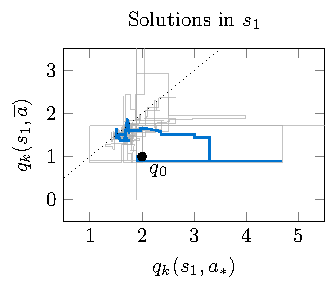
\includegraphics{figures/iv-simulation.pdf}
        % \begin{tikzpicture}[scale=1]
        %     \begin{axis}[
        %         xlabel={$q_k(s_1, \best{a})$},
        %         ylabel={$q_k(s_1, \worst{a})$},
        %         xmin=0.5, xmax=5.5,
        %         ymin=-0.5, ymax=3.5,
        %         xtick={1,2,...,5},
        %         ytick={0,1,2,...,3},
        %         title={Solutions in $s_1$},
        %         grid=none,
        %         % tick label style={font=\small},
        %         % label style={font=\small},
        %         width=0.9\linewidth,
        %         height=4.5cm,
        %     ]
        %         \pgfplotstableread[col sep=tab]{figures/33/3s_phase_st_s1.txt}\datatable
            
        %         \foreach \n in {1,...,9} {
        %             \pgfmathsetmacro\yindex{10+\n}
        %             \addplot [mygrey, opacity=0.7] table [x index=\n, y index=\yindex] {\datatable};
        %         }
        %         \addplot [CambridgeCoreBlue, line width=0.8pt] table [x index=0, y index=10] {\datatable};

        %         \addplot[color=black, mark=*, mark size=2pt] coordinates {(2, 1)};
        %         \node[text=black, below right] at (axis cs:2, 1) {$q_0$};
                
        %         \addplot[color=black, dotted, domain=\xmin:\xmax] {x};
    
        %     \end{axis}
        % \end{tikzpicture}
        % \caption{State $s_1$}
 \end{subfigure}%
 \hspace{0.5cm}
 \begin{subfigure}[b]{.48\textwidth}
        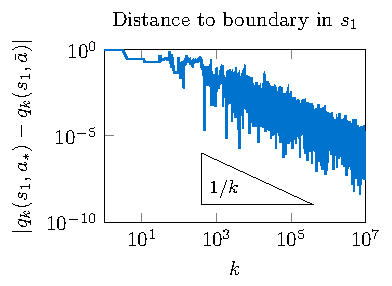
\includegraphics{figures/iv-contraction.pdf}
    %  \begin{tikzpicture}[scale=1]
    %     \begin{axis}[
    %         xmode=log,
    %         ymode=log,
    %         xlabel={$k$},
    %         ylabel={$\left|q_k(s_1,a_*)-q_k(s_1, \bar a)\right|$},
    %         grid=none,
    %         title={Distance to boundary in $s_1$},
    %         xmin=1, xmax=1e7,
    %         ymin=1e-10, ymax=1,
    %         width=0.9\linewidth,
    %         height=4.5cm,
    %     ]
    %     \addplot[
    %         CambridgeCoreBlue, line width=0.8pt
    %     ] table[
    %         x index=0,
    %         y index=1
    %     ] {figures/33/q_difference_loglog.txt};

    %     \draw[black] (axis cs:0.4*1e3,1e-9) -- (axis cs:0.4*1e6, 1e-9) -- (axis cs:0.4*1e3,1e-6) -- cycle;
    %     \node[above right, font=\small] at (axis cs:0.4*1e3, 1e-9) {$1/k$};
    %     \end{axis}
    % \end{tikzpicture}
 \end{subfigure}%
    \caption{Initial-visit MCES with sample-average updates can converge to a suboptimal solution where $q(s, a_*) = q(s, \bar a)$ for all states
    even when the greedy action is sampled at least as frequently as any other action in each state.
    % even when the sampling strategy satisfies exploring starts and the discounted MDP has stochastic transitions.
    The blue line depicts a representative solution.}
    % highlights one of ten simulations.
    % We obtain similar behaviours in states $s_2$ and $s_3$.}
    \label{fig: 3s IV ES ST}
    \vspace{-0.2cm}
\end{figure}


Despite the variability of initial state-action pairs and the noisy action-value estimates, IV MCES still converges to a suboptimal solution when using SA learning rates.
% $\eta_k(s,a) = 1/n_k(s,a)$.
For instance,
$99.6\%$ of solutions converge to a point where $q(s, a_*) = q(s, \bar a) \approx 1.615$ for all states
when starting in
$q_0(s_1,a_*) = q_0(s_2,a_*) = q_0(s_3,\bar a) = 2$
and
$q_0(s_1,\bar a) = q_0(s_2, \bar a) = q_0(s_3,a_*) = 1$
with $n_1(s,a)=1$ for all state-action pairs (\autoref{fig: 3s IV ES ST}).
The remaining $0.4\%$ escape to $q_{\pi_*}$.


% \autoref{fig: 3s IV ES ST} presents ten solutions,
% % of initial-visit \mcopi{} on the MDP with stochastic transitions and $\discount = 0.9$.
% all starting in
% $q_0(s_1,a_*) = q_0(s_1,a_*) = q_0(s_1,\bar a) = 2$
% and
% $q_0(s_1,\bar a) = q_0(s_1, \bar a) = q_0(s_1,a_*) = 1$.
% All ten solutions converge to a point where $q(s, a_*) = q(s, \bar a) \approx 1.615$ for each states. 
% {\color{red} please add following!}
% From an initial count of $n_1(s,a)=1$ for all state/action pairs approximately $99.6\%$ of solutions converge to the boundary near this point, with the remaining $0.4\%$ escaping to $q_{\pi_*}$.

% The graph on the right shows 

    % &q_0(s_1, \best{a}) = 2
    % \\
    % &q_0(s_1, \worst{a}) = 1 
    % \\
    % &q_0(s_2, \best{a}) = 2
    % \\
    % &q_0(s_2, \worst{a}) = 1 
    % \\
    % &q_0(s_3, \best{a}) = 1
    % \\
    % &q_0(s_3, \worst{a}) = 2
% We see that solutions regularly leave the region $\qset_0$ but still converge to the boundary around 1.61.
% We conclude that the conjecture of \citet[p.~99]{Sutton2018ReinforcementIntroduction} does not hold when replacing first-visit updates with initial-visit updates.


The reason solutions converge to the boundary despite frequently visiting the optimal policy $\pi_*$ is as follows.
Consider a solution in the region $Q(\pi_*)$ near the boundary point $1.615$.
So $q_k(s, a_*) > q_k(s, \bar a)$ 
% and $q_{\pi_*}(s, a_*) > q_{\pi_*}(s, \bar a)$ 
for every state,
and $q_k(s,a) < \qopt(s,a)$ for every state-action pair.
There are two possible updates.
Updating $(s, a_*)$ moves $q_k$ deeper into $Q(\pi_*)$ on average as $q_k(s, a_*)$ increases compared to $q_k(s, \bar a)$.
In contrast, updating $(s, \bar a)$ guides the solution towards the boundary of $Q(\pi_*)$ as $q_k(s, \bar a)$ catches up to $q_k(s, a_*)$. If the learning rate is large enough, 
$\bar a$ may even become greedy in $s$.
% the greedy action in $s$ may even change.
Thus, solutions consistently leave the optimal region only if 
updates to $(s, \bar a)$ receive larger learning rates or are more frequent on average than updates to $(s, a_*)$.
% vertical steps upwards are larger or more frequent on average than horizontal steps to the right.
% despite the uniform sampling strategy under policy $\best{\pol}$.
% {\color{red} Prefer something like: Precisely this behaviour is induced by ... - without the paragraph break, as it's continuing the argument is it not}
Precisely this behaviour is induced by the sampling strategy, the initial-visit updates and the sample-average learning rates.
Specifically, the sampling strategy 
% described 
% on page \pageref{pg: sampling strat 3 states}
% in \autoref{sec: 3 state sampling strat} 
combined with initial-visit updates implies that, for every state, $a_*$ is updated more frequently than $\bar a$ when solutions cycle between the policies $\pol_1$, $\pol_2$, $\pol_3$, $\pol_4$, $\pol_5$ and $\pol_6$.
Therefore, $1/n_k(s, \best{a})$ decreases faster than $1/n_k(s, \worst{a})$ for each state.
As a result, when noise pushes solutions into the optimal region $Q(\pi_*)$, all actions are updated equally frequently but updates to $(s, \worst{a})$ are larger than updates to $(s, \best{a})$,
% due to the difference in learning rates, 
which drives solutions out of $Q(\pi_*)$.
In other words, the sampling strategy, the initial-visit updates and the learning rates effectively bias updates towards suboptimal actions when $\pol_k = \best{\pol}$ even though greedy actions are updated more frequently. 
As discussed above, this 
% {\color{red} effective (at least add this, but I'd remove the phrase entirely, ie "this allows ...") } non-greedy bias 
allows solutions to consistently jump in and out of the optimal region, creating a stable suboptimal boundary region when the learning rates decrease.
% 
% {\color{red} delete this, it confuses the argument: Experiments show that this suboptimal asymptotic behaviour disappears when using scalar learning rates.
% Such learning rates assign the same step size to all state-action pairs. Thus they cannot introduce a non-greedy bias when sampling distributions favour greedy actions.}
% As a result, during some visit to $Q(\pi_*)$, solutions remain

Overall,
this example shows that IV/SA MCES may converge to suboptimal solutions even when, in each state, the greedy action is updated at least as frequently as any other action.
The asymptotic behaviour is determined by the interplay
between learning rates and within-state update frequencies, rather than either factor alone.
This suggests a remedy: scale learning rates to offset non-uniform update
frequencies in each state and recover convergence to optimality.


%%%%%%%%%%%%%%%%%%%%%%%%%%%%%%%%%%%%%%%%%%%%%%%%%%%%%%%%%%%%%%%
%%%%%%%%%%%%%%%%%%%%%%%%%%%%%%%%%%%%%%%%%%%%%%%%%%%%%%%%%%%%%%%
\section{Fix for initial-visit MCES}

Starting from an initial $q_0$,
IV MCES repeats the following steps for $k=0,1,\ldots,\infty$:
\begin{enumerate}
    \item Select a deterministic policy $\pi_k(s) \in \arg\max_a q_k(s,a)$ for all $s$.

    \item Sample an initial state-action pair $(s_k, a_k) \sim \sigma_k$.

    \item Update the estimate $q_k$ as
    \begin{align}
    \label{eq: update iv mcopi}
    q_{k+1}(s,a)
    =
    \begin{cases}
    q_k(s,a) + \eta_k(s,a) \left(\tilde q_k(s,a) - q_k(s,a) \right), & (s,a)=(s_k,a_k) \\
    % q_k(s,a) + \alpha_k \left(q_{\pi_k}(s,a)+v_k(s,a)-q_k(s,a) \right), & (s,a)=(s_k,a_k) \\ 
    q_k(s,a) & \text{otherwise .}
    \end{cases}
    \end{align}
    where $\tilde q_k$ is the episode return defined in \eqref{eq: episode return}.
\end{enumerate}

Section~\ref{sec: counterexample iv mces}, together with Appendix~\ref{app: non greedy} and Example~5.12 in \cite{Bertsekas1996Neuro-DynamicProgramming}, shows that IV MCES may converge to suboptimal solutions when the sampling distributions are biased towards either greedy or non-greedy actions.
This section presents a way to compensate for such non-uniform sampling by appropriately normalizing the learning rates, and thereby restoring convergence to optimality.
The approach relies on the chain rule decomposition of the sampling distribution:
\begin{align}
\label{eq: chain rule}
\sigma_k(s,a) = f_k(s) \, g_k(a | s) .
% \qquad 
% \forall \, k \ge 0, \
% \forall \, s \in \sset, \
% \forall \, a \in \aset(s) .
\end{align}


To formalise this correction, 
% Next, define the stochastic perturbation $v_k := g_k - q_{\pi_k}$.
% Under initial- or first-visit updates, $g_k$ is an unbiased estimate of $q_{\pi_k}$ with uniformly bounded variance
% \citep[Theorems 6 \& 8]{Singh1996ReinforcementTraces}.
% Thus there exists a constant $c_v \in [0,\infty)$ such that
% \begin{align}
% \label{eq: properties episode noise}
% \mathbb E\!\left[v_k(s,a) \mid \mathcal F_k \right] = 0 ,
% \qquad
% \mathbb E\!\left[v_k^2(s,a) \mid \mathcal F_k \right] \le c_v ,
% \qquad
% \forall \, k \ge 0, \
% \forall \, s \in \sset, \
% \forall \, a \in \aset(s) ,
% \end{align}
let $\mathcal F_k$ denote the information available after computing $q_k$,
but before selecting policy $\pi_k$, sampling the initial pair $(s_k, a_k)$, and generating the episode $\mathcal E_k$.
% We use the following assumptions.

% The standard GLIE (greedy in the limit with infinite exploration) conditions require that every state–action pair is visited infinitely often and that the policy $\pi_k$ becomes greedy with respect to $q_k$ as $k \to \infty$. The first condition guarantees sufficient exploration, while the second ensures that the optimal solution $(q_{\pi_*}, \pi_*)$ is a fixed point of the algorithm.
% Since our focus is on asymptotic behaviour, we may, without loss of generality, restrict attention to policies $\pi_k$ that are greedy with respect to $q_k$ at each iteration, as GLIE implies that any admissible exploration strategy becomes asymptotically equivalent to this greedy regime.

% \textcolor{red}{need to introduce $\polset$ somewhere}

% \begin{assumption}
% \label{asp: standing}
% \phantom{Assume}
% \begin{enumerate}[label=(\arabic*)]
%     \item \textbf{Discounted or episodic MDP.}
%     Either the discount factor satisfies $\gamma \in [0, 1)$ or each episode of the MDP almost surely reaches a terminal state.

%     \item \textbf{Uniform tie-breaking of greedy policies.}
%     There exists a constant \(\beta>0\) such that,
%     if several policies are greedy with respect to $q_k$,
%     \begin{equation}
%     \label{eq:greedy-pol-tie-breaking}
%     \mathbb P(\pi_k(a | s) = 1 \mid \mathcal F_k)\ge \beta,
%         \qquad 
%         \forall \, k \ge 0, \
%         \forall \, s \in \sset, \
%         \forall \, a \in \arg\max_{\mathcal A(s)} q_k(s,\cdot) .
%     \end{equation}

%     \item \textbf{Strict exploring starts.}
%     The sampling distributions $\{\sigma_k\}_{k \ge 0}$ satisfy
%     \begin{align}
%     \label{eq: strict exploring starts}
%         \sigma_k(s,a) \ge \sigma_{\min}
%         \qquad 
%         \forall \, k \ge 0, \
%         \forall \, s \in \sset, \
%         \forall \, a \in \aset(s) ,
%     \end{align}
%     for some constant $\sigma_{\min} \in (0,\infty)$.


%     \item \textbf{Scalar, Robbins--Monro and comparable learning rates.} 
%     The sequence $\{\alpha_k\}_{k \ge 0}$ forms a scalar non-increasing sequence: $\alpha_{k+1} \leq \alpha_k$ for every $k \ge 0$.
%     It satisfies
%     % The learning rates $(\eta_k)$ satisfy
%     \begin{align}
%     \label{eq: robbins monro conditions}
%         \sum_{k =0}^\infty \alpha_k = \infty , 
%         \qquad
%         \sum_{k =0}^\infty \alpha_k^2 < \infty ,
%     \end{align}
%     and there exist a time $K_\alpha < \infty$ and a constant $\rho_\alpha \in(0,1]$ such that
%     \begin{align}
%     \label{eq: comparability of learning rates}
%     \alpha_{k+i} \ge \rho_\alpha \alpha_k ,
%     \qquad
%     \forall \, k \ge K_\alpha, \
%     \forall \, i \in \{0, \dots, \left\lfloor 1 / \alpha_k \right\rfloor\} .
%     \end{align}
%     Given that condition \eqref{eq: robbins monro conditions} requires that $\alpha_k \to 0$ and we study the asymptotic behaviour of MCES, we assume, without loss of generality, that $\alpha_k \in (0, 1]$.
%     % \item \textbf{Initial-visit updates.} Only the initial state of each episode is updated.
%     % So the episode noise is unbiased and has bounded variance:
%     % \[
%     % \mathbb E\!\left[v_k(s,a) \mid \mathcal F_k \right] = 0 ,
%     % \qquad
%     % \mathbb E\!\left[v_k^2(s,a) \mid \mathcal F_k \right] \le c_v ,
%     % \qquad
%     % \forall \, k \ge 0, \
%     % \forall \, s \in \sset, \
%     % \forall \, a \in \aset(s).
%     % \]
%     % for some constant $c_v \in [0,\infty)$.
% \end{enumerate}
% \end{assumption}

% given that the episode returns are unbiased estimates of $q_{\pi_k}$ and have uniformly bounded variance \cite{Singh1996ReinforcementTraces}, there exists a constant $c_v \in [0,\infty)$ such that 
% $\mathbb E\!\left[v_k(s,a) \mid \mathcal F_k \right] = 0$
% and
% $\mathbb E\!\left[v_k^2(s,a) \mid \mathcal F_k \right] \le c_v$
% for every time $k \ge 0$, every state $s \in \mathcal S$ and every action $a \in \mathcal A(s)$.
% The sequence $\{v_k\}_{k \ge 0}$ is thus a martingale difference sequence adapted to the filtration $\{\mathcal F_{k}\}_{k \ge 0}$.


\begin{theorem}
\label{thm: iv mcopi with 1/g scaling}
Assume
\begin{enumerate}[label=(\arabic*)]
    \item \textbf{Discounted or episodic MDP.}
    Either the discount factor satisfies $\gamma \in [0, 1)$ or each episode of the MDP almost surely reaches a terminal state.

    \item \textbf{Uniform tie-breaking of greedy policies.}
    There exists a constant \(\beta>0\) such that,
    if several policies are greedy with respect to $q_k$,
    \begin{equation}
    \label{eq:greedy-pol-tie-breaking}
    \mathbb P(\pi_k(a | s) = 1 \mid \mathcal F_k)\ge \beta,
        \qquad 
        \forall \, k \ge 0, \
        \forall \, s \in \sset, \
        \forall \, a \in \arg\max_{\mathcal A(s)} q_k(s,\cdot) .
    \end{equation}

    \item \textbf{Strict exploring starts.}
    The sampling distributions $\{\sigma_k\}_{k \ge 0}$ satisfy
    \begin{align}
    \label{eq: strict exploring starts}
        \sigma_k(s,a) \ge \sigma_{\min}
        \qquad 
        \forall \, k \ge 0, \
        \forall \, s \in \sset, \
        \forall \, a \in \aset(s) ,
    \end{align}
    for some constant $\sigma_{\min} \in (0,\infty)$.


    \item \textbf{Scalar, Robbins--Monro and comparable learning rates.} 
    The sequence $\{\alpha_k\}_{k \ge 0}$ forms a scalar non-increasing sequence: $\alpha_{k+1} \leq \alpha_k$ for every $k \ge 0$.
    It satisfies
    % The learning rates $(\eta_k)$ satisfy
    \begin{align}
    \label{eq: robbins monro conditions}
        \sum_{k =0}^\infty \alpha_k = \infty , 
        \qquad
        \sum_{k =0}^\infty \alpha_k^2 < \infty ,
    \end{align}
    and there exist a time $K_\alpha < \infty$ and a constant $\rho_\alpha \in(0,1]$ such that
    \begin{align}
    \label{eq: comparability of learning rates}
    \alpha_{k+i} \ge \rho_\alpha \alpha_k ,
    \qquad
    \forall \, k \ge K_\alpha, \
    \forall \, i \in \{0, \dots, \left\lfloor 1 / \alpha_k \right\rfloor\} .
    \end{align}
    Given that condition \eqref{eq: robbins monro conditions} requires that $\alpha_k \to 0$ and we study the asymptotic behaviour of MCES, we assume, without loss of generality, that $\alpha_k \in (0, 1]$.
    % \item \textbf{Initial-visit updates.} Only the initial state of each episode is updated.
    % So the episode noise is unbiased and has bounded variance:
    % \[
    % \mathbb E\!\left[v_k(s,a) \mid \mathcal F_k \right] = 0 ,
    % \qquad
    % \mathbb E\!\left[v_k^2(s,a) \mid \mathcal F_k \right] \le c_v ,
    % \qquad
    % \forall \, k \ge 0, \
    % \forall \, s \in \sset, \
    % \forall \, a \in \aset(s).
    % \]
    % for some constant $c_v \in [0,\infty)$.
\end{enumerate}
% Take a sequence $\{\alpha_k\}_{k \ge 0}$ satisfying \autoref{asp: standing}.(4) and set the learning rate in \eqref{eq: update iv mcopi} as
Then IV MCES converges almost surely to $q_{\pi_*}$ when using learning rates
% learning rates
\begin{align}
\label{eq: normalised learning rates}
\eta_k(s,a) := \dfrac{\alpha_k}{g_k(a|s)} .
% \eta_k(s,a) := \dfrac{\alpha_k}{g_k(a|s) |\mathcal A(s)|} .
% \qquad 
% \forall \, k \ge 0 .
\end{align}
\end{theorem}


The scaling in \eqref{eq: normalised learning rates} is a local analogue of SA learning rates.
While $1/n_k(s,a)$ gives a greater weight to actions that have been sampled less often in the past,
the factor $1/g_k(a|s)$ gives a greater weight to actions which are less likely to be sampled at the current step.
The correction is thus local in time: it compensates for the current sampling bias rather than the historical sampling frequency.

The key idea in proving \autoref{thm: iv mcopi with 1/g scaling} is to analyse the sequence of policies $\{\pi_k\}_{k\ge 0}$ rather than the evolution of the estimates $\{q_k\}_{k\ge 0}$.
We find that the normalization in \eqref{eq: normalised learning rates}
causes the associated mean-field dynamics to generate monotonically improving policies
because it equalises the rate of change across actions on a state-by-state basis at every step.
This structure allows us to establish convergence of the original stochastic solutions. The complete proof is given in \autoref{app: proof of stochastic theorem}.


% The proof is a direct application of the general result stated next and proved in \autoref{app: proof of stochastic theorem}.

% \begin{theorem}
% \label{thm: iv mcopi converges as}
% Assume the sampling distributions $\{\sigma_k\}_{k \ge 0}$ are uniform over the actions in each state:
% \begin{align}
% \label{eq: uniform sampling}
% % \sigma_k(s,a) = \sigma_k(s,a')
% \sigma_k(s,a) = \frac{f_k(s)}{|\aset(s)|},
% \qquad 
% \forall \, k \ge 0, \
% \forall \, s \in \sset, \
% \forall \, a \in \aset(s) .
% \end{align}
% % for every time $k \ge 0$, every state $s \in \mathcal S$, and all actions $a, a' \in \mathcal A(s)$.
% Under \autoref{asp: standing}, solutions of IV MCES \eqref{eq: update iv mcopi} converge almost surely to $q_{\pi_*}$.
% \end{theorem}
\begin{proof}[Proof sketch]
Equation \eqref{eq: update iv mcopi} with learning rates as in \eqref{eq: normalised learning rates} is equivalent to
\begin{align}
\nonumber
    q_{k+1}(s,a)
    &=
    q_k(s,a) + \alpha_k \left( \frac{\sigma_k(s,a)}{g_k(a|s)} \big( q_{\pi_k}(s,a) - q_k(s,a) \big) + w_k(s,a) \right)
    \\
\label{eq: iv mcopi in stochastic theorem}
    &=
    q_k(s,a) + \alpha_k \left( f_k(s) \big( q_{\pi_k}(s,a) - q_k(s,a) \big) + w_k(s,a) \right)
    % q_k(s,a) + \alpha_k \big( \sigma_k(s,a) (q_{\pi_k}(s,a) - q_k(s,a)) + w_k(s,a) \big)
    % \qquad
    % \forall \, (s,a)
\end{align}
% where $\sigma_k(s) := \sigma_k(s,a)$ since, by condition \eqref{eq: uniform sampling}, $\mu_k$ is uniform over the actions in each state,
% and 
for every state-action pair.
Here, $w_k$ incorporates the perturbations caused by the episode simulation and the asynchronous updates of state-action pairs.
Given that $\tilde q_k$ is an unbiased estimate of $q_{\pi_k}$ under initial-visit updates, it follows that $\mathbb E[w_k(s,a) \mid \mathcal F_k] = 0$.
% with uniformly bounded variance~\cite{Singh1996ReinforcementTraces},
% the stochastic perturbations $\{w_k\}_{k \ge 0}$ satisfy, for some constant $c_w \in [0,\infty)$,
% \begin{align}
% \label{eq: condition on combined noise}
% \mathbb E[w_k(s,a) \mid \mathcal F_k] = 0,
% \ \ \
% \mathbb E[w_k^2(s,a) \mid \mathcal F_k] \le c_w(1+\|q_k\|^2),
% \ \ \
% \forall \, k \ge 0, \,
% \forall \, s \in \mathcal S, \,
% \forall \, a \in \mathcal A(s) .
% \end{align}


% For every $k \ge 0$, every $s \in \mathcal S$ and every $a \in \mathcal A(s)$, it satisfies $\mathbb E[w_k(s,a) \mid \mathcal F_k] = 0$
% and there exists a constant $c_w \in [0,\infty)$ such that $\mathbb E[w_k^2(s,a) \mid \mathcal F_k] \le c_w(1+\|q_k\|^2)$.
    
%%%%%%%%%%%%%%%%%%%%%%%%%%%%%%%%%%
% \medskip
\textit{Step 1. Mean-field generates monotonically improving policies}

Consider the mean-field dynamics underlying \eqref{eq: iv mcopi in stochastic theorem}:
\begin{align}
\label{eq: deterministic mcopi}
    q_{k+1}(s,a)
    =
    q_k(s,a) + \alpha_k f_k(s) (q_{\pi_k}(s,a) - q_k(s,a)) .
    % q_k(s,a) + \alpha_k \sigma_k(s,a) (q_{\pi_k}(s,a) - q_k(s,a)) .
\end{align}
Since the new policy $\pi_{k+1}$ will be greedy with respect to $q_{k+1}$, we have $q_{k+1}(s,\pi_{k+1}(s)) \ge q_{k+1}(s, \pi_k(s))$ for every state $s$.
Using \eqref{eq: deterministic mcopi}, this becomes
\begin{multline*}    
    q_k(s, \pi_{k+1}(s)) + \alpha_k 
    % \sigma_k(s,\pi_{k+1}(s)) 
    f_k(s)
    \big( q_{\pi_k}(s, \pi_{k+1}(s)) - q_k(s, \pi_{k+1}(s)) \big)
    \\
    \ge
    q_k(s, \pi_k(s)) + \alpha_k 
    % \sigma_k(s,\pi_k(s)) 
    f_k(s)
    \big( q_{\pi_k}(s, \pi_k(s)) - q_k(s, \pi_k(s)) \big) .
\end{multline*}
% By assumption, $0< \mu_k(s) \le 1$. 
Rearranging the inequality
% and using \eqref{eq: uniform sampling} 
yields
\begin{align*}    
    q_{\pi_k}(s, \pi_{k+1}(s)) - q_{\pi_k}(s, \pi_k(s))
    \ge
    % \dfrac{1 - \alpha_k \mu_k(s)}{\alpha_k \mu_k(s)} 
    \dfrac{1 - \alpha_k f_k(s)}{\alpha_k f_k(s)}
    \big( q_k(s, \pi_k(s)) - q_k(s, \pi_{k+1}(s)) \big) .
\end{align*}
Since $\pi_k$ is greedy with respect to $q_k$ and $0 < \alpha_k f_k(s) \le 1$ for sufficiently large $k$, 
% the left-hand side is nonnegative. As a result, 
it follows that
\begin{align*}
% \label{eq: ineq for improvement}
    % q_{\pi_k}(s, \pi_k(s)) \le q_{\pi_k}(s, \pi_{k+1}(s))
    q_{\pi_k}(s, \pi_{k+1}(s)) - q_{\pi_k}(s, \pi_k(s)) \ge 0
\end{align*}
for every state $s$.
As a result, the Policy Improvement Theorem guarantees that the new policy $\pi_{k+1}$ is at least as good as policy $\pi_k$~\cite{Sutton2018ReinforcementIntroduction}.
% Since this improvement holds at every step, solutions \eqref{eq: deterministic mcopi} is monotonically improving.


%%%%%%%%%%%%%%%%%%%%%%%%%%%%%%%%%%
% \medskip
\textit{Step 2. Noise cannot consistently prevent policy improvement}

We enforce improving transitions by maintaining a positive distance to "bad" regions using three events with fixed non-zero probabilities:
\begin{enumerate}
\item \emph{Seed}: Force the distance to $O(\alpha_k)$, with probability $p_s>0$.
\item \emph{Grow}: Bring it to $O(1)$ using the mean-field drift, with probability $p_g>0$.
\item \emph{Lock-in}: Keep it strictly positive until the next transition, with probability $p_l>0$.
\end{enumerate}
Since, at any time, the next policy will be better with probability at least $p_s p_g p_l > 0$,
the probability of never reaching and locking-in to the optimal region grows as $\big(1 - (p_s p_g p_l)^{|\mathcal P|} \big)^n$, where $\mathcal P$ is the set of deterministic policies.
This probability tends to zero as $n$ tends to infinity because the number of deterministic policies is finite.
As a result, the complement event, i.e. locking into the optimal region and $q_k \to q_{\pi_*}$, occurs eventually with probability 1.
\end{proof}

% We prove
% % \autoref{thm: iv mcopi converges as} in \autoref{app: proof of stochastic theorem}, and
% \autoref{thm: iv mcopi with 1/g scaling} in \autoref{app: proof of normalisation theorem}.

% reduces to showing that
% equation \eqref{eq: update iv mcopi} with learning rates as in \eqref{eq: normalised learning rates} is to
% \begin{align}
% \label{eq: intermediate stochastic step}
% q_{k+1}(s,a)
% =
% q_k(s,a) + \alpha_k \frac{u_k(s,a)}{g_k(a | s) |\mathcal A(s)|} \big( q_{\pi_k}(s,a) + v_k(s,a) - q_k(s,a) \big) .
% \end{align}
% where the stochastic perturbations satisfy \autoref{eq: condition on combined noise}.

% As a result, the proof of \autoref{thm: iv mcopi converges as} in \autoref{app: proof of stochastic theorem} applies with only a minor modification: the constant $c_s$ governing growth in the seed stage must be additionally scaled by $1 / |\mathcal A|$ to lower bound the extra factor $1/( g_k(a|s) |\mathcal A(s)| )$ that appears in the update and is absent in \autoref{thm: iv mcopi converges as}.
% This rescaling does not affect the argument, and IV MCES still converges almost surely to $q_{\pi_*}$.


% Overall, the normalised learning rates in \eqref{eq: normalised learning rates} 
% As a result, stochastic perturbations cannot systematically cancel the mean-field policy improvement, and the iterates converge to the optimal action values.

Since \(g_k(\cdot \mid s)\) is a distribution over \(\mathcal A(s)\), its values scale as \(1/|\mathcal A(s)|\). Hence, \(1/g_k(a\mid s)\) is typically larger in states with more available actions.
If necessary, dividing the learning rates in \eqref{eq: normalised learning rates} by \(|\mathcal A(s)|\) cancels out this effect.
Since this additional factor is constant across actions within a state, it does not affect the argument. It only introduces extra state-dependent scaling factors in the proof.


Earlier work recovers convergence to optimality by scaling the learning rates with $1/\sigma_k$~\cite{Tsitsiklis2002OnIteration, Liu2021OnStarts}.
However, this requires knowing the sampling distribution over \textit{all} state-action pairs.
% which is typically difficult to track or estimate in large state spaces.
% especially when \(q_k\) cannot be stored exactly and must be approximated.
% where $q_k$ cannot be stored exactly but needs to be approximated.
In contrast, the learning rates in \eqref{eq: normalised learning rates} 
% show that it's sufficient for updates to be uniform over the actions in each state.
only require the conditional sampling probability of the
initial action given the initial state.
% in order to make updates uniform over the actions in each state.
Thus, convergence can still be recovered when the initial-state distribution is unknown, provided the action distribution within each state is known. This is often the case in practice, for example when episodes are initialized using an epsilon-greedy policy.
% 
This weaker condition is more practical for real-world applications,
in particular when the state-space is large. For instance, chess has
$O(10^{45})$ different board layouts but only $O(10^1)$ legal moves per layout.
Keeping track of a distribution over the joint state-action space is not feasible, whereas representing the action distribution within a given state is straightforward.


Earlier work recovers convergence to optimality by making updates effectively uniform over all state-action pairs, 
whereas \autoref{thm: iv mcopi with 1/g scaling} shows that uniform updates over the actions within each state are sufficient.
The earlier work is based on the theorem of Tsitsiklis in~\cite{Tsitsiklis2002OnIteration}, which uses commutativity in a central way.
Since this technique does not work when updates are only uniform over the actions within each state, a different mathematical approach is required.

% that does not generalise to this case, necessitating a new mathematical approach.


%%%%%%%%%%%%%%%%%%%%%%%%%%%%%%%%%%%%%%%%%%%%%%%%%%%%%%%%%%%%%%%%%
%%%%%%%%%%%%%%%%%%%%%%%%%%%%%%%%%%%%%%%%%%%%%%%%%%%%%%%%%%%%%%%%%
\section{Counterexample for first-visit MCES with sample average updates}\label{sec:fv}

Under first-visits, the state-action pairs updated after an episode depend on the transition dynamics induced by the greedy policy on the MDP.
FV MCES is thus harder to analyse than IV MCES and counterexamples are harder to construct.
This section presents such a counterexample: a cyclic MDP with $13$ states
generalising \autoref{fig: explain loop on-policy bias MDP}, on which FV/SA MCES frequently converges to a suboptimal solution.
% Nevertheless, this section presents an example where FV/SA MCES frequently converges to a suboptimal solution.
% explanation MDP
% We illustrate this using a cyclic MDP with $N$ states, generalising \autoref{fig: explain loop on-policy bias MDP}. 
Each state has two actions:
$a_*$ gives reward $1$ and moves to the next state with probability $\tau$ or terminates the episode with probability $1-\tau$; action $\bar a$ yields no reward and stays in the same state.

%\input{figures/33/4s_gamma0999_eps0005_spirals_2x2}
% 
% First-visit updates are both harder to analyse than initial-visit updates because dependencies between the updates occurring at any time step, and to construct potential counterexamples for, due to the added constraints on these updates. 
% Nevertheless, we demonstrate here an example where FV/SA MCES frequently converges to a suboptimal fixed point on the boundary between policy regions. 

% explanation find example
We found the example by first analysing FV/SA MCES without noise, namely when $q_k(s,a)$ is updated towards the exact value $q_{\pi_k}(s,a)$, and $n_k(s,a)$ is incremented by the probability of updating $(s,a)$ after an episode simulated with policy $\pi_k$.
For $N=3$ this deterministic process does not converge to a suboptimal solution. 
For $N=4$ it can oscillate indefinitely between suboptimal policies, but 
this behaviour is fragile as it requires that the greedy policy changes in two states simultaneously.
For $N \ge 5$ the same type of oscillation can proceed through one-state policy changes;  the oscillation alternates between policies with one and two "stay" actions, as depicted in \autoref{fig: long MDP}. 
This suboptimal behaviour persists under the noise of the fully sampled FV/SA MCES process for sufficiently late starts, becoming increasingly robust to fluctuations early in the simulation as $N$ grows. We describe below the case N=13.



% The $\bar a$ action is to stay at the current state. 
% To construct this example we started by constructing examples with noise removed, and then demonstrated that the behaviour is robust to the noise in the full sampled process. For $N=3$ states the system cannot cycle. For $N=4$ it can, but the cycle is fragile as it requires the actions in two states to change at each step. For $N=5$ and above cycles are possible with just one greedy action changing at a time, with the behaviour becoming more robust as $N$ increases. These cycles follow the same pattern as earlier, with a rotation between policies with one and two "stay" states. We found that for $N=14$ the behaviour was robust to the noise of the fully sampled process.

% explanation of where to start episode
The deterministic solutions oscillate indefinitely between the 26 policies when initialising episodes as follows.
At each time step, with probability $\epsilon_{\mathrm{ES}}$ sample the initial state–action pair uniformly amongst the 26 pairs;
otherwise, choose it according to the current greedy policy.
If that policy has a single "stay" action at $s_i$, start the episode in $(s_{i+6}, \bar a)$.
If the policy has adjacent "stay" actions at $s_i$ and $s_{i+1}$, start in $(s_{i-1}, \bar a)$ with probability $\lambda$ or in $(s_{i+1}, a_*)$ with probability $(1-\lambda)$.
All state indices are to be taken modulo 13.
Under this initialisation scheme, 
\autoref{fig:spiral} shows that the deterministic solutions spiral into a fixed point on the the boundary.
This behaviour is robust as a large set of initial conditions produce this spiral.
We derive the value $\widehat q$ in Appendix~\ref{sec:balance-general},
and show that the subsequence $\{q_{k + 26 i}\}_{i \ge 0}$ moves along a straight line towards that fixed point in Appendix~\ref{sec:linear-interpolation}.
As a result, it is guaranteed that the deterministic solutions visits only these 26 policies.

\begin{figure}[b]
    % \centering
    \begin{minipage}[b]{0.48\textwidth}
   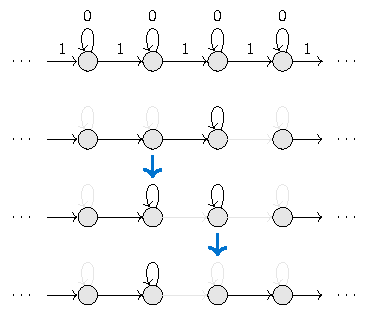
\includegraphics{figures/loop.pdf}
    %     \pgfmathsetmacro{\xdist}{1.1}
    % \pgfmathsetmacro{\ydist}{-1.2*\xdist}
        % \begin{tikzpicture}[
        %     scale=1, auto, node distance=1cm, 
        %     every edge/.style={draw, <-, looseness=20},
        %     state/.style={circle, fill=mylightgrey, draw=black, text=black},
        %     changebox/.style={draw=blue!70!black, very thick, rounded corners, inner sep=2pt}
        % ]
        
        % % -------------------------------------------------
        % % Row 0 : initial policy (all states choose move)
        % % -------------------------------------------------
        % % \node at (-2.2,  0.0) {$\pi^{(0)}$};
        % \node[font=\footnotesize] (l0) at (-\xdist, 0.0) {$\cdots$};
        
        % \node[state] (a1) at (0.0, 0.0) {};
        % \node[state] (a2) at (\xdist, 0.0) {};
        % \node[state] (a3) at (2*\xdist, 0.0) {};
        % \node[state] (a4) at (3*\xdist, 0.0) {};
        
        % \node[font=\footnotesize] (r0) at (4*\xdist, 0.0) {$\cdots$};
        
        % % move actions (active)
        % \draw[->] ($(l0.east)+(0.10,0)$) -- node[midway, above, font=\footnotesize] {$1$} (a1.west);
        % \draw[->] (a1.east) -- node[midway, above, font=\footnotesize] {$1$} (a2.west);
        % \draw[->] (a2.east) -- node[midway, above, font=\footnotesize] {$1$} (a3.west);
        % \draw[->] (a3.east) -- node[midway, above, font=\footnotesize] {$1$} (a4.west);
        % \draw[->] (a4.east) -- node[midway, above, font=\footnotesize] {$1$} ($(r0.west)+(-0.10,0)$);
        
        % % stay actions (inactive)
        % \path[->]
        %     (a1) edge[out=110, in=70, loop, looseness=12, draw=black]
        %         node[pos=0.5, above, text=black, font=\footnotesize] {$0$} (a1)
        %     (a2) edge[out=110, in=70, loop, looseness=12, draw=black]
        %         node[pos=0.5, above, text=black, font=\footnotesize] {$0$} (a2)
        %     (a3) edge[out=110, in=70, loop, looseness=12, draw=black]
        %         node[pos=0.5, above, text=black, font=\footnotesize] {$0$} (a3)
        %     (a4) edge[out=110, in=70, loop, looseness=12, draw=black]
        %         node[pos=0.5, above, text=black, font=\footnotesize] {$0$} (a4);
        
        % % \draw[->, dotted, thick]
        % %     ($(r0.south)+(0,-0.45)$)
        % %     to[out=0, in=-180, looseness=1]
        % %     ($(l0.south)+(0,-0.45)$);
        % % -------------------------------------------------
        % % Row 1 : state s_{i+1} switches to stay
        % % -------------------------------------------------
        % % \node at (-2.2, -1.9) {$\pi^{(1)}$};
        % \node[font=\footnotesize] (l1) at (-\xdist, \ydist) {$\cdots$};
        
        % \node[state] (b1) at (0.0, \ydist) {};
        % \node[state] (b2) at (\xdist, \ydist) {};
        % \node[state] (b3) at (2*\xdist, \ydist) {};
        % \node[state] (b4) at (3*\xdist, \ydist) {};
        
        % \node[font=\footnotesize] (r1) at (4*\xdist, \ydist) {$\cdots$};
        
        % % move actions
        % \draw[->] ($(l1.east)+(0.10,0)$) -- (b1.west);
        % \draw[->] (b1.east) -- (b2.west);
        % \draw[->] (b2.east) -- (b3.west);
        % \draw[->, draw=mylightgrey] (b3.east) -- (b4.west);
        % \draw[->] (b4.east) -- ($(r1.west)+(-0.10,0)$);
        
        % % stay actions
        % \path[->]
        %     (b1) edge[out=110, in=70, loop, looseness=12, draw=mylightgrey] (b1)
        %     (b2) edge[out=110, in=70, loop, looseness=12, draw=mylightgrey] (b2)
        %     (b3) edge[out=110, in=70, loop, looseness=12, draw=black] (b3)
        %     (b4) edge[out=110, in=70, loop, looseness=12, draw=mylightgrey] (b4);
        
        % % \node[changebox, fit=(b2)] (box1) {};
        
        % % -------------------------------------------------
        % % Row 2 : state s_{i+2} also switches to stay
        % % -------------------------------------------------
        % % \node at (-2.2, -1.9) {$\pi^{(1)}$};
        % \node[font=\footnotesize] (l2) at (-\xdist, 2*\ydist) {$\cdots$};
        
        % \node[state] (c1) at (0.0, 2*\ydist) {};
        % \node[state] (c2) at (\xdist, 2*\ydist) {};
        % \node[state] (c3) at (2*\xdist, 2*\ydist) {};
        % \node[state] (c4) at (3*\xdist, 2*\ydist) {};
        
        % \node[font=\footnotesize] (r2) at (4*\xdist, 2*\ydist) {$\cdots$};
        
        % % move actions
        % \draw[->] ($(l2.east)+(0.10,0)$) -- (c1.west);
        % \draw[->] (c1.east) -- (c2.west);
        % \draw[->, draw=mylightgrey] (c2.east) -- (c3.west);
        % \draw[->, draw=mylightgrey] (c3.east) -- (c4.west);
        % \draw[->] (c4.east) -- ($(r2.west)+(-0.10,0)$);
        
        % % stay actions
        % \path[->]
        %     (c1) edge[out=110, in=70, loop, looseness=12, draw=mylightgrey] (c1)
        %     (c2) edge[out=110, in=70, loop, looseness=12, draw=black] (c2)
        %     (c3) edge[out=110, in=70, loop, looseness=12, draw=black] (c3)
        %     (c4) edge[out=110, in=70, loop, looseness=12, draw=mylightgrey] (c4);
        
        % % \node[changebox, fit=(b2) (c2)] (box2) {};
        
        % % -------------------------------------------------
        % % Row 3 : state s_{i+3} also switches to stay
        % % -------------------------------------------------
        % % \node at (-2.2, -5.7) {$\pi^{(3)}$};
        % \node[font=\footnotesize] (l3) at (-\xdist, 3*\ydist) {$\cdots$};
        
        % \node[state] (d1) at (0.0, 3*\ydist) {};
        % \node[state] (d2) at (\xdist, 3*\ydist) {};
        % \node[state] (d3) at (2*\xdist, 3*\ydist) {};
        % \node[state] (d4) at (3*\xdist, 3*\ydist) {};
        
        % \node[font=\footnotesize] (r3) at (4*\xdist, 3*\ydist) {$\cdots$};
        
        % % move actions
        % \draw[->] ($(l3.east)+(0.10,0)$) -- (d1.west);
        % \draw[->] (d1.east) -- (d2.west);
        % \draw[->, draw=mylightgrey] (d2.east) -- (d3.west);
        % \draw[->] (d3.east) -- (d4.west);
        % \draw[->] (d4.east) -- ($(r3.west)+(-0.10,0)$);
        
        % % stay actions
        % \path[->]
        %     (d1) edge[out=110, in=70, loop, looseness=12, draw=mylightgrey] (d1)
        %     (d2) edge[out=110, in=70, loop, looseness=12] (d2)
        %     (d3) edge[out=110, in=70, loop, looseness=12, draw=mylightgrey] (d3)
        %     (d4) edge[out=110, in=70, loop, looseness=12, draw=mylightgrey] (d4);
        
        % % \node[changebox, fit=(c3) (d3)] (box3) {};
        
        % % -------------------------------------------------
        % % Blue arrows showing where the policy changes next
        % % -------------------------------------------------
        % % \draw[->, blue!70!black, very thick] (box1.south) -- (box2.north);
        % % \draw[->, blue!70!black, very thick] (box2.south) -- (box3.north);

        % \draw[->, very thick, CambridgeCoreBlue]
        %     ($(b2.south)+(0,-0.1)$) -- ($(c2.north)+(0,0.5)$);
        
        % \draw[->, very thick, CambridgeCoreBlue]
        %     ($(c3.south)+(0,-0.1)$) -- ($(d3.north)+(0,0.5)$);
        % \end{tikzpicture}
    \vspace{0.5cm}
    \caption{The MDP forms a connected chain of 13 states, each with two actions. 
    As in \autoref{fig: explain loop on-policy bias MDP}, solutions cycle between suboptimal policies that only contain 1 or 2 suboptimal actions.
    The suboptimal action propagates backwards relative to the state-transitions.}
    \label{fig: long MDP}
    \end{minipage}
    \hfill
    \begin{minipage}[b]{0.48\textwidth}
   % \begin{tikzpicture}
   %  \begin{axis}[
   %      width=\linewidth,
   %      height=5.4cm,
   %      % axis equal image,
   %      xmin=-0.007, xmax=0.0120,
   %      ymin=-0.02, ymax=0.0080,
   %      grid=none,
   %      grid style={line width=0.2pt, draw=gray!35},
   %      % major grid style={line width=0.3pt, draw=gray!45},
   %      tick label style={font=\small},
   %      title={Deterministic solution in $s_1$},
   %      xlabel={$q_k(s_1,a_*)-\widehat q$},
   %      ylabel={$q_k(s_1,\bar a)-\widehat q$},
   %      % legend style={draw=none, fill=none, font=\small, at={(0.65,.3)}, anchor=north},
   %      % legend columns=1,
   %      scaled ticks=true,
   %      every x tick scale label/.style={
   %          at={(axis description cs:1.0,0.0)},
   %          anchor=north,
   %          font=\small
   %      },
   %      every y tick scale label/.style={
   %          at={(axis description cs:0,1.0)},
   %          anchor=south,
   %          font=\small
   %      },
   %      % legend cell align={left}
   %      ]
   %      \addplot[forget plot, CambridgeCoreBlue]
   %          table[col sep=comma, x=x, y=y]{figures/deterministic_phase_path_s1.csv};
   %      % \addlegendentry{trajectory from CSV}
   %      \addplot[forget plot, only marks, mark=*, mark size=2.2pt, black]
   %          table[col sep=comma, x=x, y=y]{figures/spiral_initial_s1.csv}
   %          node[pos=0, right] {$q_0$};
   %      % \addlegendentry{initial}
   %      % \addplot+[forget plot, only marks, mark=x, mark size=3.0pt, line width=0.8pt]
   %      %     coordinates {(0,0)};
   %      % \addlegendentry{$(\widehat q,\widehat q)$}
   %      \addplot[forget plot, only marks, mark=square*, mark size=2.1pt]
   %          table[col sep=comma, x=x, y=y]{figures/spiral_final_s1.csv};
   %      % \addlegendentry{after 1000 cycles}
   %      \addplot[forget plot, dotted, black, domain=-0.010:0.02, samples=2] {x};
   %      % \addlegendentry{zero-gap line}
   %  \end{axis}
   %  \end{tikzpicture} 
   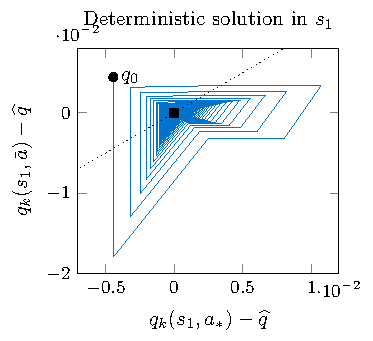
\includegraphics{figures/spiral-fig.pdf}
    \caption{Mean-field solutions of FV/SA MCES robustly converge to a suboptimal point $(\widehat q, \widehat q)$ derived in Appendix~\ref{sec:balance-general}.
    % Solutions
    % Deterministic expected-update spiral for state $s_1$. 
    Solution is initialised with counts $n_0(s,a_*):=10$ and $n_0(s,\bar a) := 5$.
    The dotted line corresponds to the boundary where $q(s_1,a_*)=q(s_1,\bar a)$}
    \label{fig:spiral}
    \end{minipage}
\end{figure}


% The designed cycle, for $N=14,$ uses a rotational family of starts, with one initial state/action pair $(s_{i+6}, \bar a)$ in the policies with a single stay at state $i$ (the "odd" policies $\pi_1$, $\pi_3$, $\pi_5$ for our earlier $N=3$ example in Figure~\ref{fig: explain loop on-policy bias MDP}). All state indices are to be taken modulo 14.  On the "even" policies, with adjacent stays at $\{s_i,s_{i+1}\}$, the process makes a sampled choice of $(s_{i-1}, \bar a)$ with probability $\lambda$ or $(s_{i+1}, a_*)$ with probability $(1-\lambda)$. At each timestep, with probability $\epsilon_{\mathrm{ES}}$ the designed choice of start is replaced by a uniform random choice amongst the 28 possible starts.

% Figure~\ref{fig:spiral} shows the evolution of $\mathbb E[q_{k+1}]$ under this rule when at each step $q_{k+1}$ and $n_{k+1}$ are replaced by their expected value. This behaviour is robust, in the sense that a large open set of initial conditions lead to solutions which spiral into the fixed point on boundary. The Appendix \ref{app: } shows that the point after one full cycle is a linear
% interpolation between the current point and the boundary point and thus that these policies are the only ones visited in the absence of noise.


% The fully sampled process is extremely noisy, 
% with stochastic returns due to the variable episode length and the sampled normal and exploring starts. 
% As a result the process frequently visits off cycle policies; 
% in this case a linear program is solved at each such step to choose a distribution of starts which points the process back towards the cycle. Exploring starts remain active during this recovery. Thus the sampling strategy is a memoryless function of the current $q_k$ (as would be the case for an $\epsilon$-greedy policy, for example) with a uniform lower bound on the probability of sampling any state/action pair at each step.

% The full sampled process is extremely noisy, with stochastic returns due to the variable episode length and the sampled normal and exploring starts. As a result the process frequently visits off cycle policies; in this case a linear program is solved at each such step to choose a distribution of starts which points the process back towards the cycle. Exploring starts remain active during this recovery. Thus the sampling strategy is a memoryless function of the current $q_k$ (as would be the case for an $\epsilon$-greedy policy, for example) with a uniform lower bound on the probability of sampling any state/action pair at each step.

% We systematically ran 33 simulations of the full FV/SA MCES sampled process for $\gamma=0.9999$, $\tau\approx 0.5088$ and 
% with exploring starts at the level of $\epsilon_{ES}=10^{-4}$ and found that, provided they survived an initial burn in, they converged towards a suboptimal point on the boundary.
% To be precise, 5 of the 33 simulations survived $10\times 10^6$ timesteps without escaping the boundary and, of these, 3 simulations survived a further $10\times 10^6$ timesteps. We continued these 3 for a further $10\times 10^6$ timesteps, a total $30\times 10^6$ timesteps, and all 3 survived.  We separately ran $100$ length $10^6$ simulations with the same parameters and a variety of seeds from the $k=20\times 10^6$ timestep of a long run and every one continued to converge to a suboptimal point on the boundary. Representative behaviour is shown in \autoref{fig:fvsasim}, and full details are provided in the Appendix.


Fully sampled FV/SA MCES solutions are extremely noisy, due to both sample returns and exploring starts.
As a result, they frequently visit off-cycle policies.
%\textcolor{red}{(suggestion)}
We then initialise episodes to 
guide the process back to an on-cycle policy as follows.
% Initial start pairs are then chosen to 
% guide the process back to a cycle policy as follows: 
On visiting the optimal all-"move" policy,
% the simulation chooses "stay" at the state for which the action-values are closest to the boundary as its initial condition.
we start episodes in the "stay" action of the state for which the action-values are closest to the boundary.
The first visit structure ensures that "move" is then also updated in that, and potentially downstream, states, 
and also that "move" actions are updated more often than "stay" actions overall. The $1/n_k(s,a)$ weighting then results in solutions being pushed towards and eventually across the boundary, creating a "stay" state.
% 
In all other off-cycle policies,
%\textcolor{red}{(suggestion)}
we first consider all states where "stay" is greedy and keep only those with the fewest neighbours that also prefer "stay". Among that subset, we choose the state whose action values are closest to the decision boundary, then initialize the episode in the "stay" action of that state.
% the simulation chooses "stay" at one of the states for which "stay" is greedy choosing, from the set with fewest "stay" neighbours, the one with action-values nearest the boundary. 
This eventually results in solutions crossing the boundary in the opposite direction, reducing the number of "stay" states until only a singleton or adjacent pair remain.   
%Full details are provided in Appendix~\ref{sec:recovery-strategy} 
Exploring starts remain active during the recovery.
The sampling strategy is thus completely determined by the current $q_k$ (as would be the case for an $\epsilon$-greedy policy, for example) with a uniform lower bound on the probability of sampling any state-action pair at each step.


We simulated $40,000$ solutions of FV/SA MCES with $\gamma=0.9999$, $\tau\approx 0.5123$ and $\epsilon_{ES}=10^{-4}$ for $10^9$ steps for a range of initial counts $n_k(s,\bar a)=M$, $n_k(s,a_*)=2.01M$ with $M$ from  $3000$ to $12000$ and found that all but a proportion of approximately $(2200/M)^{5.4}$ remained trapped in a shrinking strip around the boundary significantly below the optimal value. In each run, for approximately $14.9\%$ of steps the greedy policy was the all-"move" policy $\pi_*$ and for approximately $1.5\%$ of steps it was another off-cycle policy. Thus for a large majority of steps the system is in a cycle phase.       
For a representative sample of runs which hadn't escaped at $10^9$ steps we continued the simulation up to $10^{12}$ steps and none escaped. We then ran $8$ simulations from $M=10^5$ and all remained trapped at $10^{12}$ steps. That is, all trials that survived $10^9$ steps went on to survive $10^{12}$ steps. 
\autoref{fig:fvsasim} shows representative behaviour from a start at $M=1000$, demonstrating an initial lock in followed by the long $1/k$ tail.
%with further discussion in \autoref{app:fv}.
Altogether, these simulations provide strong evidence 
of high probability non-convergence to optimality from late starts of FV/SA MCES for this MDP; i.e.
that, for large $M$, starts from $n_k(s,\bar a)=M$ escape from the stable suboptimal basin with probability $O(M^{-K})\rightarrow 0$ for $K\approx 5.4$. 


\begin{figure}
    \centering
% \begin{subfigure}[b]{0.48\textwidth}
%     \includegraphics[width=\textwidth]{cyclefig}
%     \caption{Representative solution at early and intermediate times}
%     % \caption{$q_k(s,\bar a)$ vs $q_k(s,a_*)$ for a representative state at early and intermediate times}
%     \label{fig:cyclefig}
%     \end{subfigure}
%     \hfill
\begin{subfigure}[b]{0.48\textwidth}
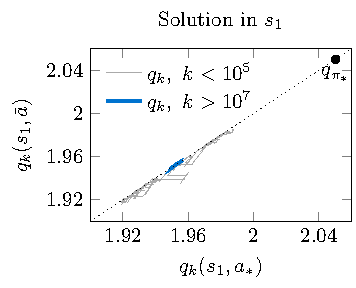
\includegraphics{figures/fv-simulation.pdf}
    % \begin{tikzpicture}
    %     \begin{axis}[
    %         width=0.9\linewidth,
    %         height=4.5cm,
    %         title={Solution in $s_1$},
    %         xmin=1.9, xmax=2.06,
    %         ymin=1.9, ymax=2.06,
    %         xlabel={$q_k(s_1,a_*)$},
    %         ylabel={$q_k(s_1,\bar a)$},
    %         xtick={1.92,1.96,2.00,2.04},
    %         ytick={1.92,1.96,2.00,2.04},
    %         legend style={
    %             draw=none,
    %             fill=none,
    %             at={(0.03,0.97)},
    %             anchor=north west
    %         },
    %         legend cell align={left},
    %         tick align=inside,
    %     ]
        
    %     % Early trajectory: q_k, k < 10^5
    %     \addplot+[
    %         mygrey,
    %         thin,
    %         mark=none
    %     ] table[
    %         x=q_star_action,
    %         y=q_bar_action,
    %         col sep=comma
    %     ] {figures/cycleplot_csv/q_early.csv};
    %     \addlegendentry{$q_k,\ k<10^5$}

    %     % \addplot+[
    %     %     blue,
    %     %     thin,
    %     %     mark=none
    %     % ] table[
    %     %     x=q_star_action,
    %     %     y=q_bar_action,
    %     %     col sep=comma
    %     % ] {figures/cycleplot_csv/q_early_late.csv};
    %     % \addlegendentry{{$q_k,\ k<10^5$}}
        
    %     % Boundary q_k(s,a_*) = q_k(s,\bar a)
    %     % \addplot+[
    %     %     red!60,
    %     %     dotted,
    %     %     thin,
    %     %     mark=none
    %     % ] table[
    %     %     x=q_star_action,
    %     %     y=q_bar_action,
    %     %     col sep=comma
    %     % ] {cycleplot_csv/boundary.csv};
    %     % \addlegendentry{boundary}
        
    %     % Optimal-policy value q_{\pi_*}
    %     % \addplot+[
    %     %     orange,
    %     %     only marks,
    %     %     mark=+,
    %     %     mark size=3pt,
    %     %     thick
    %     % ] table[
    %     %     x=q_star_action,
    %     %     y=q_bar_action,
    %     %     col sep=comma
    %     % ] {cycleplot_csv/q_pi_star.csv};
    %     % \addlegendentry{{$q_{\pi_*}$}}
        
    %     % Late trajectory: q_k, k > 10^7
    %     \addplot+[
    %         CambridgeCoreBlue,
    %         very thick,
    %         mark=none
    %     ] table[
    %         x=q_star_action,
    %         y=q_bar_action,
    %         col sep=comma
    %     ] {figures/cycleplot_csv/q_late.csv};
    %     \addlegendentry{{$q_k,\ k>10^7$}}

    %     \addplot[forget plot, dotted, black, domain=1.9:2.1, samples=2] {x};

    %     \addplot+[
    %         only marks,
    %         mark options={draw=black, fill=black},
    %         mark=*,
    %         mark size=2pt,
    %         % thick
    %     ] coordinates {(2.0504,2.0504)};
    %     \node[
    %         anchor=north
    %     ] at (axis cs:2.0504,2.0504) {$q_{\pi_*}$};
    %     \end{axis}
    %     \end{tikzpicture}
    \label{fig:cyclefig}
    \end{subfigure}
\hfill
\begin{subfigure}[b]{0.48\textwidth}
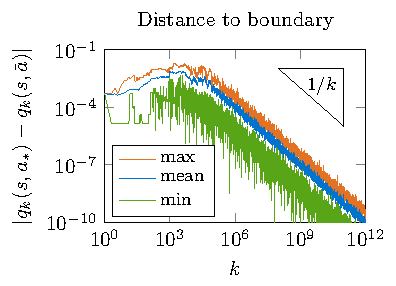
\includegraphics{figures/fv-contraction.pdf}
    % \begin{tikzpicture}
    %     \begin{axis}[
    %         width=0.9\linewidth,
    %         % height=.8\linewidth,
    %         % width=6cm,
    %         height=4.5cm,
    %         title={Distance to boundary},
    %         xmode=log,
    %         ymode=log,
    %         xmin=1,
    %         xmax=1e12,
    %         ymin=1e-10,
    %         ymax=1e-1,
    %         xtick ={1,10^(3),10^(6),10^(9),10^(12)},
    %         ytick distance=10^(3),
    %         xlabel={$k$},
    %         ylabel={$|q_k(s,a_*) - q_k(s,\bar a)|$},
    %         legend style={
    %             at={(0.03,0.03)},
    %             anchor=south west,
    %             draw=black,
    %             fill=white,
    %             font=\small
    %         },
    %         legend cell align={left},
    %         tick align=inside,
    %     ]
        
    %     \addplot+[
    %         CambridgeCoreOrange,
    %         thin,
    %         mark=none
    %     ] table[
    %         x=k,
    %         y=max_gap,
    %         col sep=comma
    %     ] {figures/cycleplot_csv/gap_stats.csv};
    %     \addlegendentry{max}

    %     \addplot+[
    %         CambridgeCoreBlue,
    %         thin,
    %         mark=none
    %     ] table[
    %         x=k,
    %         y=mean_gap,
    %         col sep=comma
    %     ] {figures/cycleplot_csv/gap_stats.csv};
    %     \addlegendentry{mean}
        
    %     \addplot+[
    %         CambridgeCoreGreen,
    %         thin,
    %         mark=none
    %     ] table[
    %         x=k,
    %         y=min_gap,
    %         col sep=comma
    %     ] {figures/cycleplot_csv/gap_stats.csv};
    %     \addlegendentry{min}
        
    %     % \addplot+[
    %     %     purple,
    %     %     thin,
    %     %     mark=none
    %     % ] table[
    %     %     x=k,
    %     %     y=ref_line,
    %     %     col sep=comma
    %     % ] {figures/cycleplot_csv/gap_stats.csv};
    %     % \addlegendentry{$0.1/k$}

    %     \draw[black] (axis cs:1e8, 1e-2) -- (axis cs:1e11, 1e-2) -- (axis cs:1e11,1e-5) -- cycle;
    %     \node[below left, font=\small] at (axis cs:1e11, 1e-2) {$1/k$};
    %     \end{axis}
    %     \end{tikzpicture}
\end{subfigure}
%     \hfill
% \begin{subfigure}[b]{0.48\textwidth}
%     \includegraphics[width=\textwidth]{gapfig}
%     \caption{gaps: $q_k(s,a_*)-q_k(s,\bar a)$}
%     \label{fig:gapfig}
% \end{subfigure}
\caption{First-visit MCES with sample-average updates can converge to a suboptimal solution where $q(s, a_*) = q(s, \bar a)$ for all states.}
\label{fig:fvsasim}
\end{figure}


\section{Conclusion}

We have presented two new counterexamples showing that both initial-visit and first-visit MCES can converge to suboptimal solutions, 
and proposed a practical fix that guarantees convergence to optimality in the initial-visit case.

Previous counterexamples for initial-visit MCES rely on sampling distributions that heavily favour non-greedy actions at every step.
% towards non-greedy actions at each step.
Our example shows that stable suboptimal solutions exist even when greedy actions are updated more frequently, as typically occurs during the exploitation phase.
The suboptimal behaviour arose because the sample-average learning rates introduced an effective bias towards non-greedy actions when solutions were in the optimal region.
% consistently driving solutions out of that region.
% This highlights that the asymptotic behaviour of MCES depends critically on the interplay between the learning rates and the update frequencies of actions within each state, rather than either factor alone.

% A simple learning-rate scheme restores convergence to optimality despite updating actions at different frequencies. 
We then presented a practical learning-rate scheme that restores convergence to optimality despite updating actions at different frequencies. 
% The key idea is to scale learning rates inversely with update frequencies on a state-by-state basis. This makes updates effectively uniform across actions within each state, causing the underlying mean-field to generate monotonically improving policies.
The key idea is to scale learning rates inversely with update frequencies on a state-by-state basis, so that the effective update size is uniform across actions within each state. Under this correction, the underlying mean-field generates monotonically improving policies. 
Since the stochastic perturbations cannot consistently prevent this improvement, initial-visit MCES eventually converges to the optimal policy and its action values.


Finally, we constructed a 13-state MDP in which first-visit MCES with sample-average updates converges to a suboptimal solution.
This example establishes that any convergence proof for first-visit MCES would need to show that solutions always escape suboptimal mean-field attractors.
In our simulations this occurs with sharply decreasing frequency for later starts, providing strong evidence that exploring starts alone do not guarantee convergence of Monte Carlo control methods to optimality.
% fundamental open question in reinforcement learning: 


% This highlights that the asymptotic behaviour of MCES depends critically on the interplay between the learning rates and the update frequencies of actions within each state, rather than either factor alone.
Overall, these results highlight that
the asymptotic behaviour of MCES depends critically on the interplay between learning rates and sampling distributions.
% the central issue when analysing MCES or implementing scalable variants is the interplay between learning rates and sampling distributions.
By controlling the frequency and magnitude of updates to each action, these parameters determine the effective update size.
Initial experiments (not presented here) suggest that MCES converges to optimality when, within each state, the effective update to the greedy action is at least as large as that to any other action.
Establishing this condition formally is an important direction for future work
as it may provide a foundation for analysing scalable MCES variants.



\clearpage
% \section*{References}
% \bibliographystyle{apalike}
\bibliographystyle{unsrt} % Use for unsorted references  
% \bibliographystyle{plainnat} % use this to have URLs listed in References
\bibliography{References/references} 


%%%%%%%%%%%%%%%%%%%%%%%%%%%%%%%%%%%%%%%%%%%%%%%%%%%%%%%%%%%%
\appendix
% \appendix
% Technical appendices with additional results, figures, graphs, and proofs may be submitted with the paper submission before the full submission deadline (see above). You can upload a ZIP file for videos or code, but do not upload a separate PDF file for the appendix. There is no page limit for the technical appendices. 

% Note: Think of the appendix as ``optional reading'' for reviewers. The paper must be able to stand alone without the appendix; for example, adding critical experiments that support the main claims to an appendix is inappropriate.
\newpage
\section{Counterexample for initial-visit MCES with non-greedy bias}
\label{app: non greedy}

Bertsekas and Tsitsiklis show in \cite[Example~5.12]{Bertsekas1996Neuro-DynamicProgramming} that IV MCES can converge to suboptimal solutions when greedy actions are updated less frequently than non-greedy actions.
The single-state MDP in \autoref{fig: experiment off-policy bias MDP} is the simplest such example.

Episodes are initialised to favour the non-greedy action,
meaning
when $q_k(s,\pi_*(s)) \ge q_k(s,\bar\pi(s))$
the initial state-action pair is $(s,\pi_*(s))$ with a small probability $\epsilon$ and $(s,\bar\pi(s))$ with probability $1-\epsilon$,
with the probabilities reversed otherwise.
% Alternatively, when
% $q_k(s,\pi_*(s)) < q_k(s,\bar\pi(s))$
% we initialise each episode in $(s,\pi_*(s))$ with probability $\epsilon$, or in $(s,\bar\pi(s))$ with probability $1-\epsilon$

\autoref{fig: experiment for off-policy bias} shows simulations with $\epsilon = 0.1$. The streamlines indicate the mean-field flow.
Solutions starting to the right of the separatrix typically converge to $q_{\pi_*}$, whereas those starting to the left leave the optimal region $Q(\pi_*)$ and converge to a boundary point.

% solutions which start in the region of the optimal policy, below the boundary, can leave it when to the left of the indicated separatrix, and converge to a point on the boundary which has the property that outflow and inflow are in opposite directions.   

\begin{figure}[htbp]
    \centering
    % \hrule
    % \vspace{0.4cm}

    \begin{subfigure}[b]{0.3\textwidth}
        \centering
        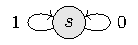
\includegraphics{figures/counter-mdp.pdf}
        % \begin{tikzpicture}[
        %     scale=1, auto, node distance=2cm, 
        %     every edge/.style={draw, <-, font=\small},
        %     state/.style={circle, fill=mylightgrey, draw=black, text=black}
        % ]
        %     % Nodes
        %     \node[state] (s1) at (0,0) {$s$};
        %     % Edges
        %     \path[->]
        %         (s1) edge[out=160, in=200, loop, looseness=8, draw=black] node[pos=0.5, left, text=black] {1} (s1)
        %         (s1) edge[out=20, in=340, loop, looseness=8, draw=black] node[pos=0.5, right, text=black] {0} (s1) ;
        %         % (s1) edge[out=145, in=215, loop, looseness=7] 
        %         %     node[pos=0.5, right] {$\best{a}$} 
        %         %     node[pos=0.5, left] {1} 
        %         % (s1)
        %         % (s1) edge[out=35, in=325, loop, looseness=7] 
        %         %     node[pos=0.5, left] {$\worst{a}$} 
        %         %     node[pos=0.5, right] {0} 
        %         % (s1);
        % \end{tikzpicture}
        \caption{MDP}
        \label{fig: mdp for unconditional experiment}
    \end{subfigure}%
    \hfill
    \begin{subfigure}[b]{0.3\textwidth}
        \centering
        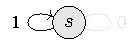
\includegraphics{figures/counter-mdp-opt.pdf}
        % \begin{tikzpicture}[
        %     scale=1, auto, node distance=2cm, 
        %     every edge/.style={draw, <-, font=\small},
        %     state/.style={circle, fill=mylightgrey, draw=black, text=black}
        % ]
        %     % Nodes
        %     \node[state] (s1) at (0,0) {$s$};
        %     % Edges
        %     \path[->]
        %         (s1) edge[out=160, in=200, loop, looseness=8, draw=black] node[pos=0.5, left, text=black] {1} (s1)
        %         (s1) edge[out=20, in=340, loop, looseness=8, draw=mylightgrey] node[pos=0.5, right, text=mylightgrey] {0} (s1) ;
        %         % (s1) edge[out=160, in=200, loop, looseness=8] node[pos=0.5, left] {$\begin{aligned}
        %         %     & \best{a} \\
        %         %     & 1
        %         % \end{aligned}$} (s1)
        %         % (s1) edge[out=20, in=340, loop, looseness=8, draw=mylightgrey] node[pos=0.5, right, text=mylightgrey] {$\begin{aligned}
        %         %     & \worst{a} \\
        %         %     & 0
        %         % \end{aligned}$} (s1);
        % \end{tikzpicture}
        \caption{Policy $\best{\pol}$}
    \end{subfigure}%
    \hfill
    \begin{subfigure}[b]{0.3\textwidth}
        \centering
        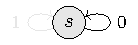
\includegraphics{figures/counter-mdp-worst.pdf}
        % \begin{tikzpicture}[
        %     scale=1, auto, node distance=2cm, 
        %     every edge/.style={draw, <-, font=\small},
        %     state/.style={circle, fill=mylightgrey, draw=black, text=black}
        % ]
        %     % Nodes
        %     \node[state] (s1) at (0,0) {$s$};
        %     % Edges
        %     \path[->]
        %         (s1) edge[out=160, in=200, loop, looseness=8, draw=mylightgrey] node[pos=0.5, left, text=mylightgrey] {1} (s1)
        %         (s1) edge[out=20, in=340, loop, looseness=8, draw=black] node[pos=0.5, right, text=black] {0} (s1) ;
        %         % (s1) edge[out=160, in=200, loop, looseness=8, draw=mylightgrey] node[pos=0.5, left, text=mylightgrey] {$\begin{aligned}
        %         %     & \best{a} \\
        %         %     & 1
        %         % \end{aligned}$} (s1)
        %         % (s1) edge[out=20, in=340, loop, looseness=8] node[pos=0.5, right] {$\begin{aligned}
        %         %     & \worst{a} \\
        %         %     & 0
        %         % \end{aligned}$} (s1);
        % \end{tikzpicture}
        \caption{Policy $\worst{\pol}$}
    \end{subfigure}%
    
    \caption{MDP that exhibits a stable suboptimal solution for IV MCES when updates are biased towards non-greedy actions.}
    \label{fig: experiment off-policy bias MDP}
\end{figure}

\begin{figure}[htbp]
    \centering
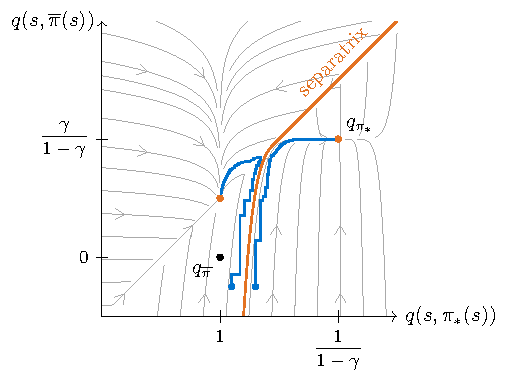
\includegraphics{figures/simple-counter.pdf}
   %  \pgfmathsetmacro{\ticklen}{0.1}
   %  \pgfmathsetmacro{\xmin}{-1}
   %  \pgfmathsetmacro{\xmax}{4}
   %  \pgfmathsetmacro{\ymin}{-1}
   %  \pgfmathsetmacro{\ymax}{4}
    
   %  \pgfmathsetmacro{\qbpolx}{3}
   %  \pgfmathsetmacro{\qbpoly}{2}
   %  \pgfmathsetmacro{\qwpolx}{1}
   %  \pgfmathsetmacro{\qwpoly}{0}

    
   % %\begin{subfigure}[b]{0.9\textwidth}
   % %    \centering

   %      \begin{tikzpicture}[scale=1]

   %          \pgfmathsetmacro{\eps}{0.9}
   %          \pgfmathsetmacro{\mbpolx}{1-\eps}
   %          \pgfmathsetmacro{\mbpoly}{\eps}
   %          \pgfmathsetmacro{\mwpolx}{\eps}
   %          \pgfmathsetmacro{\mwpoly}{1-\eps}
        
   %          \pgfmathsetmacro{\qc}{(\mbpolx*\qbpolx - \mbpoly*\qbpoly)/(\mbpolx - \mbpoly)}
        
   %          % Add the streamline plot using pgfplots
   %          \begin{axis}[
   %              hide axis,
   %              xmin=\xmin, xmax=\xmax,
   %              ymin=\ymin, ymax=\ymax,
   %              width=5cm, % Scale the width to match your scaling
   %              height=5cm, % Adjust for aspect ratio
   %              clip=true, % Hide parts of streamlines outside the axes
   %              scale only axis,
   %              xshift=-1cm, % Custom shift in x-direction
   %              yshift=-1cm % Custom shift in y-direction
   %          ] 
   %              \addplot[mygrey, no marks] 
   %              table [ x expr=\thisrowno{0}, 
   %                      y expr=\thisrowno{1}, 
   %                      col sep=comma, 
   %                      unbounded coords=jump] 
   %              {figures/32/streamlines-strong-off-policy.csv};

   %              \addplot[CambridgeCoreBlue, no marks, line width=0.3mm] 
   %              table [ x expr=\thisrowno{0}, 
   %                      y expr=\thisrowno{1}, 
   %                      col sep=comma, 
   %                      unbounded coords=jump] 
   %              {figures/32/simulations-strong-off-policy.csv};
    
   %              \addplot[
   %                  smooth,
   %                  line width=0.3mm,
   %                  CambridgeCoreOrange,
   %                  domain=-4:0,
   %                  samples=10
   %              ] plot ( 
   %                  {\qc + (1 - exp(-\mbpolx*x)) * (\qbpolx - \qc)}, 
   %                  {\qc + (1 - exp(-\mbpoly*x)) * (\qbpoly - \qc)}
   %              );
   %              \addplot[
   %                  smooth,
   %                  line width=0.3mm,
   %                  CambridgeCoreOrange,
   %                  domain=0:1,
   %                  samples=2
   %              ] plot ( 
   %                  {x*\qc + (1 - x) * \xmax}, 
   %                  {x*\qc + (1 - x) * \ymax}
   %              );
   %          \end{axis}
    
   %          % Draw the grid and axes
   %          \draw[->] (\xmin,\ymin) -- (\xmax,\ymin) node[right] {$q(s,\best{\pol}(s))$};
   %          \draw[->] (\xmin,\ymin) -- (\xmin,\ymax) node[left] {$q(s,\worst{\pol}(s))$};
   %          % \draw (\xmin,\ymax) -- (\xmax,\ymax) ;
   %          % \draw (\xmax,\ymin) -- (\xmax,\ymax) ;
    
   %          % Draw the line y = x
   %          % \draw[black, dotted] (\xmin,\ymin) -- (\xmax,\ymax);
    
   %          % Add labels to the axes
   %          \draw (\qbpolx,\ymin+\ticklen) -- (\qbpolx,\ymin-\ticklen) node[below, font=\small] {$\dfrac{1}{1-\discount}$};
   %          \draw (\xmin+\ticklen,\qbpoly) -- (\xmin-\ticklen,\qbpoly) node[left, font=\small] {$\dfrac{\discount}{1-\discount}$};
   %          \draw (\qwpolx,\ymin+\ticklen) -- (\qwpolx,\ymin-\ticklen) node[below, font=\small] {$1$};
   %          \draw (\xmin+\ticklen,\qwpoly) -- (\xmin-\ticklen,\qwpoly) node[left, font=\small] {0};
    
   %          % Add the points with associated text
   %          \filldraw[fill=CambridgeCoreOrange, draw=CambridgeCoreOrange] (\qbpolx,\qbpoly) circle (1.5pt) node[above right, text=black] {$q_{\best{\pol}}$};
   %          \filldraw[fill=black, draw=black] (\qwpolx,\qwpoly) circle (1.5pt) node[below left, text=black] {$q_{\worst{\pol}}$};
   %          \filldraw[fill=CambridgeCoreOrange, draw=CambridgeCoreOrange] (\qwpolx,\qwpolx) circle (1.5pt) ;
   %          \filldraw[fill=CambridgeCoreBlue, draw=CambridgeCoreBlue] (1.2, -0.5) circle (1.5pt) ;
   %          \filldraw[fill=CambridgeCoreBlue, draw=CambridgeCoreBlue] (1.6, -0.5) circle (1.5pt) ;
   %          \node at (\xmax-0.25,\ymax-0.25) [anchor=south east, rotate=45, text=CambridgeCoreOrange] {separatrix};
    
   %      \end{tikzpicture}
    %\end{subfigure}%
    % \vspace{0.3cm}
    \caption{The streamlines of the mean-field flow indicate that there are two basins of attraction when the non-greedy bias is large ($\epsilon = 0.1$).
    Solutions starting to the left of the separatrix tend to converge to a suboptimal fixed point on the boundary when the learning rates are sufficiently small.
    Those starting to the right converge to $\qopt$. The two simulations of MCES in blue confirm this conclusion.}
    \label{fig: experiment for off-policy bias}
        \label{fig: experiment for off-policy bias large}
\end{figure}

\section{Proof of \autoref{thm: iv mcopi with 1/g scaling}}
\label{app: proof of stochastic theorem}

%%%%%%%%%%%%%%%%%%%%%%%%%%%%%%%%%%%%%%%%%%%%%%%%%%%%%%
%%%%%%%%%%%%%%%%%%%%%%%%%%%%%%%%%%%%%%%%%%%%%%%%%%%%%%
% \subsection{Difference equation}

% \autoref{thm: iv mcopi with 1/g scaling} is essentially an application of the following result.

% \begin{theorem}
% \label{thm: iv mcopi converges as}
% Assume the sampling distributions $\{\sigma_k\}_{k \ge 0}$ are uniform over the actions in each state:
% \begin{align}
% \label{eq: uniform sampling}
% % \sigma_k(s,a) = \sigma_k(s,a')
% \sigma_k(s,a) = \frac{f_k(s)}{|\aset(s)|},
% \qquad 
% \forall \, k \ge 0, \
% \forall \, s \in \sset, \
% \forall \, a \in \aset(s) .
% \end{align}
% % for every time $k \ge 0$, every state $s \in \mathcal S$, and all actions $a, a' \in \mathcal A(s)$.
% Under \autoref{asp: standing}, solutions of IV MCES \eqref{eq: update iv mcopi} converge almost surely to $q_{\pi_*}$.
% \end{theorem}

% This appendix proves \autoref{thm: iv mcopi converges as} 
% and then shows that the same proof applies to \autoref{thm: iv mcopi with 1/g scaling}



Define the perturbation $v_k := \tilde q_k - q_{\pi_k}$ where $\tilde q_k$ is the episode return defined in \eqref{eq: episode return},
as well as the indicator $u_k(s, a) := \mathbf{1}_{\{(s,a)=(s_k,a_k)\}}$ that captures the randomness of asynchronous updates.
Combine these two sources of noise into a single stochastic perturbation $w_k$ defined as
\begin{align}
\label{eq: noise definition appendix}
w_k(s,a) 
&:=
\frac{1}{g_k(a | s)}
\Big( u_k(s,a) v_k(s,a)
+
\big( u_k(s,a) - \sigma_k(s,a) \big) \big( q_{\pi_k}(s,a) - q_k(s,a) \big) \Big) .
\end{align}
Equation \eqref{eq: update iv mcopi} with learning rates as in \eqref{eq: normalised learning rates} is then equivalent, for every state-action pair, to
\begin{align}
% \label{eq: intermediate stochastic step}
\nonumber
q_{k+1}(s,a)
&=
q_k(s,a) + \alpha_k \frac{u_k(s,a)}{g_k(a | s)} \big( q_{\pi_k}(s,a) + v_k(s,a) - q_k(s,a) \big)
\\
\label{eq: stochastic rep of normalised}
    &=
    q_k(s,a) + \alpha_k \big( f_k(s) ( q_{\pi_k}(s,a) - q_k(s,a) ) + w_k(s,a) \big) 
\end{align}
where $\pi_k$ is a deterministic policy that is greedy with respect to $q_k$.
% The sequence $\{\pi_k\}_{k \ge 0}$ thus remains in the finite set of deterministic policies, denoted $\mathcal P$.

\autoref{thm: iv mcopi with 1/g scaling} is an adaptation of Proposition~20 in \cite{Oliviers2026ConvergenceUpdates}. The event construction and policy-improvement argument are unchanged: 
stochastic perturbations cannot consistently undermine the policy improvement driven by the mean-field dynamics,
so $\pi_k$ eventually stabilises at $\pi_*$ and $q_k \to q_{\pi_*}$.


The only modification is the normalized learning rate $\alpha_k/g_k(a\mid s)$ in place of $\alpha_k$. Since $g_k(a\mid s) \in (0,1]$, this rescaling is positive and at least as large as $\alpha_k$, so the induction in Lemma~15 is unaffected. Lemmas~17 and~18 require only that $w_k$ is a martingale difference sequence with bounded second moment; this is verified in the lemma below.



% While several standard frameworks can derive the convergence of a stochastic difference inclusion from the corresponding mean-field dynamics, they each face structural limitations
% when applied to MC-O-PI.

% As hinted in the proof sketch, the convergence argument consists of showing that the stochastic perturbations $\{w_k\}_{k \ge 0}$ cannot consistently prevent the mean-field policy improvement.
% As a result, the policy sequence eventually reaches the optimal policy $\pi_*$ and solutions converge to its action values $q_{\pi_*}$.
% So we start by deriving fundamental properties of these perturbations.
% Unless stated otherwise, operations and relations between functions are elementwise. For instance, given functions $f, g : \xset \to \yset$ we write
% \begin{align}
% &(f + g)(x) = f(x) + g(x), \qquad \forall \, x \in \xset ,
%     \\
% &f \le g \iff f(x) \le g(x), \qquad \forall \, x \in \xset .
% \end{align}
% Furthermore, every norm is computed as $\|f\| := \sup_{x \in \xset} |f(x)|$.
% % The stochastic perturbations $w_k$ sat

% %%%%%%%%%%%%%%%%%%%%%%%%%%%%%%%%%%%%%%%%%%%%%%%%%%%%%%
% %%%%%%%%%%%%%%%%%%%%%%%%%%%%%%%%%%%%%%%%%%%%%%%%%%%%%%
% % \subsection{Basic properties}

\begin{lemma}
% [Martingale difference noise]
\label{thm: properties of noise}
% Under initial- or first-visit updates, 
There exists a constant $c_w \in [0, \infty)$ 
such that
\begin{align}
\label{eq: condition on combined noise for proof}
\mathbb E[w_k(s,a) \mid \mathcal F_k] = 0,
\ \ \
\mathbb E[w_k^2(s,a) \mid \mathcal F_k] \le c_w(1+\|q_k\|^2),
\ \ \
\forall \, k \ge 0, \,
\forall \, s \in \mathcal S, \,
\forall \, a \in \mathcal A(s) .
\end{align}
% for every time $k \ge 0$, every state $s \in \sset$ and every action $a \in \aset(s)$,
% \begin{align}
% \label{eq: muw_mds}
% &\E\!\left[w_k(s,a) \mid \mathcal F_k\right] = 0,
% \\
% \label{eq: muw_second_moment}
% &\E\!\left[w_k^2(s,a) \mid \mathcal F_k\right]
% \le c_w(1+\|q_k\|^2) .
% \end{align}
\end{lemma}
\begin{proof}
Fix a time $k\ge 0$, a state $s \in \mathcal S$ and an action $a \in \mathcal A(s)$.
Let $\mathcal F_k'$ represent the available information right after selecting the policy $\pi_k$ but before sampling the initial state-action pair $(s_k, a_k)$, so $\mathcal F_k \subseteq \mathcal F_k'$.

Under initial-visit updates, $\tilde q_k$ is an unbiased estimate of $q_{\pi_k}$ with uniformly bounded variance
\cite{Singh1996ReinforcementTraces}.
Thus there exists a constant $c_v \in [0,\infty)$ such that
\begin{align}
\label{eq: properties episode noise}
\mathbb E\!\left[v_k(s,a) \mid \mathcal F_k \right] = 0 ,
\qquad
\mathbb E\!\left[v_k^2(s,a) \mid \mathcal F_k \right] \le c_v,
\qquad
\forall \, k \ge 0 .
\end{align}
Further, 
% $\mathbb E[u_k(s,a) \mid \mathcal F_k] = \sigma_k(s,a) = f_k(s) g_k(a | s)$ under initial-visit updates, 
% and 
$u_k(s,a) v_k(s,a) = 0$ on $\{u_k(s,a)=0\}$.
Hence,
\begin{align}
\label{eq: noise unbiased part 1}
\mathbb E\big[ u_k(s,a) v_k(s,a) \mid \mathcal F'_k \big]
=
\mathbb E \Big[ 
    \mathbf{1}_{\{u_k(s,a)=1\}} \ 
    \mathbb E \big[ v_k(s,a) \mid \mathcal F'_k, u_k(s,a) = 1 \big]
    \mid \mathcal F'_k \Big]
    = 0 .
\end{align}
Also,
$\E[u_k(s,a) \mid \mathcal F'_k] = \sigma_k(s,a)$ 
and
% given that $k$, $s$ and $a$ are fixed,
$\sigma_k(s,a)$ and $(q_{\pi_k}(s,a)-q_k(s,a))$ are $\mathcal F'_k$-measurable. It follows that
\begin{multline}
\mathbb E \!\left[ 
\big( u_k(s,a) - \sigma_k(s,a) \big) \big( q_{\pi_k}(s,a) - q_k(s,a) \big)
\mid \mathcal F'_k
\right]
\\
\label{eq: noise unbiased part 2}
=
\big(
\mathbb E [ u_k(s,a) \mid \mathcal F'_k ]
- \sigma_k(s,a)
\big)
\big( q_{\pi_k}(s,a)-q_k(s,a) \big)
=
0 .
\end{multline}
Since $g_k(a | s)$ is $\mathcal F'_k$-measurable,
dividing \eqref{eq: noise unbiased part 1} and \eqref{eq: noise unbiased part 2} by $g_k(a | s)$ and summing the results yields $\mathbb E[w_k(s,a) \mid \mathcal F'_k] = 0$.
Applying the tower property then gives
\begin{align}
\label{eq: noise is unbiased}
\mathbb E [ w_k(s,a) \mid \mathcal F_k ]
= \mathbb E \big[ \mathbb E [ w_k(s,a) \mid \mathcal F'_k] \mid \mathcal F_k \big]
= 0 .
\end{align}

Finally,
$g_k^2(a | s) \ge \sigma_{\min}^2$ by the strict exploring starts condition in \eqref{eq: strict exploring starts},
% $|\mathcal A(s)| \ge \min_{s} |\mathcal A(s)| =: |\mathcal A_{\min}|$,
$u_k^2(s,a) \le 1$ 
and $(u_k(s,a) - \sigma_k(s,a))^2 \le 1$ for every state-action pair.
Using $(x+y)^2 \le 2 x^2 + 2 y^2$ on \eqref{eq: noise definition appendix} thus yields
\begin{align*} 
w_k^2(s,a) 
&\le
\frac{1}{\sigma_{\min}^2} \big( 2 v_k^2(s,a) + 2 (q_{\pi_k}(s,a)-q_k(s,a) )^2 \big)
\\
&\le
\frac{1}{\sigma_{\min}^2} \big( 2 v_k^2(s,a) + 4 q_{\pi_k}^2(s,a) + 4 q_k^2(s,a) \big) .
\end{align*}
Since all action-values are bounded,
there exists a constant $c_\polset \in [0,\infty)$ such that $\|q_\pi\|^2 \leq c_\polset$ for every policy $\pi$. 
As a result, using \eqref{eq: properties episode noise} yields
\begin{align}
\nonumber
\mathbb E \!\big[ w_k^2(s,a) \mid \mathcal F_k \big]
% &\le
% \frac{1}{\sigma_{\min}^2 |\mathcal A_{\min}|^2}  \left( 2 c_v + 2 \, \mathbb E \!\left[ ( q_{\pi_k}(s,a)-q_k(s,a) )^2 \mid \mathcal F_k \right] \right)
% \\
% % \label{eq: noise has bounded variance}
% \nonumber
&\le
\frac{2}{\sigma_{\min}^2} ( c_v + 2 c_\polset + 2 \|q_k\|^2 ) .
\\
\label{eq: noise has bounded variance}
&\le
\max\left\{ \frac{2}{\sigma_{\min}^2} ( c_v + 2 c_\polset), \frac{4}{\sigma_{\min}^2} \right\} ( 1 + \|q_k\|^2 ) .
\end{align}
Equations \eqref{eq: noise is unbiased} and \eqref{eq: noise has bounded variance} confirm that the perturbations $\{w_k\}_{k \ge 0}$ satisfy the conditions in \eqref{eq: condition on combined noise for proof}.
\end{proof}

% %%%%%%%%%%%%%%%%%%%%%%%%%%%%%%%%%%%%%%%%%%%%%%%%%%%%%%
% %%%%%%%%%%%%%%%%%%%%%%%%%%%%%%%%%%%%%%%%%%%%%%%%%%%%%%
% % \subsection{Bounded solutions}

% Given these properties of $w_k$, 
% we can apply standard martingale and stochastic approximation arguments to establish fundamental properties of \eqref{eq: stochastic rep of normalised}.
% For instance, if the target action values $q_{\pi_k}$ were fixed,
% solutions would converge almost surely to this fixed target by Proposition~4.1 or Example~4.3 in \cite{Bertsekas1996Neuro-DynamicProgramming}.
% As a result, solutions of the switched system are almost surely bounded.


% \begin{lemma}
% % [Bounded limit set]
% \label{thm: bounded limit sets}
% Consider the setting of \autoref{thm: iv mcopi with 1/g scaling}.
% Let $\polset_\infty$ denote the set of policies that appear infinitely often in a sequence $\{\pi_k\}_{k \ge 0}$ generated by \eqref{eq: stochastic rep of normalised}.
% % \begin{align}
% %     \polset_\infty \coloneqq \bigcap_{t = 0}^{\infty} \text{cl} \{\pi_k : k \geq t \} ,
% % \end{align}
% The corresponding sequence $\{q_k\}_{k \ge 0}$ converges almost surely to the set
% \begin{align*}
%     \Big\{
%     q : 
%     \min_{\pi \in \polset_\infty} q_\pi(s,a) \leq q(s,a) \leq \max_{\pi \in \polset_\infty} q_\pi(s,a), \forall s \in \sset, \forall a \in \aset(s)
%     \Big\} .
% \end{align*}
% % Consequently,
% % Let $\{q_k\}_{k\ge 0}$ be a solution of \eqref{eq: iv mcopi in stochastic theorem}.
% % There exists an almost surely finite constant $c_Q \in [0, \infty)$ such that for all $k \geq 0$
% % \begin{align*}
% %     \| q_k \|_\infty^2 < c_Q .
% % \end{align*}
% \end{lemma}

% \begin{proof}
% Let $\{q_k\}_{k \ge 0}$ and $\{\pol_k\}_{k \ge 0}$ be solutions of \eqref{eq: stochastic rep of normalised} with initial condition $q_0$, learning rates $\{\alpha_k\}_{k \ge 0}$, state-sampling distributions $\{f_k\}_{k \ge 0}$ and stochastic perturbations $\{w_k\}_{k \ge 0}$.
    
% By assumption, there exists a finite time $K$ such that
% the sequence $\{\pol_k\}_{k \ge K}$ only contains policies in $\polset_\infty$.
% % the estimate $q_k$ is updated towards action values $q_{\pi_k}$ where $\pi_k \in \polset_\infty$.
% Thus for all $k \ge K$, each state-action pair $(s,a)$ of the estimate $q_k$ is updated towards a value $q_{\pol_k}(s,a)$ that satisfies
% \begin{align}
%     \min_{\pi \in \polset_\infty} q_\pi(s,a) \leq q_{\pi_k}(s,a) \leq \max_{\pi \in \polset_\infty} q_\pi(s,a) .
% \end{align}
% Therefore, define the sequences $\{x_k\}_{k \ge K}$ and $\{y_k\}_{k \ge K}$ as
% \begin{align}
%     x_\kpo &= x_k + \alpha_k 
%     \left(
%     % \sigma_k(s,a) 
%     f_k(s) \bigg( \min_{\pi \in \polset_\infty} q_\pi(s,a) - x_k \bigg) + w_k(s,a) \right) ,
%     \\
%     y_\kpo &= y_k + \alpha_k 
%     \left(
%     % \sigma_k(s,a) 
%     f_k(s) \bigg( \max_{\pi \in \polset_\infty} q_\pi(s,a) - y_k \bigg) + w_k(s,a) \right) ,
% \end{align}
% and initialised at $x_K = y_K = q_K(s,a)$. From time $K$ onwards we have
% \begin{align*}
%     x_k \leq q_k(s,a) \leq y_k .
% \end{align*}
% Standard results show that $x_k$ and $y_k$ converge almost surely to $\min_{\pi \in \polset_\infty} q_\pi(s,a)$ and $\max_{\pi \in \polset_\infty} q_\pi(s,a)$, respectively~\citep[Proposition~4.1, Example~4.3]{Bertsekas1996Neuro-DynamicProgramming}.
% % , because the noise satisfies conditions \eqref{eq: muw_mds} and \eqref{eq: muw_second_moment}.
% As a result, we conclude that, almost surely,
% \begin{align*}
%     \liminf_{k \to \infty} q_k(s,a)
%     \ge \min_{\pi \in \polset_\infty} q_\pi(s,a) ,
%     % \leq q_k(s,a) 
%     \quad
%     \limsup_{k \to \infty} q_k(s,a)
%     \le \max_{\pi \in \polset_\infty} q_\pi(s,a) ,
%     \quad
%     \forall \, s \in \sset , \
%     \forall \, a \in \aset(s) .
% \end{align*}
% % for every state-action pair.
% \end{proof}

% %%%%%%%%%%%%%%%%%%%%%%%%%%%%%%%%%%%%%%%%%%%%%%%%%%%%%%
% %%%%%%%%%%%%%%%%%%%%%%%%%%%%%%%%%%%%%%%%%%%%%%%%%%%%%%
% % \subsection{Policy transitions}

% Furthermore, given solutions would converge almost surely to $q_{\pi_k}$ if these values were fixed in \eqref{eq: stochastic rep of normalised},
% the asymptotic behaviour of \eqref{eq: stochastic rep of normalised} hinges on how these action values evolve over time.
% To isolate these changes, we introduce \emph{transition times}.
% We adopt the convention $\inf \varnothing = \infty$.

% \begin{definition}
% \label{def: transition times}
% Given a sequence of policies $\{\pi_k\}_{k \ge 0}$,
% define the transition times $\{t_n\}_{n \ge 0}$ as
% \begin{align*}
% t_0 \coloneqq 0 ,
% \qquad
% t_{n+1} \coloneqq \inf\{k>t_n : q_{\pi_k} \neq q_{\pi_{t_n}} \} .
% \end{align*}
% % with the convention that $\inf \varnothing = \infty$.
% Thus, if $t_n = \infty$, then $t_{n+i} = \infty$ for all $i \ge 1$ .
% These times decompose the sequence $\{\pi_k\}_{k \ge 0}$ into blocks of constant action values, such that $q_{\pi_k} = q_{\pi_{t_n}}$ for all $k \in \{t_n, \dots, t_{n+1}-1 \}$.
% \end{definition}

% % Clearly, if $\pi_{t_n}$ is suboptimal, then $t_{n+1}<\infty$.
% % Otherwise the target would remain equal to \(q_{\pi_{t_n}}\) forever, forcing convergence to \(q_{\pi_{t_n}}\).
% % However a suboptimal policy is not greedy with respect to its own action values.
% % Thus no solution can get arbitrarily close to $q_{\pi_{t_n}}$ without causing the greedy policy to improve. Therefore no suboptimal block can persist indefinitely.

% \begin{lemma}
% \label{thm: suboptimal blocks finite}
% If $\pi_{t_n}$ is not optimal, then $t_{n+1}<\infty$ almost surely.
% \end{lemma}
% \begin{proof}
% Let $\pi := \pi_{t_n}$.
% Suppose for contradiction that $t_{n+1}=\infty$. The target in \eqref{eq: stochastic rep of normalised} is then fixed at $q_\pi$ forever, and $q_k \to q_\pi$ almost surely by Proposition~4.1 in \cite{Bertsekas1996Neuro-DynamicProgramming}.
% However, since $\pi$ is suboptimal, it is not greedy with respect to $q_\pi$. Thus there exists a state-action pair $(s,a)$ such that $q_\pi(s,a) > q_\pi(s,\pi(s))$.
% As a result, as $q_k$ approaches $q_\pi$,
% every greedy policy $\pi_k$ with respect to $q_k$ satisfies
% $q_\pi(s,\pi_k(s)) > q_\pi(s,\pi(s))$
% for all sufficiently large $k$.
% The Policy Improvement Theorem then indicates that $q_{\pi_k} \ne q_\pi$, contradicting $t_{n+1}=\infty$.
% \end{proof}

% % 
% % Consequently, if there exists a finite index $n$ such that $t_{n} = \infty$, the associated solution converges to the action values of the last bounded transition time, which must be optimal.
% % Conversely, any suboptimal asymptotic behaviour requires an infinite sequence of bounded transition times.


% We rely on the following strict version of the of the Policy Improvement Theorem at transition times.
% \begin{lemma}
% \label{thm: strict improvement theorem}
% Given policies \(\pi,\pi'\in\mathcal P\), suppose
% \begin{align}
% \label{eq: PIT condition}
% q_\pi(s,\pi'(s)) \ge q_\pi(s,\pi(s))
% \qquad \forall s\in\mathcal S .
% \end{align}
% Then \(v_{\pi'} \ge v_\pi\). Moreover, if \(q_{\pi'}\neq q_\pi\), then the improvement is strict:
% there exists a state \(s\in\mathcal S\) where
% \[
% v_{\pi'}(s)>v_\pi(s).
% \]
% \end{lemma}
% \begin{proof}
% By the Policy Improvement Theorem, inequality \eqref{eq: PIT condition} implies that $v_{\pi'} \ge v_\pi$.
% Suppose that $v_{\pi'} = v_{\pi}$. Then for every state-action pair $(s,a)$,
% \begin{align*}
% q_{\pi'}(s,a)
% = r(s,a) + \gamma \sum_{s' \in \mathcal S} p (s' \mid s,a) v_{\pi'}(s')
% = r(s,a) + \gamma \sum_{s' \in \mathcal S} p (s' \mid s,a) v_{\pi}(s')
% = q_{\pi}(s,a) .
% \end{align*}
% As a result, if $q_{\pi'} \neq q_\pi$, there exists at least one state $s$ where $v_{\pi'}(s) > v_{\pi}(s)$, implying that policy $\pi'$ is better than $\pi$.
% \end{proof}


% %%%%%%%%%%%%%%%%%%%%%%%%%%%%%%%%%%%%%%%%%%%%%%%%%%%%%%
% %%%%%%%%%%%%%%%%%%%%%%%%%%%%%%%%%%%%%%%%%%%%%%%%%%%%%%
% \subsection{Lower bound on the probability of policy improvement at transitions}

% Consider the sequences $\{q_k\}_{k\ge 0}$ and $\{\pi_k\}_{k\ge 0}$ generated by \mcopi, and let $\{t_n\}_{n \ge 0}$ be the associated transition times.
% Over each interval $\{t_n, \dots, t_{n+1}\}$, we compare the evolution of $q_{k}$ at $(s,\pi_{t_n}(s))$ and pairs $(s,a)$ that would worsen the policy $\pi_{t_n}$, namely
% \[
% \mathcal B_{\pi_{t_n}} := \big\{ (s,a) : s \in \mathcal S, \ a \in \mathcal A(s), \ q_{\pi_{t_n}}(s,a) < q_{\pi_{t_n}}(s, \pi_{t_n}(s)) \big\} .
% \]
% % We build an event that guarantees that, 
% We show that, with a fixed probability and for sufficiently large $n$,
% for every $k \in \{t_n, \dots, t_{n+1}\}$
% the greedy policy satisfies $(s, \pi_k(s)) \notin \mathcal B_{\pi_{t_n}}$.
% % either $(s, \pi_{t_{n+1}}(s)) \notin \mathcal B_{\pi_{t_n}}$ for every state $s$,
% % or $t_{n+1} = \infty$.
% % The first case implies that
% % \begin{align}
% % \label{eq: goal of proof stoch improvement}
% % q_{\pi_{t_n}} ( s, \pi_{t_{n+1}}(s) )
% % \ge
% % q_{\pi_{t_n}} ( s,\pi_{t_n}(s) )
% % \end{align}
% % and therefore that the policy $\pi_{t_{n+1}}$ is better than $\pi_{t_n}$ by \autoref{thm: strict improvement theorem}.
% % The second case means that, by \autoref{thm: suboptimal blocks finite}, $\pi_{t_n} = \pi_*$ and thus $q_k$ will converge to the associated optimal action values.
% % Overall, either the policy improves, or it is already optimal and stays optimal.
% As a result, if $t_{n+1}<\infty$ we obtain
% \begin{align}
% \label{eq: goal of proof stoch improvement}
% q_{\pi_{t_n}} ( s, \pi_{t_{n+1}}(s) )
% \ge
% q_{\pi_{t_n}} ( s,\pi_{t_n}(s) )
% \end{align}
% and therefore policy $\pi_{t_{n+1}}$ is better than $\pi_{t_n}$ by \autoref{thm: strict improvement theorem}.
% Or if $t_{n+1} = \infty$,
% \autoref{thm: suboptimal blocks finite} implies that $\pi_{t_n} = \pi_*$ and $q_k$ converges to the associated optimal action values.
% In other words, the policy either improves, or it is already optimal and stays optimal.


% % By \autoref{def: transition times}, the target action values are fixed at $q_{\pi_{t_n}}$ for all times $ k \in \{t_n,\dots,t_{n+1}-1\}$.
% % We know that if $\pi_{t_n}$ is suboptimal then $t_{n+1}$ is almost surely finite, and hence $\pi_{t_{n+1}}$ is well defined.
% % The following result establishes a uniform lower bound on the probability that policy $\pi_{t_{n+1}}$ is better than $\pi_{t_{n}}$.

% % Technically, discounted or episodic MDPs can have several optimal policies.
% % We denote the set of all such optimal policies by $\mathcal P_*$. By definition, all optimal policies share the same value functions, denoted $v_{\best{\pi}}$ and $q_{\best{\pi}}$.
% % Furthermore, at least one policy in $\mathcal P_*$ is deterministic.

% % The main point to proving \autoref{thm: fixed prob that bad actions dont become greedy} is to construct a nonzero-probability event that ensures that


% \begin{proposition}
% \label{thm: fixed prob that bad actions dont become greedy}
%     Let $\{\pi_k\}_{k\ge 0}$ be a sequence of policies generated by
%     system \eqref{eq: stochastic rep of normalised}
%     under the setting of \autoref{thm: iv mcopi with 1/g scaling}.
%     Let $\{t_n\}_{n\ge 0}$ be the associated transition times.
%     There exist a constant $p>0$ and an almost surely finite time $K$ such that
%     for every $n \in \mathbb Z_{\ge 0}$ with $K \le t_n < \infty$,
%     \begin{align}
%     \label{eq: porb better action value}
%     \mathbb P \big(
%     \forall \, s \in \sset, \
%     \forall \, k \in \{t_n, \dots , t_{n+1} \}
%     \ : \
%     (s, \pi_k(s)) \notin \mathcal B_{\pi_{t_n}}
%     \mid \mathcal F_{t_n}
%     \big) \ge p .
%     \end{align}
% \end{proposition}


% We track the distance between $(s,\pi_{t_n}(s))$ and pairs in $\mathcal B_{\pi_{t_n}}$ using gap variables.

% \begin{definition}[Gap variables]
% \label{def: gap variables}
% % Let $\{t_n\}_{n\ge 0}$ be the transition times associated with the policy sequence generated by system \eqref{eq: stochastic rep} under the setting of \autoref{thm: iv mcopi converges as}.
% Fix a finite transition index $n \in \mathbb Z_{\ge 0}$
% and write $\pi := \pi_{t_n}$.
% % For each state $s \in \mathcal S$ and action $a \in \mathcal A(s)$, the gap is initialised at time $t_n$ as
% For each $k \in \{t_n, \dots, t_{n+1}\}$, define
% \begin{align*}
% % \label{eq: def gap initialisation}
% % d_{t_n}(s,a) = q_{t_n}(s,\pi(s)) - q_{t_n}(s,a) ,
% d_{k}(s,a) = q_{k}(s,\pi(s)) - q_{k}(s,a) .
% \end{align*}
% While $k < t_{n+1}$, each gap evolves as
% \begin{align}
% \label{eq: def gap evolution}
% d_{k+1}(s,a) = d_k(s,a) + \alpha_k \left( f_k(s)(d_\pi(s,a) - d_k(s,a)) + \xi_k(s,a) \right)
% \end{align}
% % where we used
% % \begin{align*}
% %     \mu_k(s) \coloneqq 
% %     % \sigma_k(s,\pi(s)) = \sigma_k(s,a) = 
% %     \frac{f_k(s)}{|\aset(s)|},
% % \end{align*}
% with the target gap
% \begin{align*}
% % \label{eq: def policy gap}
%     d_\pi(s,a) \coloneqq q_{\pi}(s,\pi(s)) - q_{\pi}(s,a) ,
% \end{align*}
% and the gap noise
% \begin{align*}
% % \label{eq:xi-def}
%     \xi_k(s,a) &\coloneqq
% w_{k}(s,\pi(s)) - w_{k}(s,a) .
% % \\
% % \nonumber
% % &\: = u_k(s,\pi(s))v_k(s,\pi(s)) - u_k(s,a) v_k(s,a)
% % \\
% % \nonumber
% % &\: \quad + \bigl( u_k(s,\pi(s)) - \mu_k(s) \bigr) \bigl( q_\pi(s,\pi(s)) - q_k(s,\pi(s)) \bigr)
% % \\
% % \nonumber
% % &\: \quad - \bigl( u_k(s,a) - \mu_k(s) \bigr) \bigl( q_\pi(s,a) - q_k(s,a) \bigr) .
% \end{align*}
% \end{definition}

% % Note that we are not saying that the policy does not change between $t_n$ and $t_{n+1}-1$. Instead we just say that it does not matter because the target action values remain fixed and, as long as we can guarantee that no action from $\mathcal B_{\pi_{t_n}}$ is sampled during that time frame that is enough, i.e.
% % \[
% % q_{k}(s,\pi_k(s)) \ge q_{k}(s,\pi_{t_n}(s)) \ge q_{k}(s,a)
% % \]

% % Even though $w_k(s,\pi(s))$ and $w_k(s,a)$ are not independent, the gap noise $\xi_k(s,a)$ is unbiased and its conditional variance is eventually bounded by a constant.

% \begin{lemma}
% \label{thm: properties noise gap}
% There exist a constant $c_\xi \in [0,\infty)$ 
% % such that for every \mcopi{} solution there is 
% and an almost surely finite time $K_\xi$ such that
% for every transition index $n \in \mathbb Z_{\ge 0}$ satisfying $t_n \ge K_\xi$,
% \begin{align*}
% % \label{eq:xi-mean}
% \mathbb E [ \xi_{k}(s,a) \mid \mathcal F_k ] = 0 ,
% % \\
% % \label{eq:xi-var}
% \quad
% \mathbb E [ \xi_{k}^2(s,a) \mid \mathcal F_k ] \le c_\xi ,
% \quad
% \forall \, k \in \{t_n, \dots, t_{n+1}-1\}, \
% \forall \, s \in \mathcal S, \
% \forall \, a \in \mathcal A(s) .
% \end{align*}
% % for every $k \in \{t_n, \dots, t_{n+1}-1\}$, every $s \in \mathcal S$, and every $a \in \mathcal A(s)$.
% % For every time $k \ge 0$,
% % every state $s \in \mathcal S$,
% % and every action $a \in \mathcal A(s)$,
% % \begin{align}
% % \label{eq:xi-mean}
% % &\mathbb E\!\left[ \xi_{k}(s,a) \mid \mathcal F_k \right] = 0 .
% % \end{align}
% % Moreover, there exists a constant $c_\xi>0$ 
% % % such that for every \mcopi{} solution there is 
% % and an almost surely finite time $K_\xi$ such that
% % for every time $k \ge K_\xi$,
% % every state $s \in \mathcal S$,
% % and every action $a \in \mathcal A(s)$,
% % \begin{align}
% % \label{eq:xi-var}
% % &\mathbb E\!\left[ \xi_{k}^2(s,a) \mid \mathcal F_k \right] \le c_\xi .
% % \end{align}
% \end{lemma}
% \begin{proof}
% \autoref{thm: properties of noise}
% % requires that $w_k(s,a)$ is unbiased.
% directly yields
% \[
% \E\!\big[ \xi_{k}(s,a) \mid \mathcal F_k \big] 
% =
% \E\!\big[ w_{k}(s,\pi_{t_n}(s)) \mid \mathcal F_k \big] - \E\!\big[ w_{k}(s,a) \mid \mathcal F_k \big] 
% = 
% 0 .
% \]

% Further,
% \autoref{thm: bounded limit sets} implies that
% % $q_k$ converge almost surely to the set $\bigl\{ q \in \mathcal Q : q_{\worst{\pi}} \le q \le q_{\best{\pi}} \bigr\}$, where $\overline \pi$ and $\pi_*$ are the worst and best policies of the MDP, respectively.
% % Thus, 
% there exists an almost surely finite time $K_{\xi}$ such that $\| q_k \| \le c_{\mathcal P} + 1$ for every $k \ge K_{\xi}$,
% with $c_{\mathcal P} := \max_{\pi}\| q_\pi \|_\infty$.
% Substituting this into \eqref{eq: condition on combined noise for proof} yields
% \[
% \mathbb E[w_k^2(s,a) \mid \mathcal F_k] 
% \le c_w(1+\|q_k\|^2)
% \le c_w(1+(c_{\mathcal P} + 1)^2)
% \qquad
% \forall \, k \ge K_{\xi}, \
% \forall \, s \in \mathcal S, \
% \forall \, a \in \mathcal A(s).
% \]
% Using $(x-y)^2 \le 2 ( x^2 + y^2)$ then shows that,
% % proves
% % \eqref{eq:xi-var}
% for every $k \ge K_{\xi}$, every $s \in \mathcal S$, and all $a, a' \in \mathcal A(s)$,
% \begin{align*}   
% \mathbb E\!\left[ \bigl(w_k(s,a) - w_k(s,a') \bigr)^2 \ \big| \ \mathcal F_k \right]
% &\le
% 2 \left( \mathbb E\!\left[ w_k^2(s,a) \mid \mathcal F_k \right] 
% + \mathbb E\!\left[ w_k^2(s,a') \mid \mathcal F_k \right] \right)
% \\
% &\le
% 4 \, c_w \left( 1 + (c_{\mathcal P}+1)^2 \right)
% =: c_\xi .
% \end{align*}
% % for every $k \ge K$, every $s \in \mathcal S$, and all $a, a' \in \mathcal A(s)$.
% % Hence, \eqref{eq:xi-var} holds with $c_\xi := 4 \, c_w \left( 1 + (c_{\mathcal P}+1)^2 \right)$ and $K_\xi = K$.
% \end{proof}


% % We show that, since each gap is non-negative at initialisation because $\pi_{t_n}$ is greedy with respect to $q_{t_n}$,
% % and (2) the target $d_{\pi_{t_n}}$ is strictly positive for each pair in $\mathcal B_{\pi_{t_n}}$,
% % there is a fixed probability that no pair in $\mathcal B_{\pi_{t_n}}$ is greedy at time $t_{n+1}$, and hence that we obtain \eqref{eq: goal of proof stoch improvement}.

% Over each interval $\{t_n, \dots, t_{n+1}\}$,
% we construct three events that guarantee that the gap $d_k$ of each pair in $\mathcal B_{\pi_{t_n}}$ is strictly positive up to time $t_{n+1}$,
% and consequently that no such pair is greedy.
% Specifically, we fix a margin $\delta>0$.
% The \textit{seed} event $\mathcal E^s_{t_n}$ first forces each gap at least up to $O(\alpha_k)$.
% The \textit{growth} event $\mathcal E^g_{t_n}$ then drives each gap from $O(\alpha_k)$ to $\delta$.
% Finally, the \textit{lock-in} event $\mathcal E^l_{t_n}$ ensures that after reaching $\delta$, each gap remains strictly positive up to time $t_{n+1}$.


% Concretely, define the minimum target gap across all policies
% \[
% d_{\min}
% \coloneqq
% \min_{\pi\in\mathcal P}\ \inf_{(s,a)\in \mathcal B_\pi} d_\pi(s,a) > 0 .
% \]
% % with the convention that $\min\varnothing=\infty$.
% Using the constants $\sigma_{\min}$ and $\rho_\alpha$ from
% \eqref{eq: strict exploring starts}--\eqref{eq: comparability of learning rates},
% we choose $\delta$ such that
% \begin{equation}
% \label{eq:delta-choice}
% 0<\delta<\min\left\{\frac{d_{\min}}{8},\,\frac{\rho_\alpha \sigma_{\min} d_{\min}}{32}\right\}.
% \end{equation}
% This allows us to define the constants
% \begin{align}  
% \label{eq:c-def}
% % \label{eq:cs-def}
% c_s \coloneqq \left( \frac{d_{\min}}{4} - \delta \right) > 0,
% % \\
% % \label{eq:cg-def}
% \quad
% c_g \coloneqq \sigma_{\min} ( d_{\min} - 2 \delta) > 0,
% % \\
% % \label{eq:c-def}
% \quad
% c \coloneqq \min \left\{ c_s, c_g \right\} > 0.
% \end{align}


% %%%%%%%%%%%%%%%%%%%%%%%%%%%%%%%%%%%%%%%%%%%%%%%%%%%%%%%%%%%%%%%
% \paragraph{Seed event pushes gap up to $\bm{O(\alpha_k)}$.}

% Let $M \in \mathbb N$ denote a finite time horizon whose value will be fixed later.
% For any time $k \in \{t_n, \ldots, t_{n+1}-1\}$, we define the seed event differently if the value of the greedy action is under- or overestimated.
% % Concretely, for any index $n \in \mathbb Z_{\ge 0}$,
% % any time $k \in \{t_n, \dots, t_{n+1}-1\}$,
% % any state $s \in \mathcal S$,
% % and any action $a \in \mathcal A(s)$,
% Namely, if $q_{\pi_{t_n}}(s,\pi_{t_n}(s)) - q_{k}(s,{\pi_{t_n}}(s)) \ge d_{\min}/2$,
% we update the pair $(s,{\pi_{t_n}}(s))$ for $M$ consecutive steps and require that the noise at each step is not too negative. We gather these conditions in the event
% \begin{align*}
%     \mathcal E^+_k(s,a)
%     \coloneqq 
%     \bigcap_{k'=k}^{k+M-1}
%     \left\{
%     u_{k'}(s,\pi_{t_n}(s)) = 1, \
%     v_{k'}(s,\pi_{t_n}(s)) \ge -\frac{d_{\min}}{4}
%     \right\} .
% \end{align*}
% On the other hand, if $q_{\pi_{t_n}}(s,\pi_{t_n}(s)) - q_{k}(s,{\pi_{t_n}}(s)) < d_{\min}/2$,
% we update $(s,a)$ and require that the noise is not too positive:
% \begin{align*}
%     \mathcal E^-_k(s,a)
%     \coloneqq 
%     \bigcap_{k'=k}^{k+M-1}
%     \left\{
%     u_{k'}(s,a) = 1, \
%     v_{k'}(s,a) \le \frac{d_{\min}}{4}
%     \right\} .
% \end{align*}
% Altogether, we obtain the seed event
% \begin{multline}
% \label{eq: def good prefix}
%     \mathcal E^s_k(s,a) \coloneqq 
%     \left( \left\{ q_{\pi_{t_n}}(s,\pi_{t_n}(s)) - q_{k}(s,{\pi_{t_n}}(s)) \ge \frac{d_{\min}}{2} \right\} \cap \mathcal E^+_k(s,a) \right) 
%     \\
%     \bigcup 
%     \left( \left\{ q_{\pi_{t_n}}(s,\pi_{t_n}(s)) - q_{k}(s,\pi_{t_n}(s)) < \frac{d_{\min}}{2} \right\} \cap \mathcal E^-_k(s,a) \right) .
% \end{multline}
% We also define the hitting time
% \[
% \tau^s_k(s,a) \coloneqq \inf \big\{ k' \in \{k+1, \dots, k+M \} : q_{k'}(s,\pi_{t_n}(s))-q_{k'}(s,a) \ge \delta \} ,
% \]
% and the accumulated learning rate mass between times $k$ and $k'>k$ as
% \[
% A(k,k') \coloneqq \sum_{i=k}^{k'-1} \alpha_{i} .
% \]
% % with the convention that $A(k, k) = 0$.
% We now show that, on $\mathcal E^s_k(s,a)$, ``bad'' gaps grow at least up to $O(\alpha_k)$ in $M$ steps.

% \begin{lemma}[Seed event]
% \label{thm: event to reach a_k margin}
% Consider the setting of \autoref{thm: fixed prob that bad actions dont become greedy}.
% For every index $n \in \mathbb Z_{\ge 0}$,
% every pair $(s,a) \in \mathcal B_{\pi_{t_n}}$
% and every time $k \in \{t_n, \dots, t_{n+1}-1\}$,
% the joint event
% \begin{align}
% \label{eq: joint seed event}
% \mathcal E^s_k(s,a)
% \cap
% % \big\{0 \leq q_{k}(s,\pi_{t_n}(s)) - q_{k}(s,a) < \delta \big\}
% \big\{0 \leq d_k(s,a) < \delta \big\}
% \end{align}
% guarantees that 
% % for every $k'$ satisfying 
% % % $k < k' \le \big( \tau^s_k(s,a) \wedge (k+M) \wedge t_{n+1} \big)$,
% % $k < k' \le \min\{ \tau^s_k(s,a), k+M, t_{n+1} \}$,
% \begin{align}
% \label{eq: lower bound during good prefix}
%     d_{k'}(s,a)
%     % q_{k'}(s,\pi_{t_n}(s)) - q_{k'}(s,a)
%     > c_s A(k,k') > 0
%     \qquad 
%     \forall \, k < k' \le \min\{ \tau^s_k(s,a), k+M, t_{n+1} \} .
% \end{align}
% % for every $k'$ that satisfies $k < k' \le \big( \tau^s_k(s,a) \wedge (k+M) \wedge t_{n+1} \big)$.
% Moreover, 
% % the probability of $\mathcal E^s_k(s,a)$ is lower bounded by
% \begin{align}
% \label{eq: probability reach a_k margin}
%     \mathbb P ( \mathcal E^s_k(s,a) \mid \mathcal F_k, \pi_{t_n} ) \ge \left( \sigma_{\min} \frac{d_{\min}^2}{d_{\min}^2 + 16 c_v} \right)^M > 0 .
% \end{align}
% \end{lemma}

% \begin{proof}
% Fix a transition index $n \in \mathbb Z_{\ge 0}$ and let $\pi := \pi_{t_n}$.
% Fix a pair $(s,a) \in \mathcal B_\pi$,
% define the sequence $\big\{ d_k(s,a) \big\}_{k=t_n}^{t_{n+1}}$ as in \autoref{def: gap variables}, and write $d_k := d_k(s,a)$ and $d_\pi := d_\pi(s,a)$ for brevity.
% Fix a time $k \in \{t_n, \dots, t_{n+1}-1\}$ and write $\tau^s_k := \tau^s_k(s,a)$.

% % We split the proof along the two mutually exclusive cases that make up $\mathcal E^s_k(s,a)$.


% When $q_\pi(s,\pi(s)) - q_{k}(s,\pi(s)) \ge d_{\min}/2$,
% % On 
% event $\mathcal E^+_k(s,a)$
% % only $(s, \pi(s))$ is updated.
% % during $M$ consecutive steps,
% % and $v_{k'}(s,\pi(s)) \ge -d_{\min}/4$ for every $k' \in \{k, \dots, k+M-1\}$.
% implies that for every $k'$ satisfying
% % $k \le k' < \big((k+M) \wedge t_{n+1} \big)$,
% $k \le k' < \min\{ k+M, t_{n+1} \}$,
% \begin{align}
% \nonumber
%     d_{k'+1}
%     &= d_{k'} + 
%     % \alpha_{k'} 
%     \frac{\alpha_{k'}}{g_{k'}(\pi(s) | s)}
%     \big( q_\pi(s,\pi(s)) - q_{k'}(s,\pi(s)) + v_{k'}(s,\pi(s)) \big)
%     \\
% \label{eq: plug noise into update of seed stage case 1}
%     &\ge d_{k'} + 
%     % \alpha_{k'} 
%     \frac{\alpha_{k'}}{g_{k'}(\pi(s) | s)}
%     \left( q_\pi(s,\pi(s)) - q_{k'}(s,\pi(s)) - \frac{d_{\min}}{4} \right) .
% \end{align}
% Given that $0 \le d_{k} < \delta$ and $d_{k'} < \delta$ while $k'< \tau^s_k$,
% it follows that 
% \begin{align}
% % \nonumber
% \label{eq: lower bound update step in seed stage case 1}
%     q_\pi(s,\pi(s)) - q_{k'}(s,\pi(s))
%     = q_\pi(s,\pi(s)) - d_{k'} + d_{k} - q_{k}(s,\pi(s))
%     % \\
%     > \frac{d_{\min}}{2} - \delta > 0
% \end{align}
% as long as
% % $k \le k' < \big( \tau^s_k \wedge (k+M) \wedge t_{n+1} \big)$,
% $k \le k' < \min\{ \tau^s_k , k+M, t_{n+1} \}$.
% Equations \eqref{eq: plug noise into update of seed stage case 1} and \eqref{eq: lower bound update step in seed stage case 1}
% thus indicate that, on \eqref{eq: joint seed event},
% % for every $k'$ satisfying
% % $k \le k' < \min\{ \tau^s_k , k+M, t_{n+1} \}$,
% % the gap strictly increases at each time $k'$ in the restricted range:
% \begin{align}
% \label{eq: final lower bound case 1}
%     d_{k'+1}
%     > d_{k'} +
%     \alpha_{k'}
%     \left( \frac{d_{\min}}{4} - \delta \right)
%     = d_{k'} + \alpha_{k'} c_s
%     % > 0 .
%     \qquad
%     \forall \, k \le k' < \min\{ \tau^s_k , k+M, t_{n+1} \} .
% \end{align}

% Similarly, when $q_\pi(s,\pi(s)) - q_{k}(s,\pi(s)) < d_{\min}/2$
% % event $\mathcal E^-_k(s,a)$ guarantees that
% % only $(s, a)$ is updated during $M$ consecutive steps, and $v_{k'}(s,a) \le d_{\min}/4$ for every $k' \in \{k, \dots, k+M-1\}$.
% we obtain
% \begin{align}
% % \nonumber
%     d_{k'+1}
%     % &= d_{k'} + \alpha_{k'}(q_{k'}(s,a) - q_\pi(s,a) - v_{k'}(s,a))
%     % \\
% \label{eq: plug noise into update of seed stage case 2}
%     &\ge d_{k'} + 
%     % \alpha_{k'} 
%     \frac{\alpha_{k'}}{g_{k'}(a | s)}
%     \left( q_{k'}(s,a) - q_\pi(s,a) - \frac{d_{\min}}{4} \right)
% \end{align}
% as long as
% % $k \le k' < \big((k+M) \wedge t_{n+1} \big)$,
% $k \le k' < \min\{ k+M, t_{n+1}\}$.
% Since $q_{k}(s,\pi(s))$ is unchanged on $\mathcal E^-_k(s,a)$
% and $d_{k'} < \delta$ while $k' < \tau^s_k$,
% it follows that
% \begin{align}
% % \nonumber
%     q_{k'}(s,a) - q_\pi(s,a)
%     = d_\pi - \big( q_\pi(s,\pi(s)) - q_{k}(s,\pi(s)) \big) - d_{k'}
%     % \\
% \label{eq: lower bound update step in seed stage case 2}
%     % > d_{\min} - \frac{d_{\min}}{2} - \delta
%     % \ge \frac{d_{\min}}{2} - \delta 
%     > \frac{d_{\min}}{2} - \delta
%     > 0
% \end{align}
% as long as
% % $k \le k' < \big( \tau^s_k \wedge (k+M) \wedge t_{n+1} \big)$,
% $k \le k' < \min\{ \tau^s_k, k+M, t_{n+1} \}$.
% Hence \eqref{eq: plug noise into update of seed stage case 2} and \eqref{eq: lower bound update step in seed stage case 2} confirm that, on \eqref{eq: joint seed event},
% % the gap strictly increases at each time $k'$ in the restricted range:
% \begin{align}
% \label{eq: final lower bound case 2}
%     d_{k'+1}
%     > d_{k'} + 
%     \alpha_{k'}
%     \left( \frac{d_{\min}}{4} - \delta \right)
%     = d_{k'} + \alpha_{k'} c_s
%     % > 0 .
%     \qquad
%     \forall \, k \le k' < \min\{ \tau^s_k , k+M, t_{n+1} \} .
% \end{align}
% By induction on \eqref{eq: final lower bound case 1} or \eqref{eq: final lower bound case 2},
% % and shifting the index by 1 to include time step $k'+1$,
% we obtain
% \begin{align}
% \label{eq: increase in d^b case B}
%     d_{k'}
%     > d_{k} + c_s A(k,k')
%     \ge c_s A(k,k') > 0
%     \qquad
%     \forall \, k < k' \le \min\{ \tau^s_k , k+M, t_{n+1} \} .
% \end{align}
% % for every $k'$ satisfying
% % $k < k' \le \min\{ \tau^s_k , k+M, t_{n+1} \}$,
% % as long as $k < k' \le \big( \tau^s_k \wedge (k+M) \wedge t_{n+1} \big)$, 
% which proves \eqref{eq: lower bound during good prefix}.

% Finally, 
% % we lower-bound the probability of $\mathcal E^s_k(s,a)$.
% given that $v_k$ is unbiased and its variance is bounded by $c_v$ uniformly over the policies,
% Cantelli's inequality implies that for every $k' \ge 0$, every $s \in \mathcal S$ and every $a \in \mathcal A(s)$,
% \begin{align}
% &\mathbb P \! \left( v_{k'}(s,a) \ge -\frac{d_{\min}}{4} \,\middle|\, \mathcal F_{k'}, u_{k'}(s,a)=1 \right) \ge \frac{d_{\min}^2}{d_{\min}^2 + 16 c_v},
% \label{eq:noise-lower}
% \\
% &\mathbb P \! \left( v_{k'}(s,a) \le \frac{d_{\min}}{4} \,\middle|\, \mathcal F_{k'}, u_{k'}(s,a)=1 \right) \ge \frac{d_{\min}^2}{d_{\min}^2 + 16 c_v}.
% \label{eq:noise-upper}
% \end{align}
% Since the case choice in \eqref{eq: def good prefix} is measurable on $\{\mathcal F_{k}, \pi_{t_n}\}$ and the minimum sampling probability of any state-action pair is $\sigma_{\min}$ by \eqref{eq: strict exploring starts},
% % under strict exploring starts,
% repeated conditioning over $M$ steps yields
% \begin{align}
% \label{eq: prob of good prefix}
% \mathbb P \big( \mathcal E^s_k(s,a) \mid \mathcal F_{k} , \pi_{t_n} \big) \ge \left( \sigma_{\min} \frac{d_{\min}^2}{d_{\min}^2 + 16 c_v} \right)^M > 0 .
% \end{align}
% Since $n$, $(s,a)$ and $k$ were chosen arbitrarily from their respective sets, the result holds uniformly.
% \end{proof}

% %%%%%%%%%%%%%%%%%%%%%%%%%%%%%%%%%%%%%%%%%%%%%%%%%%%%%%%%%%%%%%%
% \paragraph{Growth event pushes gap from $\bm{O(\alpha_k)}$ to $\bm{\delta}$}

% % Let $N(k)$ denote the minimum number of steps required to accumulate a particular amount of learning rate mass:
% Define the growth window $N(k)$ as
% \begin{align}
% N(k)
% % \coloneqq
% % \inf \left\{ i \ge 1 : 
% % A(k,k+i)
% % \ge \frac{4 \delta}{c_g} \right\} .
% \:=
% \left\lceil \frac{4 \delta}{c_g \rho_\alpha \alpha_k} \right\rceil . 
% \end{align}

% \begin{lemma}
% \label{thm: growth window}
% % Under condition \eqref{eq: comparability of learning rates},
% There exists a finite time $K_N$ such that for every $k \ge K_N$,
% \[
% N(k) \le \frac{1}{\alpha_{k}},
% \qquad 
% A(k,k + N(k)) \ge \frac{4 \delta}{c_g} .
% \]
% \end{lemma}
% \begin{proof}
% The definitions of $\delta$ and $c_g$ in \eqref{eq:delta-choice}--\eqref{eq:c-def} ensure that
% \begin{multline*}
%     \frac{4 \delta}{c_g \rho_\alpha}
%     < 
%     \frac{4 \rho_\alpha \sigma_{\min} d_{\min}}{32 \sigma_{\min}(d_{\min} - 2 \delta) \rho_\alpha}
%     =
%     \frac{d_{\min}}{8 (d_{\min} - 2 \delta)}
% %    \\
%     <
%     \frac{d_{\min}}{8(d_{\min} - d_{\min}/4)}
%     =
%     \frac{1}{6}
%     < 1 .
% \end{multline*}
% The Robbins--Monro conditions in \eqref{eq: robbins monro conditions} imply that $\alpha_k \to 0$. So there exists a finite $K$ such that $4\delta / c_g \rho_\alpha + \alpha_k < 1$ for all $k \ge K$,
% and hence
% \[
% N(k) < \frac{4 \delta}{c_g \rho_\alpha \alpha_k} + 1 < \frac{1}{\alpha_k} .
% \]
% % Let
% % \[
% % r_k := \left\lceil \frac{4 \delta}{c_g \rho_\alpha \alpha_k} \right\rceil .
% % \]
% % Since $r_k \le 1/ \alpha_k$,
% The comparability property of the learning rates in \eqref{eq: comparability of learning rates} then guarantees that $A(k, k+N(k)) \ge N(k) \rho_\alpha \alpha_{k} \ge 4 \delta / c_g$ for every $k \ge K_n := \max\{K, K_\alpha\}$.
% % \[
% % A(k, k+r_{k}) \ge r_{k} \rho_\alpha \alpha_{k} \ge 4 \delta / c_g .
% % \]
% % As a result, there exists a finite time $K_N \ge \max\{K, K_\alpha\}$ such that $N(k) \le r_k \le 1/\alpha_{k}$ for all $k \ge K_N$.
% \end{proof}

% For any $k \in \{t_n, \dots, t_{n+1}-1\}$,
% % any state $s \in \mathcal S$
% % and any action $a \in \mathcal A(s)$,
% define the accumulated stochastic perturbations between $k$ and $k'>k$ as
% \[
% \Xi(k, k' \mid s,a) 
% \coloneqq 
% \sum_{i=k}^{k'-1} \alpha_{i} \xi_i(s,a)
% =
% \sum_{i=k}^{k'-1} \alpha_{i} \big( w_i(s, \pi_{t_n}(s))-w_i(s,a) \big) ,
% \]
% % with the convention $\Xi(k, k \mid s,a) = 0$.
% define the growth event
% % For any index $n \in \mathbb Z_{\ge 0}$,
% % any time $k \in \{t_n, \dots, t_{n+1}-1\}$,
% % any state $s \in \mathcal S$
% % and any action $a \in \mathcal A(s)$,
% as
% \[
% \mathcal E^g_k(s,a)
% \coloneqq
% \bigcap_{k'=k+1}^{k+N(k)}
% \left\{
% \Xi(k,k' \mid s,a) > - \frac{c_s}{2} \rho_\alpha M \alpha_k - \frac{c_g}{2} A(k,k')
% \right\} ,
% \]
% % for any $M \in \mathbb N$,
% and define the hitting time as
% \[
% \tau^g_k(s,a) \coloneqq \inf \! \big\{ k' \in \{k+1, \dots, k+N(k) \} : q_{k'}(s,\pi_{t_n}(s)) - q_{k'}(s,a) \ge \delta \big\} .
% \]
% We now show that, on $\mathcal E^g_k(s,a)$, 
% perturbations cannot prevent ``bad'' gaps from reaching $\delta$ in $N(k)$ steps.
% % significantly offset the mean-field drift.
% % the gap $d_k(s,a)$ stays strictly positive until $\min\{\tau^g_k(s,a), t_{n+1}\}$, and reaches $\delta$ within $N(k)$ steps, meaning

% \begin{lemma}[Growth event]
% \label{thm: from a_k margin to delta}
% Consider the setting of \autoref{thm: fixed prob that bad actions dont become greedy}
% and let $K_\xi$ and $K_N$ be the finite times obtained in \autoref{thm: properties noise gap} and \autoref{thm: growth window}, respectively.
% For every index $n \in \mathbb Z_{\ge 0}$ such that $t_n \ge K_N$,
% every pair $(s,a) \in \mathcal B_{\pi_{t_n}}$
% and every time $k \in \{t_n, \dots, t_{n+1}-1\}$,
% the joint event
% \begin{align}
% \label{eq: joint growth event}
% \mathcal E^g_k(s,a) \cap \big\{ c_s \rho_\alpha M \alpha_k \leq d_k(s,a) < \delta \big\}
% % \mathcal E^g_k(s,a) \cap \big\{ c_s \rho_\alpha M \alpha_k \leq q_{k}(s,\pi_{t_n}(s)) - q_{k}(s,a) < \delta \big\}
% \end{align}
% guarantees that 
% % the gap $d_k(s,a)$ stays strictly positive until $\min\{\tau^g_k(s,a), t_{n+1}\}$, and reaches $\delta$ within $N(k)$ steps, meaning
% % for every $k'$ satisfying
% % $k \le k' \le \min \{ \tau^g_k(s,a), t_{n+1} \}$,
% \begin{align}
% \label{eq: growth event gap remains positive}
%     d_{k'}(s,a) > 0
%     % q_{k'}(s,\pi_{t_n}(s)) - q_{k'}(s,a) > 0,
%     \qquad \forall \, k \le k' \le \min \{ \tau^g_k(s,a), t_{n+1} \} , 
% \end{align}
% and
% \begin{align}
% \label{eq: hit time event a_k to delta}
%     \min \{ \tau^g_k(s,a) , t_{n+1} \} \le k + N(k) .
% \end{align}
% Moreover, if $t_n \ge K_\xi$,
% \begin{align}
% \label{eq: prob from a_k reach delta}
%     \mathbb P (\mathcal E^g_k(s,a) \mid \mathcal F_k, \pi_{t_n})
%     \ge 1 - \frac{8 c_\xi}{c^2 \rho_\alpha^2} \sum_{j = 0}^{\infty} \frac{2^j}{(M + 2^j)^2} .
% \end{align}
% \end{lemma}
% \begin{proof}
% Fix an $n \in \mathbb Z_{\ge 0}$ such that $t_n \ge K_N$,
% and let $\pi := \pi_{t_n}$.
% Fix a pair $(s,a) \in \mathcal B_\pi$,
% define the sequence $\big\{ d_k(s,a) \big\}_{k=t_n}^{t_{n+1}}$ as in \autoref{def: gap variables}, and write $d_k := d_k(s,a)$, $d_\pi := d_\pi(s,a)$ and $\xi_k := \xi_k(s,a)$ for brevity.
% Fix a time $k \in \{t_n, \dots, t_{n+1}-1\}$ and write $\tau^g_k := \tau^g_k(s,a)$.

% For every $k' \in \{k, \dots, \tau^g_k\}$ we have $d_{k'} \le \delta < d_{\min} \le d_\pi$, and hence
% \[
% f_{k'}(s) (d_\pi - d_{k'}) 
% \ge 
% \sigma_{\min} (d_{\min} - \delta)
% >
% \sigma_{\min} (d_{\min} - 2 \delta)
% = c_g .
% \]
% Thus summing \eqref{eq: def gap evolution} from $k$ to any $k'$ satisfying $k < k' \le \min\{\tau^g_k, t_{n+1}\}$ yields
% \[
% d_{k'}
% >
% d_{k} + c_g A(k,k') + \Xi(k,k' \mid s,a) .
% \]
% % $k' \in \{k, \dots, t_{n+1}-1\}$
% % the gap satisfies
% % \[
% % d_{k'+1}
% % =
% % d_{k'} + \alpha_{k'} \big( \mu_{k'}(s) (d_\pi - d_{k'}) + \xi_{k'} \big) ,
% % \]
% % where the definition of $\delta$ guarantees that $d_\pi \ge d_{\min} > 2 \delta$,
% % and the strict exploring starts ensure that $\mu_{k'}(s) \ge \sigma_{\min}$. 
% % Since $d_{k'} < \delta$ before the hitting time $\tau^g_k$,
% % we can bound the update for all $k \le k' < ( \tau^g_k \wedge t_{n+1} )$ as
% % \begin{align*}
% % d_{k'+1}
% % >
% % d_{k'} + \alpha_{k'} \left( \sigma_{\min}(d_{\min} - \delta) + \xi_{k'} \right)
% % % \\
% % % &>
% % % d_{k'} + \alpha_{k'} \left( \sigma_{\min}(d_{\min} - 2 \delta) + \xi_{k'} \right)
% % % \\
% % >
% % d_{k'} + \alpha_{k'} \left( c_g + \xi_{k'} \right) ,
% % \end{align*}
% % using $c_g \coloneqq \sigma_{\min} ( d_{\min} - 2 \delta)$.
% % Summing from $k$ to $k'$ then yields
% % \[
% % d_{k'}
% % >
% % d_{k} + c_g A(k,k') + \Xi(k,k' \mid s,a) .
% % \]
% As a result, the joint event in \eqref{eq: joint growth event} implies that as long as $k < k' \le \min\{ \tau^g_k , t_{n+1}, k+N(k) \}$,
% \begin{align}
% d_{k'}
% &>
% c_s \rho_\alpha M \alpha_k + c_g A(k,k') - \frac{c_s}{2} \rho_\alpha M \alpha_k - \frac{c_g}{2} A(k,k')
% \nonumber
% \\
% \label{eq: gap remains positive up to tau'_k}
% &=
% \frac{c_s}{2} \rho_\alpha M \alpha_k + \frac{c_g}{2} A(k,k') > 0 .
% \end{align}
% % which proves \eqref{eq: growth event gap remains positive}.
% % 
% Now assume that $t_{n+1} > k+N(k)$, otherwise $\min\{ \tau^g_k, t_{n+1} \} \le k+N(k)$ is immediate.
% Suppose for contradiction that $\tau^g_k = \infty$ because $d_k$ does not reach $\delta$ within $N(k)$ steps. 
% Since $k \ge t_n \ge K_N$, \autoref{thm: growth window} and equation \eqref{eq: gap remains positive up to tau'_k} yield
% \[
% d_{k+N(k)}
% >
% \frac{c_s}{2} \rho_\alpha M \alpha_k + \frac{c_g}{2} A(k,k+N(k)) 
% >
% % \frac{c_g}{2} A(k,k+N(k)) 
% % \ge
% \frac{c_g}{2} \frac{4 \delta}{c_g} 
% > 
% \delta .
% \]
% This contradicts $\tau^g_k = \infty$. Hence $\tau^g_k \le k+N(k)$, which proves \eqref{eq: hit time event a_k to delta}; and with \eqref{eq: gap remains positive up to tau'_k} also gives \eqref{eq: growth event gap remains positive}.

% % This contradiction implies that $\tau^g_k \le k+N(k)$, which proves \eqref{eq: hit time event a_k to delta} and, together with \eqref{eq: gap remains positive up to tau'_k}, proves \eqref{eq: growth event gap remains positive}.

% % Then \eqref{eq: gap remains positive up to tau'_k} yields
% % \[
% % d_{k+N(k)}
% % >
% % \frac{c_s}{2} \rho_\alpha M \alpha_k + \frac{c_g}{2} A(k,k+N(k)) 
% % >
% % \frac{c_g}{2} A(k,k+N(k)) .
% % \]
% % However,

% % since the definition of $N(k)$ guarantees that $A(k,k+N(k)) \ge 4 \delta/c_g$, we obtain a contradiction: $d_{k+N(k)}
% % >
% % \frac{c_s}{2} \rho_\alpha M \alpha_k + 2 \delta
% % > \delta .$
% % % \[
% % % d_{k+N(k)}
% % % >
% % % \frac{c_s}{2} \rho_\alpha M \alpha_k + 2 \delta
% % % > \delta .
% % % \]
% % Thus, $\tau^g_k \le k+N(k)$, which proves \eqref{eq: hit time event a_k to delta}.

% Finally,
% % we lower-bound the probability of $\mathcal E^g_k(s,a)$.
% the complement event $\overline{\mathcal E^g_k(s,a)}$ implies that for some $i \in \{1, \dots , N(k) \}$,
% \begin{align*}
% \bigl| \Xi(k,k+i \mid s,a) \bigr|
% \ge \frac{c_s}{2} \rho_\alpha M \alpha_k + \frac{c_g}{2} A(k,k+i)
% % \]
% % Using $c \coloneqq \min\{c_s,c_g\}$ and the comparability property (since $i \le N(k) \le 1/\alpha_k$ for $k \ge t_n \ge K_N$), this simplifies to
% % \[
% % \bigl| \Xi(k,k+i \mid s,a) \bigr|
% \ge \frac{c}{2} \big( \rho_\alpha M \alpha_k + A(k,k+i) \big) .
% % \ge \frac{c}{2} \rho_\alpha \alpha_k ( M + i ).
% \end{align*}
% Choosing $j \in \mathbb N$ such that $2^j \le i \le 2^{j+1}$ 
% and using the comparability of the learning rates \eqref{eq: comparability of learning rates}
% yields the bound
% \begin{align}
%     \max_{1 \le \ell \le \min \{ 2^{j+1} , N(k) \}}
%     |\Xi(k,k + \ell \mid s,a)|
%     \ge \frac{c}{2} \big( \rho_\alpha M \alpha_k + A(k,k + 2^j) \big)
%     \ge \frac{c}{2} \rho_\alpha \alpha_k (M + 2^j) .
% \end{align}
% So if $t_n \ge K_\xi$,
% % By \autoref{thm: properties noise gap}, there exists an almost surely finite $K_\xi$ such that 
% the sequence $\big\{\Xi(k, k+\ell \mid s,a)\big\}_{\ell \ge 1}$ is a square-integrable martingale adapted to the filtration $\{\mathcal F_{k+\ell}\}_{\ell \ge 1}$. So, by Doob's martingale inequality,
% \begin{align}
% \label{eq: prob of not E^g_k}
%     \mathbb P
%     \left( 
%     \overline{\mathcal E^g_k(s,a)} \mid \mathcal F_{k}, \pi_{t_n}
%     \right)
%     % \\
%     % \nonumber
%     \le
%     \sum_{j = 0}^{\infty} \frac{\mathbb E \left[ \big( \Xi(k, \min\{ k+2^{j+1}, k+N(k) \} \mid s,a) \big)^2 \mid \mathcal F_{k}, \pi_{t_n} \right]}{\left( \dfrac{c}{2} \rho_\alpha \alpha_k ( M + 2^j) \right)^2} .
% \end{align}
% \autoref{thm: properties noise gap} and the non-increasing sequence $\{\alpha_k\}_{k \ge 0}$ imply that
% \begin{align*}
% \mathbb E \left[ \big( \Xi(k, \min\{ k+2^{j+1}, k+N(k)\} \mid s,a) \big)^2 \mid \mathcal F_{k}, \pi_{t_n} \right]
% \le
% c_\xi \sum_{\ell=0}^{2^{j+1}-1} \alpha^2_{k+\ell}
% \le
% c_\xi 2^{j+1} \alpha^2_k .
% \end{align*}
% Substituting this back into \eqref{eq: prob of not E^g_k} proves \eqref{eq: prob from a_k reach delta} because
% \begin{align}
%     \mathbb P
%     \left( 
%     \overline{\mathcal E^g_k(s,a)} \mid \mathcal F_{k}, \pi_{t_n}
%     \right)
%     \le
%     \frac{8 c_\xi}{c^2 \rho_\alpha^2} \sum_{j = 0}^{\infty} \frac{2^j}{(M+ 2^j)^2}.
% \end{align}
% Since $n$, $(s,a)$ and $k$ were chosen arbitrarily from their respective sets, the result holds uniformly.
% \end{proof}

% % \autoref{thm: from a_k margin to delta} confirms that on the event $\mathcal E^g_k \cap \{c \rho_\alpha M \alpha_k \leq q_k(s,\pi_{t_n}(s))-q_k(s,a) < \delta \}$, the gap safely hits $\delta$ in at most $N(k)$ steps while remaining strictly positive throughout the ascent.

% %%%%%%%%%%%%%%%%%%%%%%%%%%%%%%%%%%%%%%%%%%%%%%%%%%%%%%%%
% \paragraph{Lock-in event keeps gap positive after reaching $\bm{\delta}$}

% Define the lock-in event as
% \begin{align}
% \label{eq: definition lock in event single gap}
%     \mathcal E^l_{t_n}(s,a) \coloneqq \left\{ \sup_{k \ge t_n} \bigl| \Xi(t_n, k \mid s,a) \bigr| < \frac{\delta}{8} \right\} .
% \end{align}
% We now show that, on $\mathcal E^l_{t_n}(s,a)$,
% once a ``bad'' gap reaches $\delta$, 
% it remains strictly positive indefinitely.
% % perturbations can never drive it below zero anymore.
% % For any $n \in \mathbb Z_{\ge 0}$,
% % any state $s \in \mathcal S$
% % and any action $a \in \mathcal A(s)$,


% \begin{lemma}[Lock-in event]
% \label{thm: event noise remains small}
% Consider the setting of \autoref{thm: fixed prob that bad actions dont become greedy} and let $K_\xi$ be the finite time obtained in \autoref{thm: properties noise gap}.
% For every index $n \in \mathbb Z_{\ge 0}$,
% every pair $(s,a) \in \mathcal B_{\pi_{t_n}}$
% and every time $k \in \{t_n, \dots, t_{n+1}-1\}$,
% the joint event
% \[
% \mathcal E^l_{t_n}(s,a) \cap 
% % \big\{ q_{k}(s,\pi_{t_n}(s)) - q_{k}(s,a) \ge \delta \big\}
% \big\{ d_k(s,a) \ge \delta \big\}
% \]
% guarantees that
% % the gap remains strictly positive until the next transition time, meaning
% % for every $k' \in \{k, \dots, t_{n+1}\}$,
% \begin{align}
% \label{eq: gap remains strictly positive}
% % q_{k'}(s,\pi_{t_n}(s)) > q_{k'}(s,a) 
% d_{k'}(s,a) > 0
% \qquad 
% \forall \, k' \in \{k, \dots, t_{n+1}\} .
% \end{align}
% Moreover, if $t_n \ge K_\xi$,
% % there exists an almost surely finite time $K_\xi$ such that for every $t_n \ge K_\xi$,
% \begin{equation}
% \label{eq:probability-small-remaining-noise}
% \mathbb P\!\left(\mathcal E^l_{t_n}(s,a)\mid \mathcal F_{t_n}, \pi_{t_n} \right)
% \ge
% 1-\frac{64 c_\xi}{\delta^2}\sum_{i=t_n}^\infty \alpha_i^2 .
% \end{equation}
% \end{lemma}
% \begin{proof}
% Fix an $n \in \mathbb Z_{\ge 0}$
% and let $\pi := \pi_{t_n}$.
% Fix a pair $(s,a) \in \mathcal B_\pi$,
% define the sequence $\big\{ d_k(s,a) \big\}_{k=t_n}^{t_{n+1}}$ as in \autoref{def: gap variables}, and write $d_k := d_k(s,a)$, $d_\pi := d_\pi(s,a)$ and $\xi_k := \xi_k(s,a)$ for brevity.
% Fix a time $k \in \{t_n, \dots, t_{n+1}-1\}$.

% % For every time $k \in \{t_n, \dots, t_{n+1}-1\}$, the gap is updated as
% % \begin{align*}
% % d_{k+1}
% % =
% % \big( 1 - \alpha_{k} \mu_{k}(s) \big) d_{k} + \alpha_{k} \mu_{k}(s) d_\pi + \alpha_{k} \xi_{k} .
% % \end{align*}
% % To unroll this recursion, define the contraction factor between steps $k$ and $k'>k$ as
% % \[
% % \Gamma(k,k') := \prod_{i=k}^{k'-1} \big( 1 - \alpha_{i} \mu_{i}(s) \big) \in(0,1].
% % \]
% % with the convention that $\Gamma(k,k) = 1$.


% Define the contraction factor between times $k$ and $k'>k$ as
% \[
% \Gamma(k,k') := \prod_{i=k}^{k'-1} \big( 1 - \alpha_{i} f_{i}(s) \big) \in(0,1] 
% \]
% with the convention that $\Gamma(k,k) = 1$.
% Unrolling \eqref{eq: def gap evolution} from $k$ to any $k' \in \{k,\dots,t_{n+1}\}$ yields
% \begin{align}
% \nonumber
% d_{k'}
% &=
% \Gamma(k,k') d_{k}
% +
% \bigl(1-\Gamma(k,k') \bigr) d_\pi
% + \sum_{i=k}^{k'-1} \Gamma(i+1,k') \alpha_i \xi_i
% \\
% \label{eq: induction for abel proof}  
% &\ge
% \delta + \sum_{i=k}^{k'-1} \Gamma(i+1,k') \alpha_i \xi_i
% \end{align}
% because $\Gamma(k,k') \in(0,1]$,
% $d_\pi \ge d_{\min} > \delta$
% % $\Gamma(k,k') \in (0,1]$,
% and, by assumption, $d_{k} \ge \delta$.
% % we have
% % \begin{align}
% % \label{eq: lower obund for abel proof}
% % \Gamma(k,k') d_{k} + \big(1-\Gamma(k,k')\big) d_\pi \ge \delta.
% % \end{align}
% % To bound the stochastic part, we note that for a fixed terminal index $k'$, 
% Since the map $i \mapsto \Gamma(i+1,k')$ is non-decreasing with values in $(0,1]$, using summation by parts, the triangle inequality and equation \eqref{eq: definition lock in event single gap} yield
% \begin{align}
% \nonumber
% \left|
% \sum_{i=k}^{k'-1} \Gamma(i+1,k') \alpha_i \xi_i
% \right|
% &\le
% \big| \Gamma(k',k') \big| \big| \Xi(k,k') \big| + \sum_{i=k}^{k'-2} \big| \Gamma(i+2,k') - \Gamma(i+1,k') \big| \big| \Xi(k, i+1) \big|
% \\
% \nonumber
% &\le
% \left( \Gamma(k',k') + \sum_{i=k}^{k'-2} \big( \Gamma(i+2,k') - \Gamma(i+1,k') \big) \! \right)
% \sup_{k \le m \le k'} \bigl| \Xi(k,m\mid s,a) \bigr|
% % \\
% % \nonumber
% % &=
% % \big( \Gamma(k',k') + \Gamma(k',k') - \Gamma(k+1,k') \big)
% % \sup_{k \le m \le k'} \bigl| \Xi(k,m\mid s,a) \bigr|
% \\
% \nonumber
% &\le
% 2 \sup_{k \le m \le k'} \bigl| \Xi(k,m\mid s,a) \bigr|
% \\
% \label{eq:abel equation on noise}
% &\le
% 2 \left( \bigl|\Xi(t_n,k \mid s,a)\bigr|
% +
% \sup_{k \le m \le k'} \bigl|\Xi(t_n, m \mid s,a)\bigr| \right)
% <
% \frac{\delta}{2}.
% \end{align}
% % On $\mathcal E^l_{t_n}(s,a)$, the triangle inequality also implies that for every $m > k$,
% % \begin{align}
% % \label{thm: triangle on Xi}
% % \bigl|\Xi(k,m\mid s,a)\bigr|
% % % &=
% % % \bigl|
% % % \Xi(t_n , m \mid s,a) - \Xi(t_n, k \mid s,a)
% % % \bigr|
% % \le
% % \bigl|\Xi(t_n,k\mid s,a)\bigr|
% % +
% % \bigl|\Xi(t_n,m\mid s,a)\bigr|
% % <
% % \frac{\delta}{4}.
% % \end{align}
% Hence, \eqref{eq: induction for abel proof} and
% \eqref{eq:abel equation on noise}
% show that $d_{k'} \ge \delta - \delta/2 > 0$ for every $k' \in \{k,\dots,t_{n+1}\}$,
% which proves \eqref{eq: gap remains strictly positive}.
% % This strictly limits the noise term in \eqref{eq: induction for abel proof} by
% % \begin{equation}
% % \label{eq:shifted-noise-bound}
% % \left|
% % \sum_{i=k}^{k'-1} \Gamma(i+1,k') \alpha_i \xi_{i}
% % \right|
% % < \frac{\delta}{2}.
% % \end{equation}
% % Plugging \eqref{eq: lower obund for abel proof} and \eqref{eq:shifted-noise-bound} into \eqref{eq: induction for abel proof}  
% % yields
% % \[
% % d_{k'}
% % >
% % \delta - \frac{\delta}{2}
% % >
% % 0
% % \qquad
% % \forall \, k' \in \{k,\dots,t_{n+1}\} .
% % \]
% % for every $k' \in \{k,\dots,t_{n+1}\}$, which proves \eqref{eq: gap remains strictly positive}.


% Finally, 
% % we lower-bound the probability of $\mathcal E^l_{t_n}(s,a)$.
% % We observe that 
% the complement event $\overline{\mathcal E^l_{t_n}(s,a)}$
% % implies that for some time $k \ge t_{n}$,
% % \[
% % \bigl| \Xi(t_n, k \mid s,a)\bigr|
% % \ge \frac{\delta}{8} ,
% % \]
% % or equivalently
% satisfies
% \[
% % \left\{\sup_{k\ge t_n}|\Xi(t_n,k\mid s,a)|\ge \frac{\delta}{8}\right\}
% \overline{\mathcal E^l_{t_n}(s,a)}
% \equiv
% \bigcup_{t = t_n}^\infty
% \left\{
% \max_{t_n\le k\le t}|\Xi(t_n,k\mid s,a)|
% \ge \frac{\delta}{8}
% \right\} \! .
% \]
% If $t_n \ge K_\xi$,
% % \autoref{thm: properties noise gap} indicates that there exists an almost surely finite time $K_\xi$ such that
% the sequence $\big\{\Xi(t_n, k \mid s,a)\big\}_{t_n\le k \le t}$ is a square-integrable martingale adapted to the filtration $\{\mathcal F_{k}\}_{t_n \le k\le t}$.
% Hence, Doob's martingale inequality and the monotone convergence of conditional probabilities yield
% \begin{align}
% \nonumber
% \mathbb P\!\left(
% \overline{\mathcal E^l_{t_n}(s,a)}
% \,\middle|\,
% \mathcal F_{t_n},\pi_{t_n}
% \right)
% &=
% \lim_{t \to \infty}
% \mathbb P\!\left(
% \max_{t_n \le k \le t}| \Xi(t_n, k\mid s,a) |
% \ge \frac{\delta}{8}
% \,\middle|\,
% \mathcal F_{t_n},\pi_{t_n}
% \right) \! .
% % \\
% % \label{eq:hold-doob-trunc}
% % &\le
% % \frac{64}{\delta^2}
% % \limsup_{m\to\infty}
% % \mathbb E\!\left[M_m^2\mid \mathcal F_{t_n},\pi_{t_n}\right].
% \\
% \label{eq: prob of lock in in proof}
% &\le
% \lim_{t \to \infty}
% \frac{64}{\delta^2}
% \mathbb E\!\left[\Xi(t_n,t\mid s,a)^2 \mid \mathcal F_{t_n}, \pi_{t_n} \right] \! .
% \end{align}
% % So if $t_n \ge K_\xi$,
% % % \autoref{thm: properties noise gap} indicates that there exists an almost surely finite time $K_\xi$ such that
% % the sequence $\big\{\Xi(t_n, k \mid s,a)\big\}_{t_n\le k \le t}$ is a square-integrable martingale adapted to the filtration $\{\mathcal F_{k}\}_{t_n \le k\le t}$.
% % Hence, Doob's martingale inequality yields
% % \begin{align}
% % \label{eq: prob of lock in in proof}
% % \mathbb P\!\left(
% % \max_{t_n \le k \le t} \bigl| \Xi(t_n, k \mid s,a)\bigr|
% % \ge \frac{\delta}{8}
% % \,\middle|\,
% % \mathcal F_{t_n}, \pi_{t_n}
% % \right)
% % \le
% % \frac{64}{\delta^2}
% % \mathbb E\!\left[\Xi(t_n,t\mid s,a)^2\mid \mathcal F_{t_n}, \pi_{t_n} \right] \! .
% % \end{align}
% % Using the orthogonality of martingale increments and the variance bound from \eqref{eq:xi-var}, we obtain
% Using the tower property and \autoref{thm: properties noise gap}, we obtain
% \begin{align*}
% \mathbb E\!\left[\Xi(t_n, t \mid s,a)^2\mid \mathcal F_{t_n}, \pi_{t_n} \right]
% &=
% \sum_{i=t_n}^{t-1} \alpha_{i}^2\,
% \mathbb E\!\left[\xi_{i}^2\mid \mathcal F_{t_n}, \pi_{t_n} \right]
% \\
% &=
% \sum_{i=t_n}^{t-1} \alpha_{i}^2\,
% \mathbb E\!\left[
% \mathbb E\!\left[\xi_{i}^2\mid \mathcal F_{i}, \pi_{t_n}\right]
% \middle|\mathcal F_{t_n} , \pi_{t_n}
% \right]
% \\
% &\le
% c_\xi \sum_{i=t_n}^{t-1} \alpha_{i}^2
% % \\
% % &\le
% % c_\xi \sum_{i=t_n}^{\infty} \alpha_{i}^2 .
% \end{align*}
% Substituting this back in \eqref{eq: prob of lock in in proof} proves \eqref{eq:probability-small-remaining-noise} because
% \[
% \mathbb P\!\left(
% \overline{\mathcal E^l_{t_n}(s,a)}
% \,\middle|\,
% \mathcal F_{t_n}, \pi_{t_n}
% \right)
% \le
% \frac{64 c_\xi}{\delta^2}\sum_{i=t_n}^{\infty} \alpha_{i}^2 .
% \]
% Since $n$, $(s,a)$, and $k$ were chosen arbitrarily from their respective sets, the result holds uniformly.
% \end{proof}

% % In other words, for sufficiently large $k$, whenever a gap $d^b_k$ reaches a fixed $\delta > 0$, it remains positive with large probability. 


% %%%%%%%%%%%%%%%%%%%%%%%%%%%%%%%%%%%%%%%%%%%%%%%%%%%%%%%%%%%%%%%
% \paragraph{Global event for all gaps to remain strictly positive}

% % so that none of them become greedy up to and including the transition time $t_{n+1}$.
% Fix an $n \in \mathbb Z_{\ge 0}$,
% let $L := |\mathcal B_{\pi_{t_n}}|$,
% and assume that $L>0$, otherwise \autoref{thm: fixed prob that bad actions dont become greedy} is immediate.
% % We now apply the three sequential events to every pair in $\mathcal B_{\pi_{t_n}}$.
% Conditioned on $\{\mathcal F_{t_n}, \pi_{t_n}\}$, enumerate
% \[
% \mathcal B_{\pi_{t_n}} = \big\{ (s_1,a_1), \dots, (s_L,a_L) \big\} .
% \]
% We first apply the $M$-step seed block of \autoref{thm: event to reach a_k margin} to $(s_\ell,a_\ell)$ at time $b_\ell := t_n + (\ell-1)M$ for each $\ell \in \{1,\dots,L\}$.
% At the end of this seed phase, at time $T_n := t_n + LM$, we apply the growth event of \autoref{thm: from a_k margin to delta} simultaneously to all pairs. The lock-in event of \autoref{thm: event noise remains small} is enforced throughout.
% This yields the global events
% \begin{align}
% \label{eq: def global events}
% \mathcal E^s_{t_n} &\coloneqq \bigcap_{\ell=1}^{L} \mathcal E^s_{b_\ell}(s_\ell, a_\ell),
% \qquad
% \mathcal E^g_{t_n} \coloneqq \bigcap_{\ell=1}^{L} \mathcal E^g_{T_n}(s_\ell, a_\ell),
% \qquad
% \mathcal E^l_{t_n} \coloneqq \bigcap_{\ell=1}^{L} \mathcal E^l_{t_n}(s_\ell, a_\ell).
% \end{align}

% % We first apply the $M$-step seed block from \autoref{thm: event to reach a_k margin} to pair $(s_\ell,a_\ell)$
% % at time $b_\ell := t_n + (\ell-1) M$ for $\ell \in \{1, \dots, L\}$.

% % At the end of the seed phase, i.e. at time $T_n := t_n + L M$,
% % we apply the $N(T_n)$-step growth block of \autoref{thm: from a_k margin to delta} to each pair.

% % Finally, the global lock-in event of \autoref{thm: event noise remains small} ensures

% % % to keep them strictly positive until time $t_{n+1}$.

% % Altogether, we obtain the global seed, growth and lock-in events
% % \begin{align}
% % \label{eq: def global events}
% % % \label{eq: def global seed event}
% % \mathcal E^s_{t_n} &\coloneqq \bigcap_{\ell=1}^{L} \mathcal E^s_{b_\ell}(s_\ell, a_\ell) ,
% % % \\
% % \qquad
% % % \label{eq: def global grow event}
% % \mathcal E^g_{t_n} &\coloneqq \bigcap_{\ell=1}^{L} \mathcal E^g_{T_n}(s_\ell, a_\ell) ,
% % % \\
% % \qquad
% % % \label{eq: def global hold event}
% % \mathcal E^l_{t_n} &\coloneqq \bigcap_{\ell=1}^{L} \mathcal E^l_{t_n}(s_\ell, a_\ell) .
% % \end{align}


% The gap of a pair $(s_\ell, a_\ell)$ may remain zero while $k \le b_\ell$.
% During this period, the policy $\pi_k$ may be resampled among greedy actions, and the tie can be broken in favour of $(s_\ell, a_\ell)$.
% To exclude this behaviour, we introduce a global tie-breaking event that prevents any ``bad'' action from being selected while its gap is zero:
% \begin{align}
% \label{eq: def global tie event}
% \mathcal E^t_{t_n} \coloneqq
% \bigcap_{k=t_n}^{\min \{ T_n-1 , t_{n+1} \}}
% \left\{
% \forall \, s \in \mathcal S : 
% (s, \pi_k(s)) \notin \mathcal B_{\pi_{t_n}}
% \right\} .
% \end{align}

% % We now show that, on $\mathcal E^t_{t_n} \cap \mathcal E^s_{t_n} \cap \mathcal E^g_{t_n} \cap \mathcal E^l_{t_n}$
% % no pair in $\mathcal B_{\pi_{t_n}}$ is selected up to and including time $t_{n+1}$.
% % the greedy policy at time $t_{n+1}$ does not correspond to any pair in $\mathcal B_{\pi_{t_n}}$.


% \begin{lemma}
% \label{thm: event that yields positive gaps}
% Consider the setting of \autoref{thm: fixed prob that bad actions dont become greedy} and let $K_N$ be the finite time obtained in \autoref{thm: growth window}.
% For every index $n \in \mathbb Z_{\ge 0}$ such that $t_n \ge K_N$,
% the joint event $\mathcal E^t_{t_n} \cap \mathcal E^s_{t_n} \cap \mathcal E^g_{t_n} \cap \mathcal E^l_{t_n}$ guarantees that
% % the greedy policy $\pi_k$ never coincides with a bad action, 
% % meaning
% % for every time $k \in \{t_n, \dots, t_{n+1}\}$
% % and every state $s \in \mathcal S$,
% \begin{align}
% \label{eq: proof combined event}
% (s,\pi_{k}(s)) \notin \mathcal B_{\pi_{t_n}}
% \qquad
% \forall \, s \in \sset, \
% \forall \, k \in \{t_n, \dots, t_{n+1}\} .
% \end{align}
% \end{lemma}

% \begin{proof}
% Fix an $n \in \mathbb Z_{\ge 0}$ such that $t_n \ge K_N$, and let $\pi := \pi_{t_n}$.
% For each pair $(s,a) \in \mathcal B_\pi$, define the sequence $\big\{ d_k(s,a) \big\}_{k=t_n}^{t_{n+1}}$ as in \autoref{def: gap variables}.
% % We track the evolution of a specific gap $d_k(s_\ell, a_\ell)$ across three phases.
% We show that, on the joint event, no pair in $\mathcal B_{\pi}$ is selected up to and including time $t_{n+1}$.


% Fix a pair $(s_\ell,a_\ell) \in \mathcal B_\pi$.
% At time $t_n$, all gaps are non-negative as $\pi_{t_n}$ is greedy
% with respect to $q_{t_n}$.
% Before the seed block of $(s_\ell,a_\ell)$ starts, earlier seed blocks
% cannot decrease its gap.
% Indeed, if the seed block of a pair $(s_j,a_j)$ with $j<\ell$ updates
% the pair $(s_j,a)$, then the case distinction in
% \eqref{eq: def good prefix} gives
% $(s_j,a) \neq (s_\ell,a_\ell)$.
% Thus, if $s_j \neq s_\ell$, the gap $d_k(s_\ell,a_\ell)$ is unchanged;
% if $s_j = s_\ell$ and $a \neq \pi(s_\ell)$, it is also unchanged; 
% and if $s_j=s_\ell$ and $a=\pi(s_\ell)$, it increases, as in
% \eqref{eq: final lower bound case 1} and \eqref{eq: increase in d^b case B}.
% Hence, by time $b_\ell$, either the gap has already reached $\delta$,
% or
% \[
% 0 \le d_{b_\ell}(s_\ell,a_\ell) < \delta .
% \]


% % By definition, all gaps are non-negative at time $t_n$ since $\pi_{t_n}$ is greedy with respect to $q_{t_n}$.
% % Moreover, on the joint event \(\mathcal E^t_{t_n} \cap \mathcal E^s_{t_n}\), the gap \(d_k(s_\ell,a_\ell)\) cannot decrease due to an earlier seed block \(\mathcal E^s_{b_j}(s_j,a_j)\) acting on a pair \(j<\ell\).
% % More precisely, let $(s_j, a)$ be the state-action pair updated by $\mathcal E^s_{b_j}(s_j,a_j)$. Since $j \neq \ell$ and $a_\ell \neq \pi(s_\ell)$, the case choice in \eqref{eq: def good prefix} implies that $(s_j,a) \neq (s_\ell,a_\ell)$.
% % So if $s_j \neq s_\ell$, then \(d_k(s_\ell,a_\ell)\) is unchanged;
% % if $s_j = s_\ell$ but $a \neq \pi(s_\ell)$, then \(d_k(s_\ell,a_\ell)\) is unchanged;
% % and if $s_j = s_\ell$ and $a = \pi(s_\ell)$, then \(d_k(s_\ell,a_\ell)\) increases exactly as in \eqref{eq: final lower bound case 1} and \eqref{eq: increase in d^b case B}.
% % Thus, by time \(b_\ell\),
% % either the gap associated with $(s_\ell,a_\ell)$ already hit \(\delta\), in which case \(\mathcal E^l_{t_n}(s_\ell,a_\ell)\) keeps it strictly positive up to time $t_{n+1}$ (\autoref{thm: event noise remains small}), or else \(0 \le d_{b_\ell}(s_\ell, a_\ell) < \delta\).


% If the gap has already reached $\delta$, then
% $\mathcal E^l_{t_n}(s_\ell,a_\ell)$ keeps it strictly positive up to
% time $t_{n+1}$ by \autoref{thm: event noise remains small}.
% Otherwise, applying \autoref{thm: event to reach a_k margin} at time
% $b_\ell$ on $\mathcal E^s_{b_\ell}(s_\ell,a_\ell)$ yields
% \[
% d_k(s_\ell,a_\ell) > c_s A(b_\ell,k) > 0
% \qquad
% \forall \, b_\ell < k \le \min\{ \tau^s_{b_\ell}(s_\ell,a_\ell), b_\ell+M, t_{n+1} \}.
% \]
% Thus during its seed block, the gap either reaches $\delta$, or, at the end of the block,
% \[
% d_{b_\ell+M}(s_\ell,a_\ell)
% > c_s A(b_\ell,b_\ell+M)
% \ge c_s M \alpha_{b_\ell+M}
% \ge c_s M \alpha_{T_n}
% \ge c_s \rho_\alpha M \alpha_{T_n}.
% \]
% Here we used that $\{\alpha_k\}_{k\ge0}$ is non-increasing and that
% $\rho_\alpha \in (0,1]$.


% % In the latter case, \autoref{thm: event to reach a_k margin} applied at time \(b_\ell\) on \(\mathcal E^s_{b_\ell}(s_\ell,a_\ell)\) yields
% % \[
% % d_{k}(s_\ell,a_\ell) > c_s A(b_\ell, k) > 0
% % \]
% % for every $k$ that satisfies $b_\ell < k \le \big( \tau^s_{b_\ell}(s_\ell,a_\ell) \wedge (b_\ell + M) \wedge t_{n+1} \big)$.
% % If this gap does not reach \(\delta\) during its $M$-step seed block, then
% % \[
% % d_{b_\ell+M}(s_\ell,a_\ell) 
% % > c_s A(b_\ell, b_\ell+M)
% % \ge c_s M \alpha_{b_\ell+M}
% % \ge c_s M \alpha_{T_n}
% % \ge c_s \rho_\alpha M \alpha_{T_n}
% % \]
% % by the non-increasing property of $(\alpha_k)_{k \ge 0}$, and the fact that $\rho_\alpha \in (0,1]$.
% % Since later seed blocks can also not decrease this gap,
% % either it reaches $\delta$ before time $T_n$ and then \(\mathcal E^l_{t_n}(s_\ell,a_\ell)\) keeps it strictly positive up to $t_{n+1}$,
% % or else
% % \[
% % d_{T_n}(s_\ell,a_\ell)
% % > c_s \rho_\alpha M \alpha_{T_n}.
% % \]

% Later seed blocks cannot decrease this gap by the same argument as above. Therefore, at time $T_n$, either the gap has already reached $\delta$, in which case the lock-in event keeps it strictly positive up to $t_{n+1}$, or else
% \[
% d_{T_n}(s_\ell,a_\ell)
% > c_s \rho_\alpha M \alpha_{T_n}.
% \]
% In the latter case. Since $T_n \ge t_n \ge K_N$,
% applying \autoref{thm: from a_k margin to delta} on $\mathcal E^g_{T_n}(s_\ell,a_\ell)$
% % \[
% % \mathcal E^g_{T_n}(s_\ell,a_\ell)
% % \cap
% % \big\{
% % c_s \rho_\alpha M \alpha_{T_n}
% % \le d_{T_n}(s_\ell,a_\ell) < \delta
% % \big\}
% % \]
% ensures that the gap remains strictly positive until it reaches $\delta$,
% or until $t_{n+1}$ if the transition occurs first.
% If the gap reaches $\delta$ before $t_{n+1}$, the lock-in event again keeps it strictly positive up to $t_{n+1}$.

% % Suppose the gap has not yet hit \(\delta\) by time \(T_n\). 
% % Since $T_n > t_n \ge K_N$,
% % \autoref{thm: from a_k margin to delta} guarantees that on the joint event
% % \[
% % \mathcal E^g_{T_n}(s_\ell,a_\ell) \cap
% % \big\{ c_s \rho_\alpha M \alpha_{T_n} \le d_{T_n}(s_\ell,a_\ell) < \delta \big\}
% % \]
% % that gap remains strictly positive until it reaches $\delta$ by time $T_n + N(T_n)$, or at least until the next transition time $t_{n+1}$, whichever happens first.
% % Again, if the gap reaches $\delta$ before $t_{n+1}$, then $\mathcal E^l_{t_n}(s_\ell, a_\ell)$ keeps it strictly positive up to $t_{n+1}$.

% % In summary,
% % for every $k \in \{t_n, \dots, T_n-1\}$,
% % the joint event $\mathcal E^t_{t_n} \cap \mathcal E^s_{t_n} \cap \mathcal E^l_{t_n}$
% % guarantees that $d_k(s,a) \ge 0$ for every $(s,a) \in \mathcal B_{\pi_{t_n}}$ and $(s,\pi_{k}(s)) \notin \mathcal B_{\pi_{t_n}}$ when a gap is zero in $s$.
% % As a result, if the transition occurs before time $T_n$, meaning if $t_{n+1} < T_n$, then, at time $t_{n+1}$,
% % for each pair $(s,a) \in \mathcal B_{\pi_{t_n}}$, 
% % either action $a$ is not greedy with respect to $q_{t_{n+1}}$,
% % or it is tied with $\pi_{t_{n}}(s)$ and $\mathcal E^t_{t_n}$ ensures the tie is broken in favour of an action outside $\mathcal B_{\pi_{t_n}}$, for instance $\pi_{t_{n}}(s)$.
% % In case $t_{n+1} \ge T_n$,
% % the joint event $\mathcal E^g_{t_n} \cap \mathcal E^l_{t_n}$
% % ensures that all gaps remain strictly positive
% % for the remaining time steps $k \in \{T_n, \dots, t_{n+1}\}$, and hence for every pair $(s,a) \in \mathcal B_{\pi_{t_n}}$,
% % \[
% % q_k(s, \pi_k(s)) \ge q_k(s, \pi_{t_n}(s)) > q_k(s,a).
% % \]
% % So no bad action can be greedy with respect to $q_k$ after time $T_n$.
% % Overall, the joint event $\mathcal E^t_{t_n} \cap \mathcal E^s_{t_n} \cap \mathcal E^g_{t_n} \cap \mathcal E^l_{t_n}$ guarantees that $(s,\pi_{k}(s)) \notin \mathcal B_{\pi_{t_n}}$ for all $k \in \{t_n, \dots, t_{n+1}\}$.

% Consequently, for every $(s,a) \in \mathcal B_\pi$ and every
% $k \in \{t_n,\dots,t_{n+1}\}$, either the gap $d_k(s,a)$ is zero during the seed phase, in which case $\mathcal E^t_{t_n}$ prevents the policy from selecting $(s,a)$, 
% or the gap is strictly positive,
% in which case $(s,a)$ cannot be greedy because
% \[
% q_k(s,\pi_k(s))
% \ge q_k(s,\pi(s))
% > q_k(s,a) .
% \]
% % If $t_{n+1}<T_n$, this conclusion follows from
% % $\mathcal E^t_{t_n} \cap \mathcal E^s_{t_n} \cap \mathcal E^l_{t_n}$.
% % If $t_{n+1}\ge T_n$, it follows from $\mathcal E^g_{t_n} \cap \mathcal E^l_{t_n}$.
% % Therefore, combining the events yields
% % \[
% % (s,\pi_k(s)) \notin \mathcal B_{\pi_{t_n}}
% % \qquad
% % \forall\, s \in \mathcal S , \
% % \forall\, k \in \{t_n,\dots,t_{n+1}\} .
% % \]
% % This proves the claim.
% Either way, the joint event $\mathcal E^t_{t_n} \cap \mathcal E^s_{t_n} \cap \mathcal E^g_{t_n} \cap \mathcal E^l_{t_n}$ guarantees that
% \[
% (s,\pi_k(s)) \notin \mathcal B_{\pi_{t_n}}
% \qquad
% \forall\, s \in \mathcal S , \
% \forall\, k \in \{t_n,\dots,t_{n+1}\} .
% \]
% which proves \eqref{eq: proof combined event}.
% \end{proof}

 
% %%%%%%%%%%%%%%%%%%%%%%%%%%%%%%%%%%%%%%%%%%%%%%%%%%%%%%%%
% \paragraph{Proof of \autoref{thm: fixed prob that bad actions dont become greedy}}

% \begin{proof}
% Define the constants
% \begin{align}
% p_t &:= \beta^{|\mathcal S| } \in (0,1) ,
% \\
% p_s &:= \sigma_{\min} \frac{d_{\min}^2}{d_{\min}^2 + 16 c_v} \in (0,1) ,
% \\
% p_g
% &:=
% 1-|\mathcal S\times\mathcal A|\,
% \frac{8 c_\xi}{c^2\rho_\alpha^2}
% \sum_{j=0}^{\infty}\frac{2^j}{(M+2^j)^2} ,
% \\
% p_{\overline l} &:= 
% |\mathcal S\times\mathcal A|
% \frac{64 c_\xi}{\delta^2}\sum_{i=t_n}^\infty \alpha_i^2 .
% \end{align}
% Since $\lim_{M \to \infty} \sum_{j \ge 0} 2^j/(M+2^j)^2 = 0$, we can choose $M \in \mathbb N$ sufficiently large such that $p_g \ge 1/2$.
% The Robbins--Monro conditions in \eqref{eq: robbins monro conditions} also ensure that there exists a \(K_l<\infty\) such that $p_{\overline l} \le \frac14 ( p_t p_s ) ^{|\mathcal S\times\mathcal A| M}$ for all \(t_n \ge K_l\).


% Fix an index $n \in \mathbb Z_{\ge 0}$ such that $t_n \ge \max\{K_\xi, K_N, K_l\}$
% where $K_\xi$ and $K_N$ be the finite times obtained in \autoref{thm: properties noise gap} and \autoref{thm: growth window}, respectively.
% Let $L := |\mathcal B_{\pi_{t_n}}|$ and assume that $L>0$, otherwise \autoref{thm: fixed prob that bad actions dont become greedy} is immediate.


% From \autoref{thm: event that yields positive gaps} and $\mathcal E^t_{t_n} \cap \mathcal E^s_{t_n} \in \mathcal F_{T_n}$, it follows that
% % no bad action becomes greedy. 
% % In other words, when $\pi_{t_n}$ is suboptimal, we obtain at some almost surely finite time $t_{n+1}$:
% % \begin{align}
% % \label{eq: condition that policy improves}
% % q_{\pi_{t_n}} \bigl( s, \pi_{t_{n+1}}(s) \bigr) \ge q_{\pi_{t_n}} \bigl(s,\pi_{t_n}(s) \bigr)
% % \end{align}
% % for every state $s\in S$.
% % By definition of the transition times, $q_{\pi_{t_n}} \neq q_{\pi_{t_{n+1}}}$.
% % Thus \autoref{thm: strict improvement theorem} proves that policy $\pi_{t_{n+1}}$ must be better than $\pi_{t_{n}}$, meaning $\pi_{t_{n+1}} \succ \pi_{t_n}$.
% % As a result, if $\pi_{t_n} \notin \mathcal P_*$, then
% % \[
% % \{\pi_{t_{n+1}} \succ \pi_{t_n} \}
% % \ \supseteq \
% % \mathcal E^t_{t_n} \cap \mathcal E^s_{t_n} \cap \mathcal E^g_{t_n} \cap \mathcal E^l_{t_n} .
% % \]
% % So it follows that, on the event $\{\pi_{t_n} \notin \mathcal P_*\}$,
% \begin{align}
% \nonumber
% &\mathbb P \big(
% \forall \, s \in \sset, \
% \forall \, k \in \{t_n, \dots, t_{n+1}\}
% :
% (s,\pi_{k}(s)) \notin \mathcal B_{\pi_{t_n}}
% \mid \mathcal F_{t_n}, \pi_{t_n}
% \big)
% \\
% \nonumber
% &\qquad\ge
% \mathbb P ( \mathcal E^t_{t_n} \cap \mathcal E^s_{t_n} \cap \mathcal E^g_{t_n} \cap \mathcal E^l_{t_n} \mid \mathcal F_{t_n}, \pi_{t_n} )
% % \end{multline*}
% % Since $\mathcal E^t_{t_n} \cap \mathcal E^s_{t_n} \in \mathcal F_{T_n}$, we can decompose the probability as
% % \begin{align}
% % \nonumber
% % \mathbb P \bigl(\mathcal E^t_{t_n} \cap \mathcal E^s_{t_n} \cap \mathcal E^g_{t_n} \cap \mathcal E^l_{t_n} \mid \mathcal F_{t_n} , \pi_{t_n} \bigr)
% \\
% \nonumber
% &\qquad\ge
% \mathbb P \bigl(\mathcal E^t_{t_n} \cap \mathcal E^s_{t_n} \cap \mathcal E^g_{t_n} \mid \mathcal F_{t_n} , \pi_{t_n} \bigr) 
% - \mathbb  P\bigl(\overline{\mathcal E^l_{t_n}} \mid \mathcal F_{t_n} , \pi_{t_n} \bigr)
% \\
% \label{eq: partial decomposition of the joint probabilities}
% &\qquad= \mathbb E \left[ \mathbf 1_{\mathcal E^t_{t_n} \cap \mathcal E^s_{t_n}} \mathbb P(\mathcal E^g_{t_n} \mid \mathcal F_{T_n}) \mid \mathcal F_{t_n}, \pi_{t_n} \right] - \mathbb P\bigl(\overline{\mathcal E^l_{t_n}} \mid \mathcal F_{t_n} , \pi_{t_n} \bigr)
% \end{align}
% Given that $T_n > t_n \ge \max \{K_\xi, K_N\}$, we obtain from \autoref{thm: from a_k margin to delta} and our specific choice of $M$ that
% \begin{align*}
% \mathbb P(\mathcal E^g_{t_n} \mid \mathcal F_{T_n}) 
% &\ge 1 - \sum_{(s,a) \in \mathcal B_{\pi_{t_n}}} \mathbb P \bigl( \overline{\mathcal E^g_{T_n}(s,a)} \mid \mathcal F_{T_n} \bigr)
% % \\
% % &\ge 1 - |\mathcal B_{\pi_{t_n}}| \frac{8 c_\xi}{c^2 \rho_\alpha^2} \sum_{j = 0}^{\infty} \frac{2^j}{(M+ 2^j)^2}
% \\
% &\ge 1 - |\sset \times \aset| \frac{8 c_\xi}{c^2 \rho_\alpha^2} \sum_{j = 0}^{\infty} \frac{2^j}{(M+ 2^j)^2}
% = p_g \ge \frac12 .
% \end{align*}
% Further, given that $t_n \ge \max \{K_\xi, K_l\}$, we obtain from \autoref{thm: event noise remains small} that
% \begin{align*}
% \mathbb P \bigl( \overline{\mathcal E^l_{t_n}} \mid \mathcal F_{t_n} , \pi_{t_n} \bigr)
% &\le
% \sum_{(s,a) \in \mathcal B_{\pi_{t_n}}} \mathbb P \bigl(\overline{\mathcal E^l_{t_n}(s,a)} \mid \mathcal F_{t_n}, \pi_{t_n} \bigr)
% % \\
% % &\le
% % |\mathcal B_{\pi_{t_n}}|
% % \frac{64 c_\xi}{\delta^2}\sum_{i={t_n}}^\infty \alpha_i^2
% \\
% &\le
% |\mathcal S\times\mathcal A|
% \frac{64 c_\xi}{\delta^2}\sum_{i={t_n}}^\infty \alpha_i^2
% =
% p_{\overline l}
% \le
% \frac14 ( p_t p_s)^{|\mathcal S \times \mathcal A| M} .
% \end{align*}
% Thus we can further bound \eqref{eq: partial decomposition of the joint probabilities} by
% \begin{multline}
% \label{eq: probability lower bound intermediary}
% % \mathbb  P(\mathcal E^t_{t_n} \cap \mathcal E^s_{t_n} \cap \mathcal E^g_{t_n} \cap \mathcal E^l_{t_n} \mid \mathcal F_{t_n}, \pi_{t_n} )
% \mathbb P \big(
% \forall \, s \in \sset, \
% \forall \, k \in \{t_n, \dots, t_{n+1}\}
% :
% (s,\pi_{k}(s)) \notin \mathcal B_{\pi_{t_n}}
% \mid \mathcal F_{t_n}, \pi_{t_n}
% \big)
% \\
% \ge
% p_g \, \mathbb P(\mathcal E^t_{t_n} \cap \mathcal E^s_{t_n} \mid \mathcal F_{t_n}, \pi_{t_n}) - p_{\overline l} .
% \end{multline}
% We now lower-bound $\mathbb P(\mathcal E^t_{t_n} \cap \mathcal E^s_{t_n} \mid \mathcal F_{t_n}, \pi_{t_n})$ by sequentially conditioning over $\{t_n, \dots, T_n-1\}$.
% For this, define
% \[
% \ell(k) := 1 + \left\lfloor \frac{k-t_n}{M} \right\rfloor \in \{1,\dots,L\} ,
% \]
% so that \(k\) lies in the \(M\)-step seed block of pair \((s_{\ell(k)},a_{\ell(k)})\).
% % starting at time $b_{\ell(k)} = t_n + (\ell(k)-1) M$.
% We decompose events \(\mathcal E^s_{t_n}\) and \(\mathcal E^t_{t_n}\) into one-step events as follows. For $k \in \{t_n,\dots,T_n-1\}$, let
% \[
% \mathcal E^s_{t_n}(k)
% :=
% \left\{
% u_{k}(s_{\ell(k)},\pi_{t_n}(s_{\ell(k)}))=1,\ 
% v_{k}(s_{\ell(k)},\pi_{t_n}(s_{\ell(k)})) \ge -\dfrac{d_{\min}}{4}
% \right\}
% \]
% if $q_{\pi_{t_n}} \big(s_{\ell(k)},\pi_{t_n}(s_{\ell(k)}) \big) - q_{b_{\ell(k)}} \big(s_{\ell(k)},\pi_{t_n}(s_{\ell(k)}) \big) \ge d_{\min}/2$, 
% and
% \[
% \mathcal E^s_{t_n}(k)
% :=
% \left\{
% u_{k}(s_{\ell(k)},a_{\ell(k)})=1,\ 
% v_{k}(s_{\ell(k)},a_{\ell(k)}) \le \dfrac{d_{\min}}{4}
% \right\}
% \]
% otherwise.
% Similarly, define
% \[
% \mathcal E^t_{t_n}(k)
% :=
% \left\{
% \forall \, s \in \mathcal S : 
% (s,\pi_k(s)) \notin \mathcal B_{\pi_{t_n}}
% \right\}
% \]
% if $k \le t_{n+1}$, and
% \[
% \mathcal E^t_{t_n}(k)
% := \Omega
% \]
% otherwise,
% where $\Omega$ is the certain event.
% These one-step events yield the decompositions
% \begin{align*}  
% \mathcal E^s_{t_n} = \bigcap_{k=t_n}^{T_n-1}\mathcal E^s_{t_n}(k),
% \qquad
% \mathcal E^t_{t_n} = \bigcap_{k=t_n}^{T_n-1}\mathcal E^t_{t_n}(k).
% \end{align*}


% Fix a time $k \in \{t_n, \dots, T_n\}$ and consider the joint event
% \begin{align}
% \label{eq: joint intermediate event}
% \bigcap_{i=t_n}^{k-1} \bigl( \mathcal E^t_{t_n}(i)\cap \mathcal E^s_{t_n}(i) \bigr).
% \end{align}
% We first bound the tie-breaking event. If $k \le t_{n+1}$, then all gaps remain non-negative up to time $k$. A pair $(s,a) \in \mathcal B_{\pi_{t_n}}$ can thus be greedy only if its gap is zero. In that case, $\pi_{t_n}(s)$ is also greedy. So, on \eqref{eq: joint intermediate event}, $\mathcal E^t_{t_n}(k)$ holds whenever the policy $\pi_k$ selects $\pi_{t_n}(s)$ in each such state. By the tie-breaking condition in \eqref{eq:greedy-pol-tie-breaking} and the independence across states,
% \[
% \mathbb P\!\left(\mathcal E^t_{t_n}(k)\mid \mathcal F_k,\pi_{t_n}\right)
% \ge \beta^{|\mathcal S|} .
% \]
% If $k>t_{n+1}$, then $\mathcal E^t_{t_n}(k)=\Omega$, so the same bound holds. Thus,
% \[
% \mathbb P\!\left(\mathcal E^t_{t_n}(k)\mid \mathcal F_k,\pi_{t_n}\right) \ge p_t.
% \]
% % Regarding the tie-breaking event, we distinguish two cases.
% % First, suppose that $k \le t_{n+1}$. 
% % Every gap associated with a pair in \(\mathcal B_{\pi_{t_n}}\) is non-negative at time \(k\) because all gaps are non-negative at time \(t_n\) and seed blocks cannot decrease any gap below zero.
% % Therefore, if a pair \((s,a)\in\mathcal B_{\pi_{t_n}}\) is greedy at time \(k\), then necessarily
% % \[
% % d_k(s,a)=q_k(s,\pi_{t_n}(s))-q_k(s,a)=0.
% % \]
% % Hence, \(\pi_{t_n}(s)\) is also greedy in state \(s\). It follows that, on the joint event \eqref{eq: joint intermediate event}, the tie-breaking condition \(\mathcal E^t_{t_n}(k)\) is satisfied whenever the policy at time \(k\) follows action \(\pi_{t_n}(s)\) in every state \(s\) where a bad action is greedy. By the action-selection condition in \eqref{eq:greedy-pol-tie-breaking} and the conditional independence of tie-breaking across states, we obtain
% % \[
% % \mathbb P\!\left(\mathcal E^t_{t_n}(k)\mid \mathcal F_k,\pi_{t_n}\right)
% % \ge
% % \beta^{|\mathcal S|}
% % =
% % p_t .
% % \]
% % Second, if \(k>t_{n+1}\), then $\mathcal E^t_{t_n}(k)$ is the certain event. So we also have
% % \[
% % \mathbb P\!\left(\mathcal E^t_{t_n}(k)\mid \mathcal F_k,\pi_{t_n}\right)=1\ge p_t .
% % \]
% % % In both cases,
% % % \[
% % % \mathbb P\!\left(\mathcal E^t_{t_n}(k)\mid \mathcal F_k,\pi_{t_n}\right)\ge p_t .
% % % \]
% For the seed event, the exploring starts condition together with
% \eqref{eq:noise-lower}--\eqref{eq:noise-upper} yields
% \[
% \mathbb P\!\left(\mathcal E^s_{t_n}(k)\mid \mathcal F_k, \pi_{t_n}\right)
% \ge \sigma_{\min}\frac{d_{\min}^2}{d_{\min}^2+16c_v}
% = p_s.
% \]
% % Regarding the seed event, the strict exploring starts conditions and inequalities \eqref{eq:noise-lower} and \eqref{eq:noise-upper} yield
% % \[
% % \mathbb P\!\left(\mathcal E^s_{t_n}(k)\mid \mathcal F_{k}, \pi_k, \pi_{t_n} \right)
% % \ge
% % \sigma_{\min}\frac{d_{\min}^2}{d_{\min}^2+16c_v}
% % =
% % p_s .
% % \]
% Combining both bounds and using the tower property, we obtain
% \begin{align*}
% \mathbb P\!\left(\mathcal E^t_{t_n}(k) \cap \mathcal E^s_{t_n}(k)\mid \mathcal F_k, \pi_{t_n}\right)
% \ge
% p_s\,\mathbb P\!\left(\mathcal E^t_{t_n}(k) \mid \mathcal F_k,\pi_{t_n}\right)
% \ge p_t p_s.
% \end{align*}
% Applying this recursively yields
% \begin{align*}
% &\mathbb P \! \left(
% \bigcap_{i=t_n}^{k} \bigl( \mathcal E^t_{t_n}(i) \cap \mathcal E^s_{t_n}(i) \bigr)
% \ \middle| \ \mathcal F_{t_n}, \pi_{t_n}
% \right)
% % \\
% % &\qquad\ge
% \ge
% p_t p_s\,
% \mathbb P\!\left(
% \bigcap_{i=t_n}^{k-1} \bigl( \mathcal E^t_{t_n}(i)\cap \mathcal E^s_{t_n}(i) \bigr)
% \ \middle|\ \mathcal F_{t_n}, \pi_{t_n}
% \right) \!.
% \end{align*}
% Iterating from $t_n$ to $T_n-1=t_n+LM-1$ gives
% \[
% \mathbb P(\mathcal E^t_{t_n} \cap \mathcal E^s_{t_n} \mid \mathcal F_{t_n}, \pi_{t_n})
% \ge (p_t p_s)^{LM}
% \ge (p_t p_s)^{|\mathcal S\times\mathcal A|\,M}.
% \]


% % Thus by using the tower property, we obtain
% % \begin{align*}
% % &\mathbb P\!\left(\mathcal E^t_{t_n}(k)\cap \mathcal E^s_{t_n}(k)\mid \mathcal F_{k}, \pi_{t_n }\right)
% % \\
% % &\qquad =
% % \mathbb E\!\left[ \mathbb E\!\left[ \mathbf 1_{\mathcal E^t_{t_n}(k)} \mathbf 1_{\mathcal E^s_{t_n}(k)} \mid \mathcal F_{k}, \pi_k, \pi_{t_n} \right] \middle| \mathcal F_k, \pi_{t_n}\right]
% % \\
% % &\qquad =
% % \mathbb E\!\left[ \mathbf 1_{\mathcal E^t_{t_n}(k)} \mathbb P \big( \mathcal E^s_{t_n}(k) \mid \mathcal F_{k}, \pi_k, \pi_{t_n} \big) \middle| \mathcal F_k, \pi_{t_n}\right]
% % \\
% % &\qquad \ge
% % p_s
% % \mathbb P\!\left(\mathcal E^t_{t_n}(k) \mid \mathcal F_{k}, \pi_{t_n} \right)
% % \ge
% % p_t p_s
% % \end{align*}
% % on $\bigcap_{i=t_n}^{k-1} \big( \mathcal E^t_{t_n}(i) \cap \mathcal E^s_{t_n}(i) \big)$.
% % Repeated conditioning in chronological order then yields
% % \begin{align*}
% % &\mathbb P\!\left(
% % \bigcap_{i=t_n}^{k} \bigl( \mathcal E^t_{t_n}(i) \cap \mathcal E^s_{t_n}(i) \bigr)
% % \ \middle|\ \mathcal F_{t_n}, \pi_{t_n}
% % \right)
% % \\
% % &\qquad=
% % \mathbb E\!\left[
% % \mathbf 1_{\cap_{i=t_n}^{k-1}(\mathcal E^t_{t_n}(i) \cap \mathcal E^s_{t_n}(i))}
% % \,
% % \mathbb P\!\left(\mathcal E^t_{t_n}(k)\cap \mathcal E^s_{t_n}(k) \mid \mathcal F_{k}, \pi_{t_n} \right)
% % \ \middle|\ \mathcal F_{t_n}, \pi_{t_n}
% % \right]
% % \\
% % &\qquad\ge
% % p_t p_s\,
% % \mathbb P\!\left(
% % \bigcap_{i=t_n}^{k-1} \bigl( \mathcal E^t_{t_n}(i) \cap \mathcal E^s_{t_n}(i) \bigr)
% % \ \middle|\ \mathcal F_{t_n}, \pi_{t_n}
% % \right).
% % \end{align*}
% % By iterating this inequality from time $t_n$ up to $T_n-1 = t_n + L M -1$,
% % and using $0 < p_t p_s \le 1$ along with $L \le |\mathcal S \times \aset|$,
% % we obtain 
% % \[
% % \mathbb P(\mathcal E^t_{t_n} \cap \mathcal E^s_{t_n} \mid \mathcal F_{t_n}, \pi_{t_n} )
% % \ge
% % (p_t p_s)^{LM}
% % \ge
% % (p_t p_s)^{|\mathcal S\times\mathcal A|\,M} .
% % \]

% % Plugging this into \eqref{eq: probability lower bound intermediary},
% Altogether, define
% \begin{align*}
% % \label{eq: def lower bound probability} 
% p
% :=
% \frac14
% (p_t \, p_s)^{|\mathcal S \times \mathcal A| \, M}
% % \\
% % \nonumber
% =
% \frac14
% \left(
% \beta^{|\mathcal S|}
% \sigma_{\min}\frac{d_{\min}^2}{d_{\min}^2+16 c_v}
% \right)^{|\mathcal S\times\mathcal A| \, M}
% >0  .
% \end{align*}
% Then for every \mcopi{} solution there exists an almost surely finite time $K \ge \max\{K_\xi, K_N, K_l\}$ such that for every transition time $t_n$ satisfying $K \le t_n < \infty$,
% \begin{align*}
% \mathbb P \big(
% \forall \, s \in \sset, \
% \forall \, k \in \{t_n, \dots, t_{n+1}\}
% :
% (s,\pi_{k}(s)) \notin \mathcal B_{\pi_{t_n}}
% \mid \mathcal F_{t_n}, \pi_{t_n}
% \big)
% \ge
% p_g (p_t p_s)^{|\mathcal S\times\mathcal A|\,M} - p_{\overline l}
% \ge
% p .
% \end{align*}
% Since this bound is uniform in $\pi_{t_n}$, \eqref{eq: porb better action value} follows.
% \end{proof}
% % \begin{align*}
% % \mathbb P\!\left(
% % \forall \, s \in \sset, \
% % \forall \, k \in \{t_n, \dots, t_{n+1}\}
% % :
% % (s,\pi_{k}(s)) \notin \mathcal B_{\pi_{t_n}}
% % \mid \mathcal F_{t_n}
% % \right)
% % &=
% % \mathbb E \! \left[ 
% % \mathbb P\!\left(
% % \forall \, s \in \sset, \
% % \forall \, k \in \{t_n, \dots, t_{n+1}\}
% % :
% % (s,\pi_{k}(s)) \notin \mathcal B_{\pi_{t_n}}
% % \mid \mathcal F_{t_n}, \pi_{t_n}
% % \right)
% % \middle| \mathcal F_{t_n}, \pi_{t_n} \notin \mathcal P_* \right]
% % \\
% % &\ge
% % \mathbb E [ p \mid \mathcal F_{t_n}, \pi_{t_n} \notin \mathcal P_* ]
% % \\
% % &= p .
% % \end{align*}
% % Since this lower bound is uniform over all realisations of $\pi_{t_n}$, we obtain \eqref{eq: porb better action value}.


% % \autoref{thm: fixed prob that bad actions dont become greedy} established that, under uniform updates over all actions in each state, the probability of a policy improvement is eventually bounded below by a fixed constant. Since this lower bound is uniform over all realisations of the greedy policy, it remains valid when the current policy is optimal. In that case, however, no improvement is possible. Instead, the same joint event guarantees that no further transition occurs.

% % \begin{proposition}
% % \label{thm: prob policy remains optimal}
% % Consider the setting of \autoref{thm: fixed prob that bad actions dont become greedy}.
% % The constant $p>0$ and random time $K<\infty$ of \autoref{thm: fixed prob that bad actions dont become greedy} ensure that
% % for every index $n \in \mathbb Z_{\ge 0}$ such that $t_n \ge K$,
% % \[
% % \mathbb P (t_{n+1} = \infty \mid \mathcal F_{t_n}, \pi_{t_n} \in \mathcal P_* ) \ge p .
% % \]
% % \end{proposition}
% % \begin{proof}
% % Fix an $n \in \mathbb Z_{\ge 0}$ such that $t_n \ge K$,
% % and assume that $\pi_{t_n}$ is optimal.
% % By definition of optimality, 
% % $q_{\pi_{t_n}}(s, \pi_{t_n}(s) ) = \max_a q_{\pi_{t_n}}(s,a)$
% % for every state $s \in \mathcal S$.
% % As a result, for every pair
% % $(s,a) \notin \mathcal B_{\pi_{t_n}}$,
% % \begin{align}
% % \label{eq: implication of reached otpimal policy}
% % q_{\pi_{t_n}}(s,a) = q_{\pi_{t_n}}(s, \pi_{t_n}(s)) .
% % \end{align}
% % Now suppose for contradiction that $t_{n+1} < \infty$
% % on the joint event $\mathcal E^t_{t_n} \cap \mathcal E^s_{t_n} \cap \mathcal E^g_{t_n} \cap \mathcal E^h_{t_n}$, as defined in \eqref{eq: def global seed event}--\eqref{eq: def global tie event}.
% % \autoref{thm: event that yields positive gaps} establishes that $(s,\pi_{t_{n+1}}(s)) \notin \mathcal B_{\pi_{t_n}}$ for every $s \in \mathcal S$. Hence, as in \eqref{eq: implication of reached otpimal policy},
% % \[
% % q_{\pi_{t_n}}(s,\pi_{t_{n+1}}(s)) = q_{\pi_{t_n}}(s,\pi_{t_n}(s)) .
% % \]
% % By \autoref{def: transition times}, $q_{\pi_{t_{n+1}}} \neq q_{\pi_{t_n}}$. Thus \autoref{thm: strict improvement theorem} implies that policy $\pi_{t_{n+1}}$ is strictly better than $\pi_{t_{n}}$, which was already optimal. Given this is impossible, $t_{n+1}$ must be almost surely infinite on the joint event.
% % Consequently, as in the proof of \autoref{thm: fixed prob that bad actions dont become greedy},
% % \[
% % \mathbb P (t_{n+1} = \infty \mid \mathcal F_{t_n}, \pi_{t_n} \in \mathcal P_* )
% % \ge
% % \mathbb P(\mathcal E^t_{t_n} \cap \mathcal E^s_{t_n} \cap \mathcal E^g_{t_n} \cap \mathcal E^h_{t_n} \mid \mathcal F_{t_n}, \pi_{t_n} \in \mathcal P_* )
% % \ge p
% % \]
% % with $p$ defined in \eqref{eq: def lower bound probability}.
% % \end{proof}




% % \[
% % \mathbb P\!\left(
% % \bigcap_{i=t_n}^{T_n-1 \wedge t_{n+1}-1} \bigl( \mathcal E^t_{t_n}(i) \cap \mathcal E^s_{t_n}(i) \bigr)
% % \ \middle|\ \mathcal F_{t_n}, \pi_{t_n}
% % \right)
% % \]
% % If the transition occurs any time before $T_n$, meaning $t_{n+1} < T_n$, then $\mathcal E^t_{t_n}(t_{n+1})$ guarantees that $(s, \pi_{t_{n+1}}(s)) \notin \mathcal B_{\pi_{t_n}}$ for every state $s \in \mathcal S$.


% % Altogether, the proofs of \autoref{thm: fixed prob that bad actions dont become greedy} and \autoref{thm: prob policy remains optimal}
% % rely on three successive events.
% % These events ensure that stochastic perturbations cannot consistently
% % undermine the policy improvement driven by the mean-field dynamics
% % by forcing ``bad'' actions to become greedy.

% % % use advantage instead of gap?

% % The lock-in phenomenon is a direct application of \citep[Theorem~2.1]{Borkar2002OnApproximation}:
% % if the gap variable for a ``bad'' pair reaches a fixed positive margin infinitely often, 
% % it must eventually remain strictly positive.
% % However, since decreasing learning rates cause these gaps to be increasingly smaller at initialization,
% % we introduced a growth event to ensure they still reach this fixed margin.
% % This event extends the lock-in phenomenon to hold under a milder condition: gaps only need to reach a decreasing margin of size $O(\alpha_k)$ infinitely often.
% % Still, it requires an additional comparability condition on the learning rates so that, with a fixed probability, once a gap hits the $O(\alpha_k)$ margin, the remaining learning rates are sufficiently large to bring it up to the original fixed margin.
% % Finally, to guarantee gaps reach the decreasing $O(\alpha_k)$ margin within a fixed horizon, we used a seed event.
% % The length of this horizon determines the probability of the growth event.
% % By fixing a sufficiently long horizon, we can drive the probability of the growth event arbitrarily close to one, regardless of the unknown parameters in \eqref{eq: prob from a_k reach delta}.
% % The only trade-off for this extended horizon is a reduced probability of the seed event.
% % Yet, since that probability is fixed once the horizon is fixed, the overall probability of improvement remains fixed.


% % It is crucial for the seed event that updates use the initial-visit method to guarantee that all gaps initially increase.
% % % only one action be updated in any state at every step so 
% % % and that potential correlation in the episode noise does not break \eqref{eq: increase in d^b case B}.
% % % The structure of the stochastic perturbations $w_k$ is crucial for the seed event.
% % % Since the stochastic perturbations caused by episode simulations can be adversarially correlated, meaning they could 
% % % (which is not really an issue because uniform updates require initial-visit anyway in practice)
% % % to exactly cancel out the update in all but one state-action pair at every step (initial-visit).
% % However, uniform update distributions are irrelevant for this part of the proof because the strict exploring starts guarantee that we can always build the seed event.
% % On the contrary, the growth and lock-in events essentially enforce that the MC-O-PI solution behaves well because it does not wander away too much from the mean-field solution.
% % Thus they rely strongly on the uniformity of the update distributions that ensures the mean-field solution behaves well in the first place.
% % The update function is, however, irrelevant.
% % All that is necessary is that the stochastic perturbation $w_k$ is unbiased and that its variance is eventually bounded.


% %%%%%%%%%%%%%%%%%%%%%%%%%%%%%%%%%%%%%%%%%%%%%%%%%%%%%%
% %%%%%%%%%%%%%%%%%%%%%%%%%%%%%%%%%%%%%%%%%%%%%%%%%%%%%%
% \subsection{Proof of \autoref{thm: iv mcopi with 1/g scaling}}

% % \begin{proposition}
% % \label{thm: convergence mcopi uniform}
% %     Solutions of \mcopi{}, as defined in \eqref{eq: mcopi sa},
% %     converge almost surely to the optimal action values $\qopt$ under \autoref{asp: standing},
% %     if
% %     the learning rates satisfy the comparability assumption (\autoref{asp: additional conditions on learning rate}),
% %     the update functions are initial-visit,
% %     and the update distributions are uniform over all actions in each state (\autoref{asp: unbiased over policies}).
% % \end{proposition}


% \begin{proof}
% Let $\{q_k, \pi_k\}_{k \ge 0}$ be an \mcopi{} solution with transition times $\{t_n\}_{n \ge 0}$.
% By \autoref{thm: fixed prob that bad actions dont become greedy}, there exists an almost surely finite time $K$ such that, with a fixed probability $p$,
% \begin{align}
% \label{eq: event no bad gaps become greedy}
% (s,\pi_k(s)) \notin \mathcal B_{\pi_{t_n}}
% \qquad
% \forall \, K \le t_n < \infty , \
% \forall \, t_n \le k \le t_{n+1} ,
% \forall \, s \in \mathcal S . \
% \end{align}
% On this event, if $t_{n+1}<\infty$, then
% \begin{align}
% \label{eq: goal of proof stoch improvement}
% q_{\pi_{t_n}} ( s, \pi_{t_{n+1}}(s) )
% \ge
% q_{\pi_{t_n}} ( s,\pi_{t_n}(s) )
% \qquad \forall\, s \in \mathcal S ,
% \end{align}
% so $\pi_{t_{n+1}}$ improves upon $\pi_{t_n}$ by \autoref{thm: strict improvement theorem}.
% If instead $t_{n+1}=\infty$, then $\pi_{t_n}=\pi_*$ by \autoref{thm: suboptimal blocks finite}.
% % and $q_k \to q_{\pi_*}$ by \cite[Proposition~4.1, Example~4.3]{Bertsekas1996Neuro-DynamicProgramming}.
% Hence, from any $t_n \ge K$, the policy either improves or is already optimal and remains so with probability at least $p$.

% Since a policy sequence can improve at most $|\mathcal P|-1$ times before reaching optimality, 
% the probability of consecutive improvements until the policy becomes optimal and then remains so is at least $p^{|\mathcal P|}$.
% Equivalently, for every $n$ with $K\le t_n<\infty$,
% \begin{align}
% \label{eq:prob-lock-within-N-transitions}
% \mathbb P\!\left(
% t_{n+|\mathcal P|} < \infty
% \mid
% \mathcal F_{t_n}
% \right)
% \le 1 - p^{|\mathcal P|}.
% \end{align}

% Fix $n \in \mathbb Z_{\ge 0}$ such that $K\le t_n<\infty$. 
% Iterating \eqref{eq:prob-lock-within-N-transitions} over blocks of length $|\mathcal P|$ gives, 
% for every $i \ge 1$,
% \begin{align*}
% \mathbb P\big(
% t_{n+i|\mathcal P|} < \infty
% \mid
% \mathcal F_{t_n}
% \big)
% &=
% \mathbb E\!\left[
% \mathbf 1_{\{t_{n+(i-1)|\mathcal P|}<\infty\}}
% \,
% \mathbb P\big(
% t_{n+i |\mathcal P|} < \infty
% \mid
% \mathcal F_{t_{n+(i-1)|\mathcal P|}}
% \big)
% \ \middle| \
% \mathcal F_{t_{n}}
% \right]
% \\
% &\le
% (1-p^{|\mathcal P|})\,
% \mathbb P (
% t_{n+(i-1) |\mathcal P|} < \infty
% \mid
% \mathcal F_{t_{n}}
% )
% \\
% &\le
% \big(1-p^{|\mathcal P|}\big)^i .
% \end{align*}
% Since $p^{|\mathcal P|} > 0$, the right-hand side converges to zero.
% Therefore,
% \[
% \mathbb{P}\!\left(
% \bigcap_{i=1}^\infty
% \big\{ t_{n+i|\mathcal P|}<\infty \big\}
% \;\middle|\;
% \mathcal F_{t_n}
% \right)
% =0.
% \]
% Thus, almost surely, there exists a finite $i_*$ such that $t_{n+i_*|\mathcal P|} = \infty$.
% As a result, there is a transition index $n_* < n + i_* |\mathcal P|$ such that $t_{n_*} < \infty$ and $t_{n_* +1} = \infty$.
% It follows that $\pi_{t_{n_*}} = \pi_*$ by \autoref{thm: suboptimal blocks finite} and $q_k \to q_{\pi_*}$ by \cite[Proposition~4.1, Example~4.3]{Bertsekas1996Neuro-DynamicProgramming}.
% \end{proof}


% \textit{ChapGPT 5.5 and Gemini 3.1 were used to structure and refine this argument.}

\newcommand{\astar}{a_*}
\newcommand{\abar}{\bar a}
\newcommand{\epsES}{\varepsilon_{\rm ES}}
\newcommand{\qhat}{\widehat q}
\newcommand{\calZ}{\mathcal Z}
\newcommand{\calS}{\mathcal S}

\section{13-state First-Visit MCES example}
\label{app:fv}

\subsection{MDP, cycle, and notation}

This appendix describes the discounted 13-state example with 
exploring starts.  The discount and exploring-start perturbation level are
\begin{equation*}
    \gamma=0.9999,
    \qquad
    \epsES=10^{-4}.
\end{equation*}
The "move" action is denoted by $\astar$ and the "stay" action by $\abar$.
A successful "move" sends
\begin{equation*}
    s_i\longmapsto s_{i+1},
\end{equation*}
with indices understood modulo $13$.  See Figure~\ref{fig: long MDP}.
Action $\astar$ gives reward $1$ and succeeds with probability $\tau$; on success it moves to the next state, and on failure the episode terminates.  Action $\abar$ gives reward $0$ and remains in the same state.

A deterministic greedy policy is represented by its "stay" set $S\subseteq\{s_1,\ldots,s_{13}\}$.  Its value function satisfies
\begin{equation*}
V_S(s_i)=
\begin{cases}
\gamma V_S(s_i), & s_i\in S,\\[1mm]
1+\gamma\tau V_S(s_{i+1}), & s_i\notin S,
\end{cases}
\end{equation*}
and the exact policy action values are
\begin{equation*}
q_S(s_i,\astar)=1+\gamma\tau V_S(s_{i+1}),
\qquad
q_S(s_i,\abar)=\gamma V_S(s_i).
\end{equation*}
Because $\gamma<1$, "stay" states satisfy $V_S(s_i)=0$.

The intended adjacent cycle is
\begin{equation}
\label{eq:intended-cycle}
\{s_1\},\{s_1,s_{13}\},\{s_{13}\},\{s_{13},s_{12}\},\ldots,
\{s_2\},\{s_2,s_1\}.
\end{equation}
Equivalently, the local pattern is
\begin{equation*}
    \{s_i\}\longrightarrow \{s_i,s_{i-1}\}\longrightarrow \{s_{i-1}\}.
\end{equation*}
The normal start laws will be chosen later.

There are two requirements for a deterministic cycle. Firstly it must
converge to a point on the boundary and secondly it must follow the
right set of greedy policies as it does so. The first condition we
call the full cycle balance condition and the second the sign-margin
criterion. These are the subjects of the next two sections.

\subsection{General full-cycle balance equations}
\label{sec:balance-general}
We require that, provided the trajectory follows the right policies,
it converges onto the boundary.

Let $\calZ=\{(s_i,a):1\le i\le13,\ a\in\{\astar,\abar\}\}$ be the set
of state-action starts.  For phase $j$ in the intended cycle, let
$S_j$ be the "stay" set, $q_j=q_{S_j}$ its exact action-values, and
$\nu_j$ its nominal start distribution on $\calZ$. We impose a
rotational symmetry, that 
$\nu_{\{s_{i}\}}(s_{i+k},a)$ is a function of $k$ only, so it is only
necessary to specify one distribution over $\calZ$.
With
exploring-starts the  mixture is
\begin{equation*}
    \nu_j^{\epsES}=(1-\epsES)\nu_j+\epsES U_{\calZ},
    \qquad
    U_{\calZ}(z)={1\over 26}.
\end{equation*}
Let $\mu_j^z(s,a)$ be the probability of visiting $(s,a)$ when the episode starts from $z$ and follows policy $S_j$ after the start action.  The phase-$j$ first-visit probability under the perturbed start law is
\begin{equation*}
    \mu_j(s,a)=\sum_{z\in\calZ}\nu_j^{\epsES}(z)\mu_j^z(s,a).
\end{equation*}

For one complete pass through the 26 intended phases, define
\begin{equation*}
    B_a(s)=\sum_{j=1}^{26}\mu_j(s,a),
    \qquad
    A_a(s)=\sum_{j=1}^{26}\mu_j(s,a)q_j(s,a).
\end{equation*}
Here $B_a(s)$ is the expected number of first-visit updates to $(s,a)$ per normal full cycle, and $A_a(s)$ is the corresponding expected return-weighted update mass.

If fractional expected updates are applied over one full cycle, then
\begin{equation*}
    N^+(s,a)=N(s,a)+B_a(s)
\end{equation*}
and
\begin{equation*}
    q^+(s,a)=
    {N(s,a)q(s,a)+A_a(s)\over N(s,a)+B_a(s)}.
\end{equation*}
Equivalently,
\begin{equation*}
    q^+(s,a)-q(s,a)
    ={B_a(s)\over N(s,a)+B_a(s)}
    \left({A_a(s)\over B_a(s)}-q(s,a)\right).
\end{equation*}
Thus the full-cycle target for coordinate $(s,a)$ is $A_a(s)/B_a(s)$.

The boundary cancellation condition asks that, for every state,
\begin{equation}
    {A_{\astar}(s)\over B_{\astar}(s)}=
    {A_{\abar}(s)\over B_{\abar}(s)}=
    \qhat.
\label{eq:abstract-balance}
\end{equation}
i.e. the target is on the boundary. By rotational symmetry it is enough to impose the scalar equation at one state,
\begin{equation}
    F:=A_{\astar}(s_1)B_{\abar}(s_1)-A_{\abar}(s_1)B_{\astar}(s_1)=0,
\label{eq:abstract-F}
\end{equation}
The numerator of $F$ is a high order polynomial in $\tau$ and a low
order polynomial in each component of $\nu$.

The corresponding count ratio is
\begin{equation}
    r={B_{\astar}(s)\over B_{\abar}(s)}.
\label{eq:abstract-ratio}
\end{equation}
Choosing initial counts in this ratio makes the two action coordinates have matching first-order full-cycle learning rates:
\begin{equation*}
    {B_{\astar}(s)\over N_0(s,\astar)}=
    {B_{\abar}(s)\over N_0(s,\abar)}.
\end{equation*}

\subsection{Phase-sign margin LP}
\label{sec:sign-margin-lp}

The balance equations center the deterministic cycle on the boundary, but they do not by themselves ensure that the intended greedy policies occur in the right order.  Let
\begin{equation*}
    \sigma_j(s)=
    \begin{cases}
    +1, & s\in S_j,\\
    -1, & s\notin S_j.
    \end{cases}
\end{equation*}
At the boundary level $\qhat$, define the scaled expected gap increment in phase $j$ by
\begin{equation}
    g_j(s)=
    \mu_j(s,\abar)\bigl(q_j(s,\abar)-\qhat\bigr)
    -{\mu_j(s,\astar)\over r}\bigl(q_j(s,\astar)-\qhat\bigr).
\label{eq:gap-increment}
\end{equation}
Let
\begin{equation*}
    C_k(s)=\sum_{j<k}g_j(s)
\end{equation*}
be the cumulative gap displacement before phase $k$.  The scaled
initial gap $d_0(s)$ is then chosen by
\begin{equation}
\begin{aligned}
\text{maximize}\quad & \rho,\\
\text{over}\quad & d_0\in\mathbb R^{13},\ \rho\in\mathbb R,\\
\text{subject to}\quad
&\sigma_k(s)\bigl(d_0(s)+C_k(s)\bigr)\ge \rho,
\qquad k=1,\ldots,26,
\quad s=s_1,\ldots,s_{13}.
\end{aligned}
\label{eq:sign-lp}
\end{equation}
A positive optimal value $\rho$ means that the phases are followed in
the intended order.

The initial points are then placed symmetrically around the boundary:
\begin{equation*}
    q_0(s,\astar)=\qhat-{d_0(s)\over 2N_0(s,\abar)},
    \qquad
    q_0(s,\abar)=\qhat+{d_0(s)\over 2N_0(s,\abar)}.
  \end{equation*}
The factor $1/2$ splits the desired total action gap equally above and below $\widehat q$.



\subsection{Rotational start search and selected start law}
\label{sec:start-search}
The initial search for a suitable start distribution $\nu$ was over a
wide class of rotationally symmetric distributions. Distributions with
small support were preferred, as these would avoid adding too much
extra noise into the full simulations. We started by
considering all $13^2$ pairs of deterministic starts. For each, we solved
\eqref{eq:abstract-F} for $\tau$, and for any roots in $(0,1]$ we
then solved  \eqref{eq:sign-lp} for $\rho$. There were no solutions
with a positive $\rho$.

We then broadened the search to distributions with a two point support
in the two-"stay" phases. That is, 
for offsets $o_1,o_2,o_3$ we set
\begin{align}
    \nu_{\{s_i\}}^{(o_1)}
    &=\delta_{(s_{i+o_1},\abar)},\\
    \nu_{\{s_i,s_{i-1}\}}^{(o_2,o_3,\lambda)}
    &=\lambda\delta_{(s_{i+o_2},\abar)}+(1-
    \lambda)\delta_{(s_{i+o_3},\astar)}.
\end{align}
For a fixed triple and trial $\tau$, equation~\eqref{eq:abstract-F} is
solved for a root $\lambda\in[0,1]$ and then the sign-margin
LP~\eqref{eq:sign-lp} is evaluated. The $\tau$ which gives the maximum margin $\rho$ is then
found by gridding. The offsets
$    (o_1,o_2,o_3)=(-6,+1,-1)$ were chosen as giving a good margin
with the corresponding $\lambda$ close to 1.

Thus
\begin{align}
\nu_{\{s_i\}}&=\delta_{(s_{i-6},\bar a)},\\
\nu_{\{s_i,s_{i-1}\}}&=\lambda\delta_{(s_{i+1},\bar a)}+(1-
\lambda)\delta_{(s_{i-1},a_*)}.
\end{align}
and the corresponding $\tau$ and $\lambda$ are given by
\begin{equation*}
    \tau=0.512333524979486,
    \qquad
    \lambda=0.923714016854384.
\end{equation*}
The resulting boundary quantities are
\begin{equation*}
    \qhat=1.971056244749326
    \qquad
    q_*={1\over 1-
    \gamma\tau}=2.050366396036596
    \qquad
    r=2.010039006519156.
\end{equation*}
The sign-margin LP gives
\begin{equation*}
    \rho=8.527647265071263\times10^{-3}
  \end{equation*}
There were no  distributions with a two point support
in the single-"stay" phases and a one point support in the two-"stay" phases which admitted a positive margin.

Note that this procedure is not specific to the 13 state MDP, it in fact gives a suitable three point start distribution for the corresponding cycle on examples with 5 states and above, although a larger number of states gives a larger margin.

Figure~\ref{fig:spiral} in the main text shows the resulting
deterministic cycle. Note that the corners of the cycle contract
linearly towards $(\widehat q,\widehat q)$, and so stay in the right greedy region, thus the cycles will persist indefinitely. The next section confirms this contraction.
 

\subsection{Full-cycle linear interpolation toward $\widehat q$}
\label{sec:linear-interpolation}

Note that the full-cycle balance equations also imply a geometric contraction.  Suppose counts are exactly proportional to the full-cycle masses,
\begin{equation*}
    N_0(s,\astar)=c_sB_{\astar}(s),
    \qquad
    N_0(s,\abar)=c_sB_{\abar}(s).
\end{equation*}
Then after $m$ complete normal cycles,
\begin{equation*}
    N_{26m}(s,a)=(c_s+m)B_a(s).
\end{equation*}
Using $A_a(s)=\qhat B_a(s)$, the next full-cycle endpoint is
\begin{align}
q_{26(m+1)}(s,a)
&={ (c_s+m)B_a(s)q_{26m}(s,a)+A_a(s) \over (c_s+m+1)B_a(s)}\\
&={c_s+m\over c_s+m+1}q_{26m}(s,a)+{1\over c_s+m+1}\qhat.
\end{align}
Therefore the two-action point
\begin{equation*}
    P_m(s)=\bigl(q_{26m}(s,\astar),q_{26m}(s,\abar)\bigr)
\end{equation*}
satisfies
\begin{equation}
    P_{m+1}(s)=(1-\alpha_m)P_m(s)+\alpha_m(\qhat,\qhat),
    \qquad
    \alpha_m={1\over c_s+m+1}.
\label{eq:linear-interpolation}
\end{equation}
Equivalently,
\begin{equation*}
    P_m(s)-(\qhat,\qhat)=
    {c_s\over c_s+m}\bigl(P_0(s)-(\qhat,\qhat)\bigr).
\end{equation*}
Thus the full-cycle endpoints move on the line segment toward the boundary point. The intermediate phase points need not lie precisely on this line, but deviate only by order $1/k$.
\subsection{First-visit probabilities}

Fix an anchor state $s_i$ and write $d=(m-i)\bmod 13$, so $s_m=s_{i+d}$.  Let $\mu_1^\varepsilon$ and $\mu_2^\varepsilon$ denote the perturbed first-visit probabilities in the one-"stay" and two-"stay" phases for the selected start law. The values for the current $\tau$ and $\lambda$ are given in the following table for convenience. 
\begin{table}[H]
\centering
\small
\caption{Single-phase first-visit probabilities by relative distance $d$ for the tuned $n=13$ start law.}
\vspace{0.3cm}
\label{tab:first-visit-probabilities}
%\resizebox{\textwidth}{!}{%
\pgfplotstabletypeset[
  col sep=comma,
  columns/d/.style={int detect,column name={$d$}},
  columns/{mu1_move}/.style={sci,sci zerofill,precision=6,column name={$\mu_1^\varepsilon(d,\textup{"move"})$}},
  columns/{mu1_stay}/.style={sci,sci zerofill,precision=6,column name={$\mu_1^\varepsilon(d,\textup{"stay"})$}},
  columns/{mu2_move}/.style={sci,sci zerofill,precision=6,column name={$\mu_2^\varepsilon(d,\textup{"move"})$}},
  columns/{mu2_stay}/.style={sci,sci zerofill,precision=6,column name={$\mu_2^\varepsilon(d,\textup{"stay"})$}},
  every head row/.style={before row=\toprule,after row=\midrule},
  every last row/.style={after row=\bottomrule}
]{figures/first-visit-probabilities.csv}
\end{table}







\subsection{Sampled recovery strategy}
\label{sec:recovery-strategy}

The balance equations and margin LP describe the intended normal
cycle. In the sampled first-visit MC run, however, return noise,
trajectory noise, and rare exploring starts can move the greedy policy off the intended 26-phase cycle. The simulation therefore has to choose start distributions even when the observed greedy "stay"-set is not one of the intended cycle phases.

Let
\begin{equation*}
    S=\{s:q(s,\bar a)>q(s,a_*)\}
\end{equation*}
denote the set of states for which the "stay" action is greedy at the start of an update. If $S$ is one of the intended cycle phases, the controller uses the normal start law from Section~\ref{sec:start-search}.
If $S$ is off-cycle, the rollout policy is the current greedy policy with "stay" set $S$, and the controller chooses from the $26$ state-action starts as follows:

Let the current action gap be
\begin{equation*}
    G(s)=q(s,\bar a)-q(s,a_*).
\end{equation*}
If $S$ is empty then all $G(s)$ are negative, in this case we choose $s_0=\arg\max_s G(s)$ as the state whose action values are nearest the "move"/"stay" boundary. For other non-cycle phases then for $s_i\in S$ we let $m(s_i)= {\mathbf 1}(s_{i-1}\in M)+ {\mathbf 1}(s_{i+1}\in M)$ denote the number of neighbours of $s_i$ in $S$ and the $S_{\text{min}}=\{s\in S:m(s)=\min m\}$. That is, $S_{\text{min}}$ is the subset of $S$ consisting of the states with the minimum number of neighbours (all operations are modulo 13 and so $s_{1}$ and $s_{13}$ are considered neighbours). Finally we let $s_0=\arg\min_{s\in S_{\text{min}}} G(s)$
be the "stay" state with the fewest number of "stay" neighbours whose action values are closest to the "move"/"stay" boundary. This guarantees, for example, that if $M$ consists of an adjacent pair and one or more isolated states then one of the isolated states is chosen, and in a run of adjacent states then the two ends are chosen in preference to an internal state. Finally, the starting pair is chosen as the "stay" action in this state $(s_0,\bar a)$, in an attempt to move the action value across the boundary. If successful this would create a "stay" state if $S$ is empty or reduce a "stay" state, moving $S$ closer to to a cycle phase, otherwise. If at the next step $S$ is still not a cycle phase then the process is repeated.      

For the simulations we present, approximately $83.6\%$ of updates are
normal on-cycle updates, $14.9\%$ are attempted recoveries from the
optimal all-"move" policy and the remaining $1.5\%$ are recoveries from
all other non-cycle policies.  

\textit{ChapGPT 5.5 Pro was used to help refine and help code this example. The core simulation was hand-coded.}

%%%%%%%%%%%%%%%%%%%%%%%%%%%%%%%%%%%%%%%%%%%%%%%%%%%%%%%%%%%%

% \newpage
% \input{checklist.tex}


\end{document}